%!TEX root = ../swiatlow_thesis.tex
\label{chapter:search}
\section{Motivation}

As discussed in Section~\ref{chapter:susy:status}, the state of ATLAS SUSY searches at the Run 1 is somewhat dissappointing, in the sense that gluinos have been excluded up to even 1.4 TeV in some signal models. This is providing significant pressure on the argument of naturalness of the Higgs which SUSY had attempted to solve: without light gluinos and top-partners, SUSY requires large ``accidental'' cancellations and becomes significantly less elegant. As Section~\ref{chapter:susy:r} described, one scenario which is significantly less explored is that in which $R$-parity is violated, allowing for the decay of the LSP to SM particles. 

One particularly unexplored possibility is that of $\lambda'' > 0$, i.e., the case in which the LSP decays via `UDD' couplings through off-shell squarks. Feynman diagrams of this type are displayed in Figure~\ref{fig:search:motivation:diagrams}: the final state is composed entirely of SM particles, and in particular, entirely quarks. As there is no missing energy expected in these events, existing ATLAS SUSY analyses, which require significant \met to define signal regions, will not select these events. For this reason, even rather light gluinos-- with masses as low as 600 GeV-- could reasonably be hiding within the ATLAS dataset. Final states with neutralino LSPs are particularly well motivated: all the naturalness benefits of SUSY are maintained, but at the cost of a dark matter candidate. 

%%%%%%%%%%%%%%%%%%%%%

\begin{figure}
\centering
\subfigure[6q]{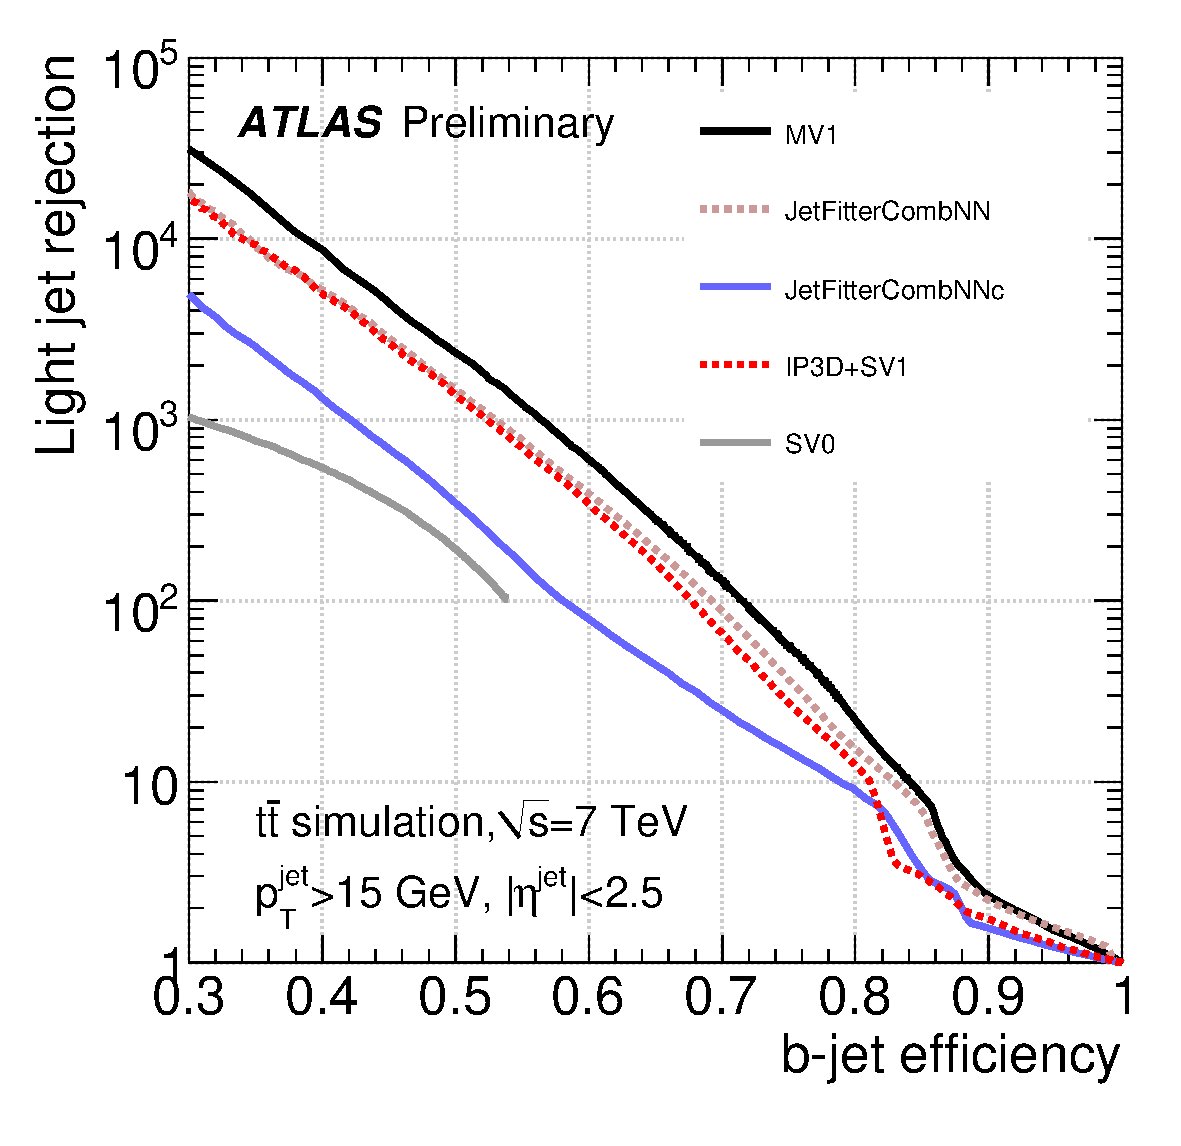
\includegraphics[width=0.45\textwidth]{mj/fig_01a.pdf}}
\subfigure[10q]{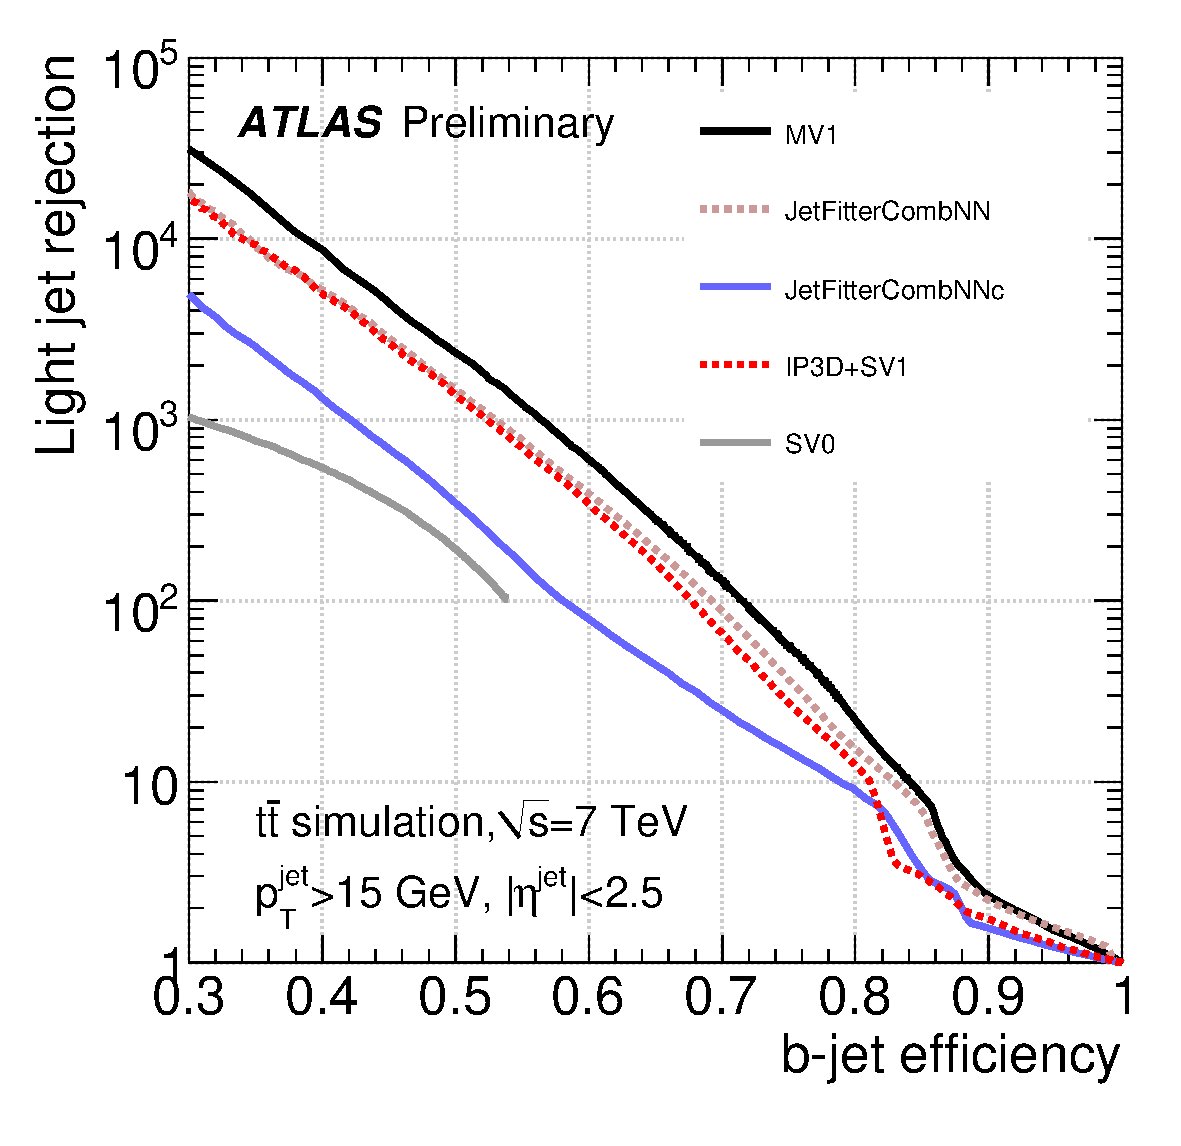
\includegraphics[width=0.45\textwidth]{mj/fig_01a.pdf}}
\label{fig:search:motivation:diagrams}
\caption{Feynman diagrams for a 6q and 10q final state with gluino pair production and RPV decays of the LSP. The 10q final state proceeds through an intermediate neutralino LSP.}
\end{figure}

%%%%%%%%%%%%%%%%%%%%%

Many different possibilities for the flavor structure of the quarks in this diagram exist. As discussed in Section~\ref{chapter:susy:r}, the  $\lambda''_{ijk}$ coupling is actually an anti-symmetric tensor which couples together one up type and two different down type quarks. This means, for example, that the \lsp can decay to a top-bottom-strange triplet, but not a top-bottom-bottom. The most generic assumption is to set all possibilities as equal, as a priori there is no preference for any particular combination. Moreover, there is an additional place for quark flavor to be decided, in the quarks coming from the gluino decay: these are set by the masses of the off-shell squarks in the theory. If the stop was very much lighter than the other squarks, for example, the gluinos would all decay through off-shell stops, leading to only tops from the gluino decays. Again, however, the most generic assumption is to set all squark masses to be degenerate (at 5 TeV, well above threshold), so all decays that are kinematically possible will happen. Ultimately, this means that in decay chains with many hadronically decaying top quarks can have up to 22 quarks in the final state, or as few as 10 in the case where no tops are included in the decays. 

Final states like these have largely been ignored because of the extremely difficult backgrounds: QCD multi-jet processes, which are usually suppressed by \met cuts, are dominant. The problem with QCD is actually two-fold. First, the extremely high cross-section requires very powerful variables to replace the \met cut in order to become sensitive. Additionally, the modeling of QCD backgrounds is also very challenging, generally requiring sophisticated data-driven techniques because of the inadequacy of MC simulation to model the high-multiplicity QCD final states.

An analysis searching for final states of this type is thus very attractive: SUSY could exist at rather low mass, and could be discovered if new analysis strategies and background estimation techniques were developed. Thankfully, jet substructure tools provide an answer to both elements of the problem.

%discuss final state structure, types of quarks, etc?

\section{Why Jet Substructure?}

The best way to understand the utility of jet substruture for this analysis is to consider an event display, as in Figure~\ref{fig:search:motivation:event-displays}. This display shows in the $y/\phi$ plane the \antikt $R=1.0$ Trimmed jets run on a background (left) and signal (right) event. Typically, analyses have used variables such as \Ht-- the sum of the transverse momentum of the jets-- to define a signal region. In this case, the \Ht of the two events is very similar, near $2$~TeV. However, the event on the right shows significantly more \textit{structure} in its jets than the event on the left: QCD jets are generally single-prong, while the jets in the signal have a richer topology.  

%%%%%%%%%%%%%%%%%%%%%

\begin{figure}
\centering
\subfigure[\herwigpp Dijet Background]{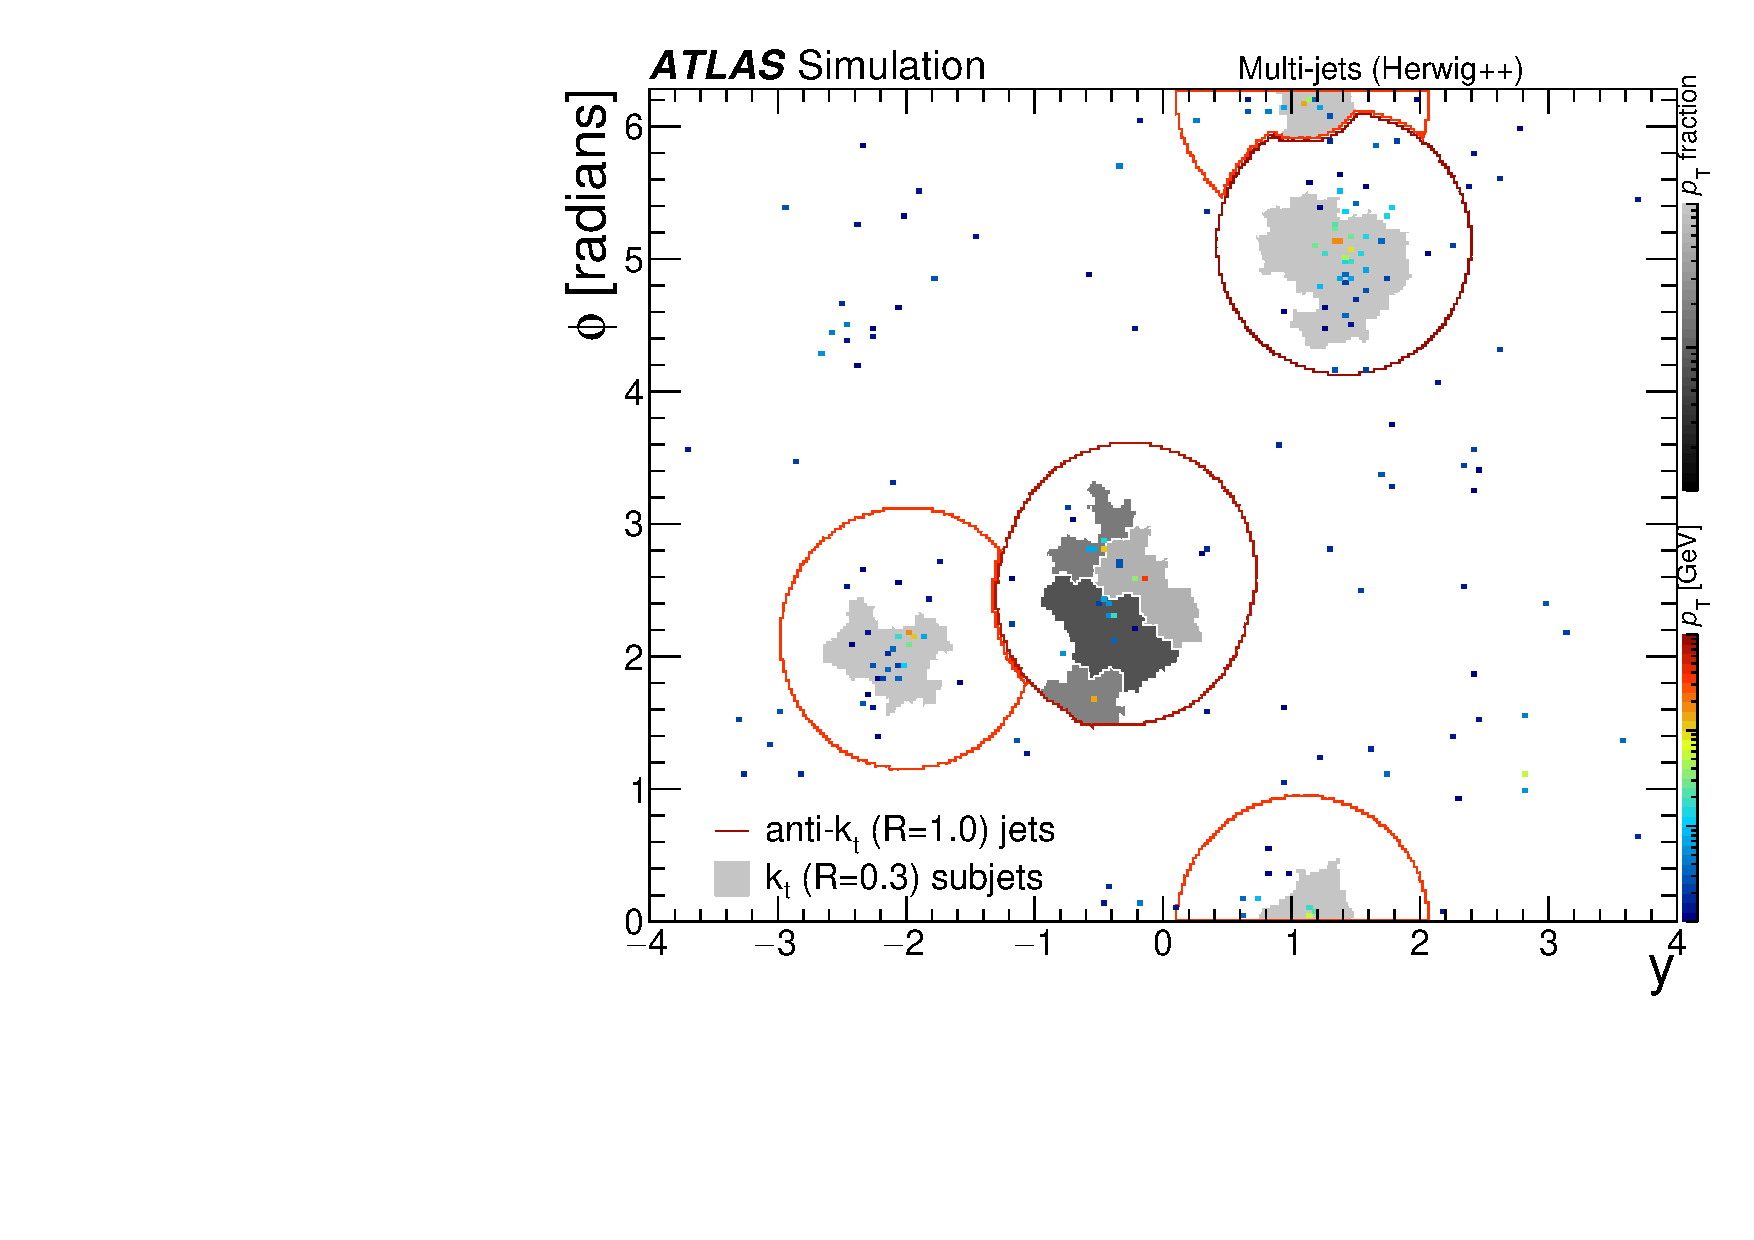
\includegraphics[width=0.45\textwidth]{mj/figaux_08f.pdf}}
\subfigure[\gl-\gl Signal]{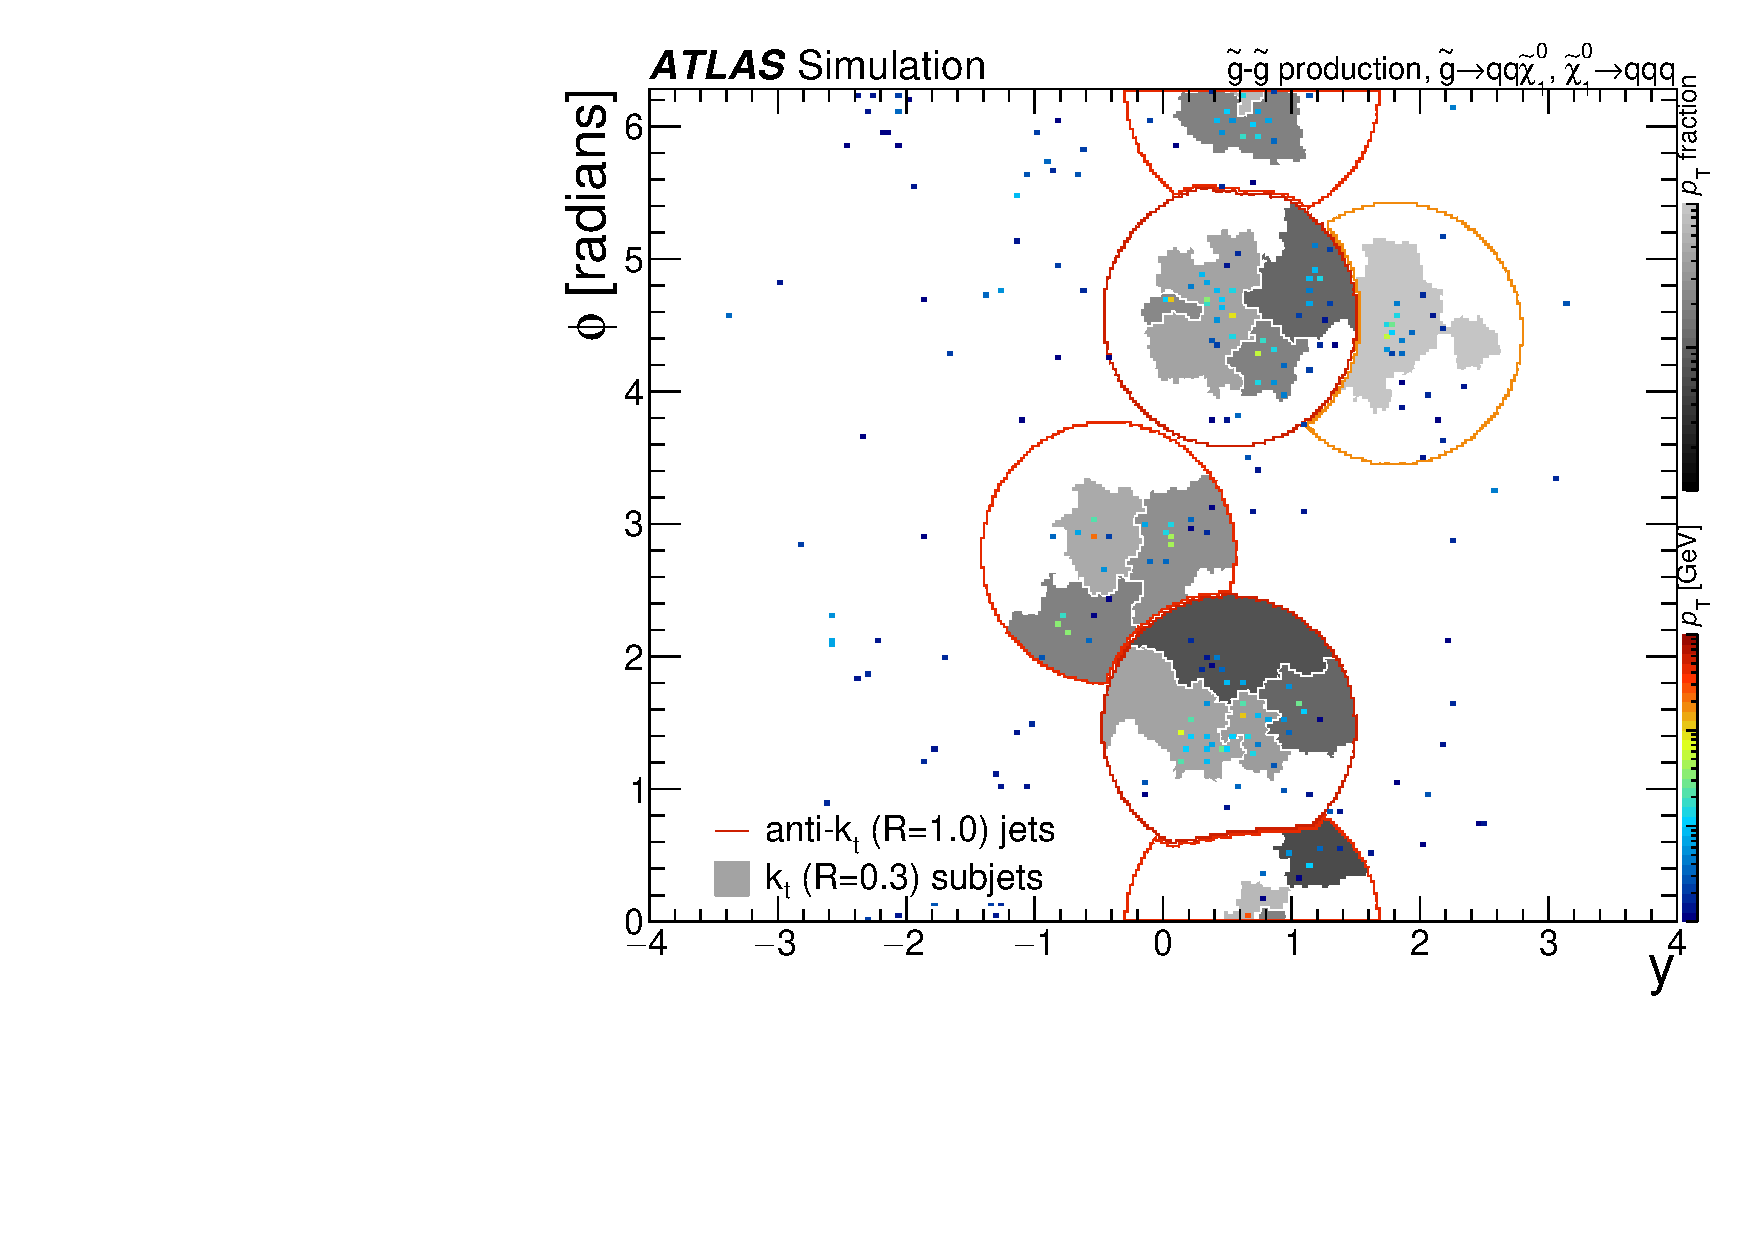
\includegraphics[width=0.45\textwidth]{mj/figaux_06f.pdf}}
\label{fig:search:motivation:event-displays}
\caption{Event displays for background and signal events with very similar \Ht (sum of jet \pt), but very different \textit{jet masses}.}
\end{figure}

%%%%%%%%%%%%%%%%%%%%%

Interestingly, these \largeR jets do not correspond to any particular top quark, or \lsp decay, or \gl decay products: the complicated, high multiplicity environment, along with relatively low \pt for quarks from the \lsp because of 3-body decays, means that most decays are not actually very collimated, and there is a great deal of overlap between quarks. All hope is not lost, however: instead of requiring mass windows, one can simply look for lots of structure. This approach is referred to as \textit{accidental substructure}: the quarks from various parts of the event accidently overlap in the \largeR jets used to reconstruct the event, and simply trying to identify ``lots of structure'' is sufficient to discriminate between signal and background. For this reason, analyses implementing this strategy generally require four \largeR jets in an event, and use the properties of these jets to search for new physics. \editnote{Cite me}

Thus, jet substructure provides a path to discrimination between signal and background, which will be discussed further in Section~\ref{chapter:search:substructure:mj}. Jet substructure actually provides a path for background estimation as well: the \textit{expected structure} of QCD can be measured in control regions and extrapolated to a signal region. This strategy is discussed in Section~\ref{chapter:search:substructure:templates}. \editnote{Cite me}

\subsection{Total Jet Mass, and Other Variables}
	\label{chapter:search:substructure:mj}

A variable like \Ht (or \met) is convenient for analysis because it reduces the complexity of the event to a single scalar variable which quantifies the total energy (or missing energy) in an event. Using this approach as in inspiration, it is also possible to create variables which describe not the amount of energy, but the amount of structure in an event. \editnote{Cite all of me} The simplest possibility is called the \textit{Total Jet Mass}, and is defined as:
%
\begin{equation}
\MJ = \sum_{i=1}^4 M_J^i,
\end{equation}
%
where $i$ iterates over jets with some \pt and $|\eta|$ thresholds (typically 100 GeV and $2.5$ respectively, though the exact \pt cuts on the jets depend on the trigger and signal points, as described in Section~\ref{chapter:search:search}). The $\njet$ requirement is usually set to  This variable is expected to be rather sensitive to the signal: the \largeR jets in a \gl-\gl event are expected to be composed of many quarks each, and thus each have substantial mass compared to dominantly single-prong QCD backgrounds. In Figure~\ref{fig:search:motivation:event-displays}, for example, the background has $\MJ = 260$~GeV, while the signal has $\MJ = 705$~GeV: a substantial difference, even though the \HT is very similar!

There are many other similar variables which can be composed using the structure of the \largeR jets. For example, the \textit{Event-Subjettiness} is defined as:
%
\begin{equation}
T_{MN} = \left(\prod_{i=1}^4 \tau_{MN}\right)^{1/4}.
\end{equation}
%
This is the geometric mean of the n-subjettiness ratios of the leading four jets: the variable is designed to distinguish to search for compatibility of an $M$-prong structure, compared to an $N$-prong, where $M>N$. Typically $M=3$, $N=2$ and $M=2$ and $N=1$ are studied.

Another potentially useful variable is \textit{subjet counting}:
%
\begin{equation}
N_\mathrm{X}^\Sigma = \sum_{i=1}^4 N_\mathrm{X}^J,
\end{equation}
%
i.e. the total number of sub-jets (defined with some algorithm $X$) in the leading four jets in the event~\cite{SubjetCounting}. The number of subjets is again expected to be strongly discriminating: for signal, it should be approximately equal to the number of quarks in the final state, and for background it should be much lower (approximately equal to one subjet per jet). Many different algorithms are possible for defining the subjet algorithm, but two particularly well optimized choices seem most promising~\cite{SubjetCounting}, referred to as the \kt and \ca (though the clustering algorithms are far more involved than the algorithms previously defined). In general, the \kt-counting technique looks for subjets with differing \pt, while the \ca-counting looks for more balanced \pt distributions (following the asymmetry cuts in the original BDRS algorithm~\cite{BDRS}). 

Finally, there are also more kinematic variables which can be constructed from the event (as opposed to the previously discussed structure-based variables). One particularly powerful variable is the difference in pseudo-rapidity between the leading two jets:
%
\begin{equation}
\Delta \eta = |\eta_J^1 - \eta_J^2|.
\end{equation}
%
Supersymmetry is produced in $s$-channel processes, which are generally more centrally produced, and therefore have small $\Delta\eta$, whereas QCD also contains many $t$- and $u$-channel processes which have more forward production, and thefore a very high $\Delta\eta$. It is also possible to define $\Delta y$, the difference in absolute rapidity, but the performance in the two variables is essentially identical.

One last set of variables which can potentially be useful are various ways of using the \pt of the third leading jet, $\pt^3$. Generally multi-jet backgrounds are dominated by di-jet like topologies, where the third jet has relatively low \pt compared to the leading two jets which dominate the event: signal, on the other hand, should have a more even \pt distribution, and therefore a higher $\pt^3$ than background. Likwise, one can look at the ratio $\pt^3/\pt^1$, which normalizes the third \pt by the first. The \pt distributions between signal and background are generally very similar, but in combination with many of the other mass cuts, this can be a useful pre-selection device. 


\subsection{Jet Mass Templates}
	\label{chapter:search:substructure:templates}

The second important aspect of jet substructure in the analysis is in the measurement of the background. Because the main discriminating variables are composed of the \textit{structure} of jets, and the kinematics of these events are less sensitive to new physics, one can form a background prediction based on the structure of jets in a signal-depleted control region, and use the kinematics as a transfer factor into a signal region. These measurements in the control region are formulated as \textit{jet substructure templates}, and are defined in detail in \cite{MassTemplates}. Figure~\ref{fig:search:substructure:template-big-picture} summarizes the procedure: the template, constructed from the training sample, is convoluted with the kinematics of the signal sample, produced a Dressed Sample, which is a distribution of a substructure variable usable for the background estimate.

%%%%%%%%%%%%%%%%

\begin{figure}
\centering
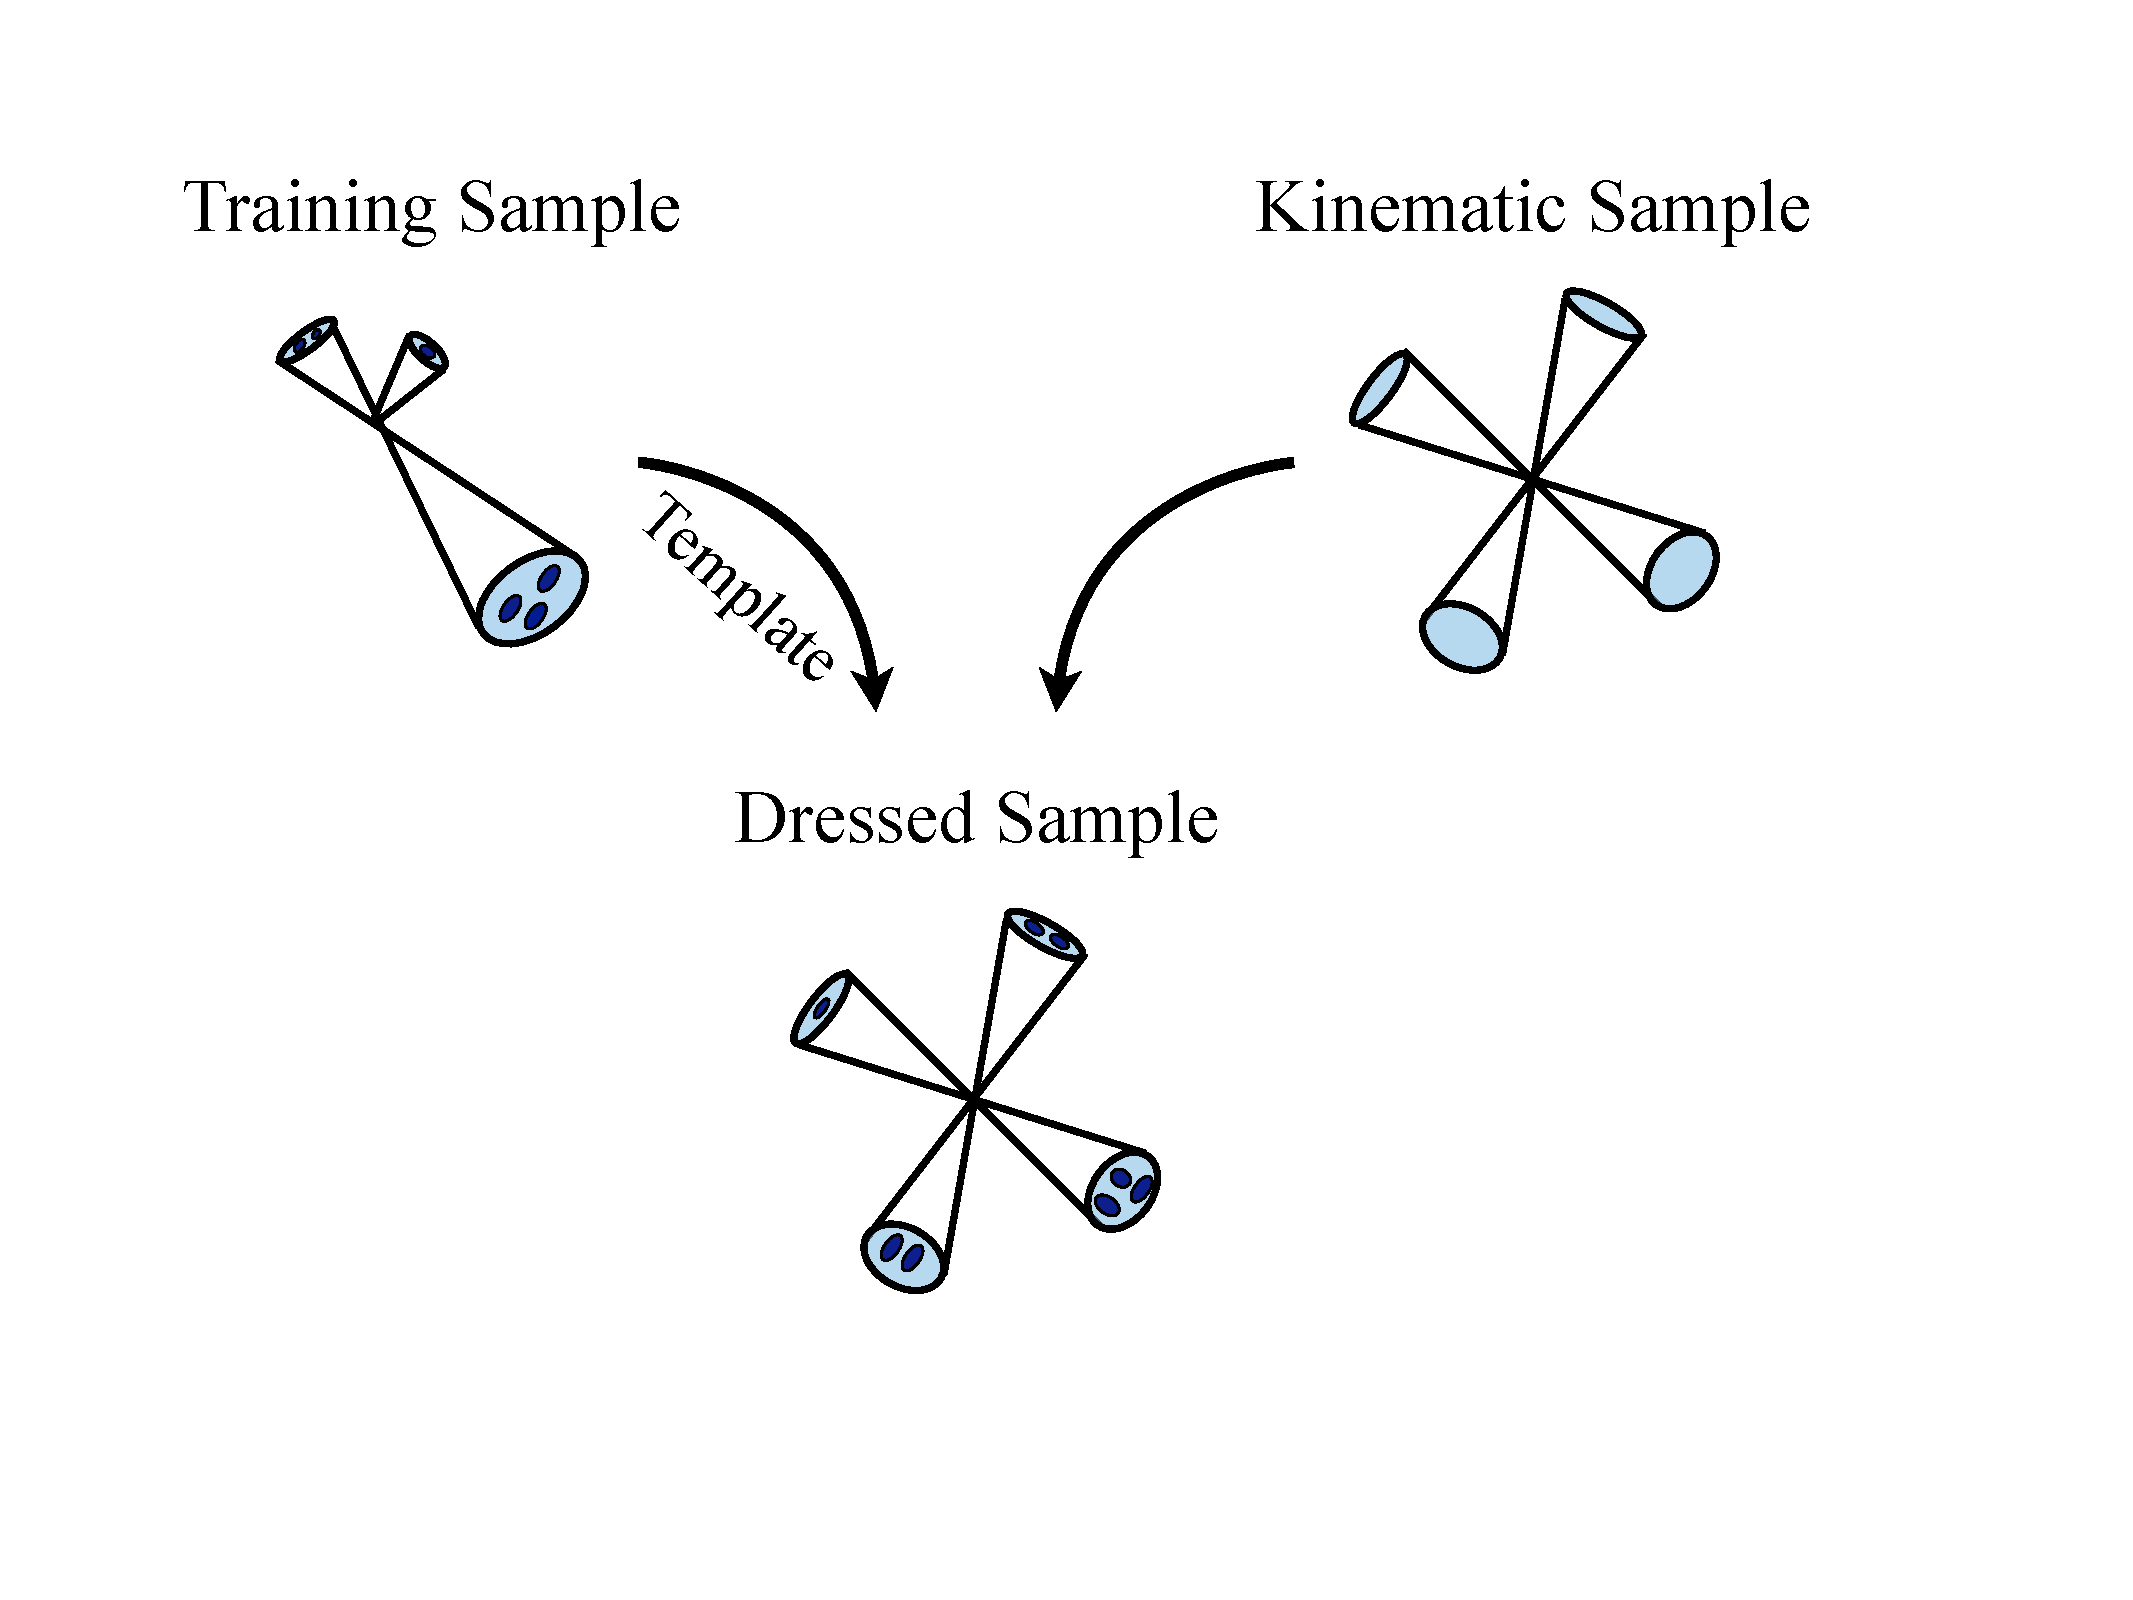
\includegraphics[width=0.7\textwidth]{INT/BigPictureSketch}
\label{fig:search:substructure:template-big-picture}
\caption{The strategy used to develop background estimates using jet substructure templates.}
\end{figure}

%%%%%%%%%%%%%%%%   

The background strategy can be formally described as follows. First, we consider $J_{ij}(z)$, which is a $D$-dimensional vector of variables $z$, which can be ``inputs'' (i.e., kinematic variables like \pt or $\eta$) or ``outputs'' (i.e., substructure variables like mass or $\tau_{21}$), and where $j$ is indexed over events and $i$ for jets in each event. One can define a histogram $T_i = \{J_{i1}, J_{i2}..., J_{iN_T}\}$, which is the multi-dimensional distribution of the variables $z$ defined separately for each jet $i$. To increase statistics, various sums over $i$ can also attempted (for example, using the leading and sub-leading jets together). When $T$ is normalized, it represents a probability distribution function for the jet $i$ to have various properties. However, as this is a highly multi-dimensional object, there can be various regions of this function which are not filled by the training sample, but which are still important for the background estimation. The histograms are therefore smoothed using a Gaussian kernel method, which produces the final templates. In particular, the smoothed template for each jet $i$ is:
%
\begin{equation}
\hat{\rho}_i(z) = \frac{1}{N_T} \sum_{J\in T_i} K_h(z - z_J)
\end{equation}
%
where $K_h$ is the smoothing kernel term, defined as:
%
\begin{equation}
K_h(z) = \frac{1}{(4\pi)^{D/2} \det h} \exp \left[ - \left(h^T h \right)^{-1}_{ij} z^i z^j \right]
\end{equation}
% 
where $h$ is a matrix which describes the width of the kernel. Thus, the template is nothing more than the sum of the multi-dimensional smoothed Gaussians formed by every point in the training. The last point is determining the exact form of the matrix $h$. Usually the best choice is defined by the ``Asymptotic Mean Integrated Squared Error'', which is:
%
\begin{equation}
h_{ij}^\mathrm{amise} = c \hat{\sigma}_{ij} N_T^{-\frac{1}{D+4}}
\end{equation}
%
where $c$ is an $O(1)$ constant, and $\hat{\sigma}$ is the estimate of the square root of the covariance matrix for $\rho(z)$ (the true distribution). For the analysis below, $c=0.01$ is typically used. A schematic diagram summarizing the technique is shown in Figure~\ref{fig:search:substructure:smoothing}

%%%%%%%%%%%%%%%%

\begin{figure}
\centering
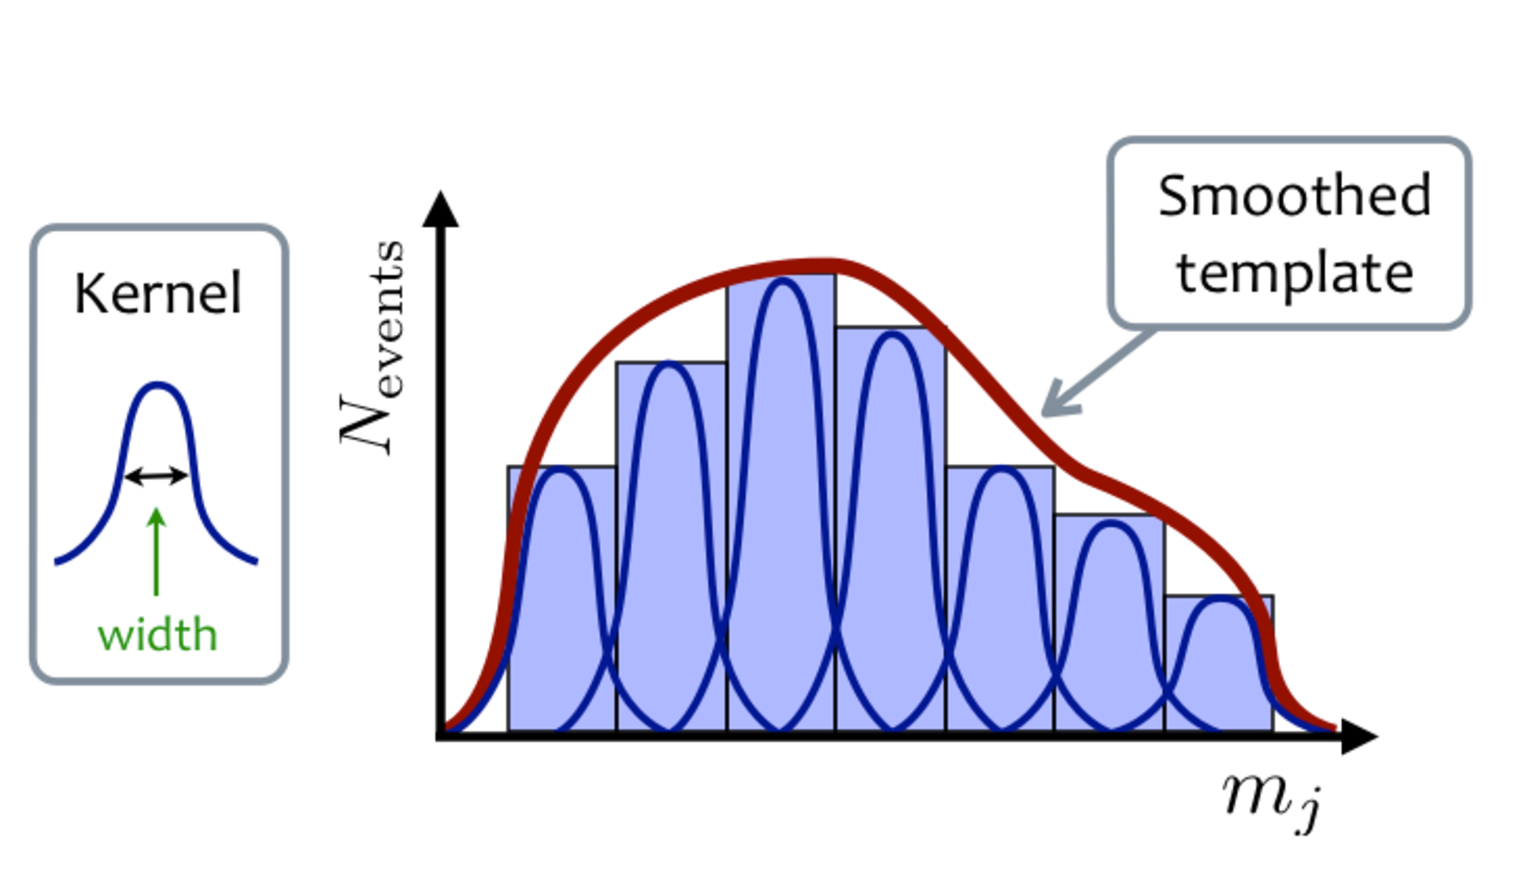
\includegraphics[width=0.7\textwidth]{INT/KernelSmoothing}
\label{fig:search:substructure:smoothing}
\caption{A schematic describing the use of the Gaussian Kernel smoothing method to generate a smoothed template.}
\end{figure}

%%%%%%%%%%%%%%%%  

There are two sources of error due to this smoothing: the \textit{bias} and the \textit{variance}, defined as:
%
\begin{align}
b(z) &= \rho(z) - \hat{\rho}(z)\nonumber\\
v^2(z) &= \langle \hat{\rho(z)}^2 \rangle  - \langle \hat{\rho}(z) \rangle^2.
\end{align}
%
There is also a potential error due to  physics: the extrapolation from a control region to a signal region may not be fully controlled by the kinematic distributions. This is discussed in more detail in Section~\ref{chapter:search:search:background}. 

The bias is an important potential source of error: by definition, it is exactly the difference between the true distribution and the estimate. If we can find an estimate for the bias, we can even correct for this error immediately and derive an improved estimate. In fact, such an estimate can easily be derived by smoothing again the smoothed distribution: this is accurate to first order in $h$ (as shown in detail in Appendix A of \cite{MassTemplates}). The twice smoothed template is:
%
\begin{equation}
\hat{\hat{\rho}}(z) = \int d^D z' \hat{\rho}(z') K_h (z-z')
\end{equation}
% 
and so the bias estimator is:
%
\begin{equation}
\hat{b}(z) = \hat{\hat{\rho}}(z) - \hat{\rho}(z).
\end{equation}
%
This in turn defines the bias corrected template:
%
\begin{equation}
\hat{\rho}^*(z) = \hat{\rho}(z) - \hat{b}(z).
\end{equation}
%
This is the final template (actually, the median of a set of toys of such templates) used for the background estimate. The full difference between the corrected and the un-corrected term (i.e., the full size of $\hat{b}(z)$) is used as a systematic error in the analysis.

Before describing the estimate of the variance $v^2$, we can define how the template $\hat{\rho}^*(z)$ is used to generate a background prediction. In particular, we want to understand the distribution of the substructure variables $x$ as a function of the kinematic variables $k$, which were previously concacted into one vector $z$. Currently, we have a joint probability distribution $\hat{\rho}^*(x,k)$, but we want a \textit{conditional} probability distribution $\hat{\rho}^*{x|k}$. This is derivable as:
%
\begin{equation}
\label{eqn:templates:conditional}
\hat{\rho}^*{x|k} = \frac{\hat{\rho}^*(x,k)}{\hat{\rho}^*(k)} = \frac{\hat{\rho}^*(x,k)}{\int d^d x' \hat{\rho}^*(x',k)} 
\end{equation}
%
where $d$ is the number of kinematic variables in $k$, and $\hat{\rho}^*{x|k}$ defined such that the integral over $x$ is normalized to 1. The remaining question is how to do the non-trivial integral in the denominator of Equation~\ref{eqn:templates:conditional}. One simple solution is to perform the integral using a Monte Carlo approach: each possible value of $x$ (sampled across the full domain of the variable with 500,000 steps, each referred to as $\alpha$) is evaluated simultaneously with the kinematics $k$, returning a weight $w_\alpha$ (or $w^*_\alpha$ for the bias-corrected template) for such a combination. Thus, every kinematic event $k$ creates a distribution for the substructure variables $x$ which is compatible with those kinematics, and this distribution is normalized to 1 (the weight of the particular kinematic event is in total 1). To combine the templates of multiple jets, the product of these weights is computed, as the convolution of the probability density functions of each jet gives the combined probability. For example, for a given event with jet kinematics $k_1$ and $k_2$, one could calculate $M_1 + M_2 = \{w^*_{\alpha,1} w^*_{\alpha,2}\}$, i.e. creating a histogram for the variable $M_1 + M_2$ filled with the product of all the weights; this histogram could then be used to fill another histogram for every event $j$, giving a combined distribution of $M_1 + M_2$ for all the kintematic events in the analysis. This histogram is normalized correctly to the number of events in the dataset: a cut on $M_1 + M_2$, either creating mass windows or a simple cut-and-count region, can be compared directly to the observed mass distribution to search for new physics.

There is on subtlety to this point: if new physics is present, then the ``extra'' events from new physics would be included in the normalization-- and so would pass undetected in the inclusive distribution. However, since the \pt of new physics and QCD is the same, the bulk of the `predicted' masses would fall in the low mass range, near the peak of QCD-- the tails would see a very small, sub-percent, additional contribution (as they are a factor of a million or lower compared to the peak in QCD). Thus, the standard interpretation of a background prediction, with a signal appearing as an additive excess, is reasonable in the tails of the mass distribution, even though the overall normalization would be preserved (and so in the case of an observation of new physics, the peak would see a slight under-prediction of the mass). The technique in \cite{MassTemplates} avoided this issue by using normal MC simulation, normalized to luminosity, to create the kinematic sample used to create the background prediction: however, as multi-jet \pt spectra are notoriously difficult to normalize, and using an MC simulation would add JES related systematics, the data-only technique is used by this analysis.

Finally, the direct analytical calculation of the variance is very difficult, but a different straightforward technique is easy to apply. \textit{Bootstrapping}-- i.e., generating toys via varying the number of events in each bin in the histogram $T_i$ via the Poisson distribution cenetered at the bin value, performing the same procedure on all the toys, and calculating a new final histogram for each toy. Then, each mass bin of interest can assessed by the full ensemble of these toy histograms: the median is used as the nominal value, and the $\pm 1\sigma$ values (i.e., the 68th and 32nd sorted entries when using 100 toys) are used to bracket the derived variance. This corresponds to the statistical uncertainty of the templates. Note that because the variance computed in this way is exact (up to fluctuations based on the number of toys) while the bias is a first order approximation, typically $c$, the constant in the rule-of-thumb, is selected to \textit{undersmooth}: this raises the size of the variance (which we know very well) but lowers the size of the bias. In the limit that the variance dominates, higher order corrections to the bias estimation do not matter.

Thus, by measuring jet properties (such as the mass, or the n-subjettiness) as a function of the kinematic variables using mass templates, one can use jet substructure as a background estimation technique. In this sense, jets are used as a tool to divide up the event, and characterize the expected properities of portions of the detector.
%

\section{Constructing a Search}
\label{chapter:search:search}

With the general principles of a substructure based RPV SUSY search defined, the following subsections define the analysis of \cite{RPVSUSY}, which was the first search for the 10-quark model previously described.


\subsection{Optimization}
\label{chapter:search:search:optimization}

While the complicated multi-jet backgrounds generally require the previously discussed data-driven background techniques to create reliable predictions for the final analysis, it is cumbersome to use these techniques for performing the optimization over a large number of possible variables. For this reason, we use signal MC and \herwigpp di-jet MC to explore the previously defined variables, and to select the most useful way of defining the analysis. The goal is to find two variables which are \textit{uncorrelated}: that is, that they provide discrimination power more or less independently of each other. In this way, one variable can be used to define signal and control regions, while another can be used as the final cut in the signal region to define the precise search region.

One initial question is the number of jets required in the signal region, and which jet algorithm to use. The jet algorithm is the \antikt $R=1.0$, built from locally calibrated topological clusters, with trimming of $\Rsub = 0.3$ and $\fcut > 5\%$, as described in Chapter~\ref{chapter:jet-reconstruction}. These jets are available to 100 GeV: below this point, the calibrations and uncertainties are not valid. An initial optimization found that requiring $\geq 4$ jets above this threshold was the most effective strategy: exactly 3-jet and lower multiplicities are background dominated, while the signal efficiency for a $> 5$ is rather low. Note that the requirement on 4 jets is inclusive: jets with higher multiplicity are allowed. It should also be noted that jets are required to fall with $|\eta| < 2.5$, the region of validity of the systematic uncertainty measurement: jets outside of this requirement are not considered, so the ordering of the 4 jets in the analysis takes into account only jets within this proper fiducial region.

\subsubsection{1D Optimization}

Figures~\ref{fig:search:search:optimization:HT}, \ref{fig:search:search:optimization:MJ}, \ref{fig:search:search:optimization:T21}, \ref{fig:search:search:optimization:T32}, \ref{fig:search:search:optimization:NCA}, \ref{fig:search:search:optimization:NKT}, \ref{fig:search:search:optimization:PT31}, and \ref{fig:search:search:optimization:DEta} show the distribution of a given variable for both signal (in colors) and background (in black) on the left, while the right shows the signal efficiency vs. background rejection (defined as 1/(background efficiency)). Several trends are clear for most of the variables: higher \mgluino raises the energy of the event and increases the discrimination power of most of the variables. Some variables have less dependence on this, however, such as $T_{21}$ and $T_{32}$.

%%%%%%%%%%%%%%%%%%%%%

\begin{figure}
\centering
\subfigure{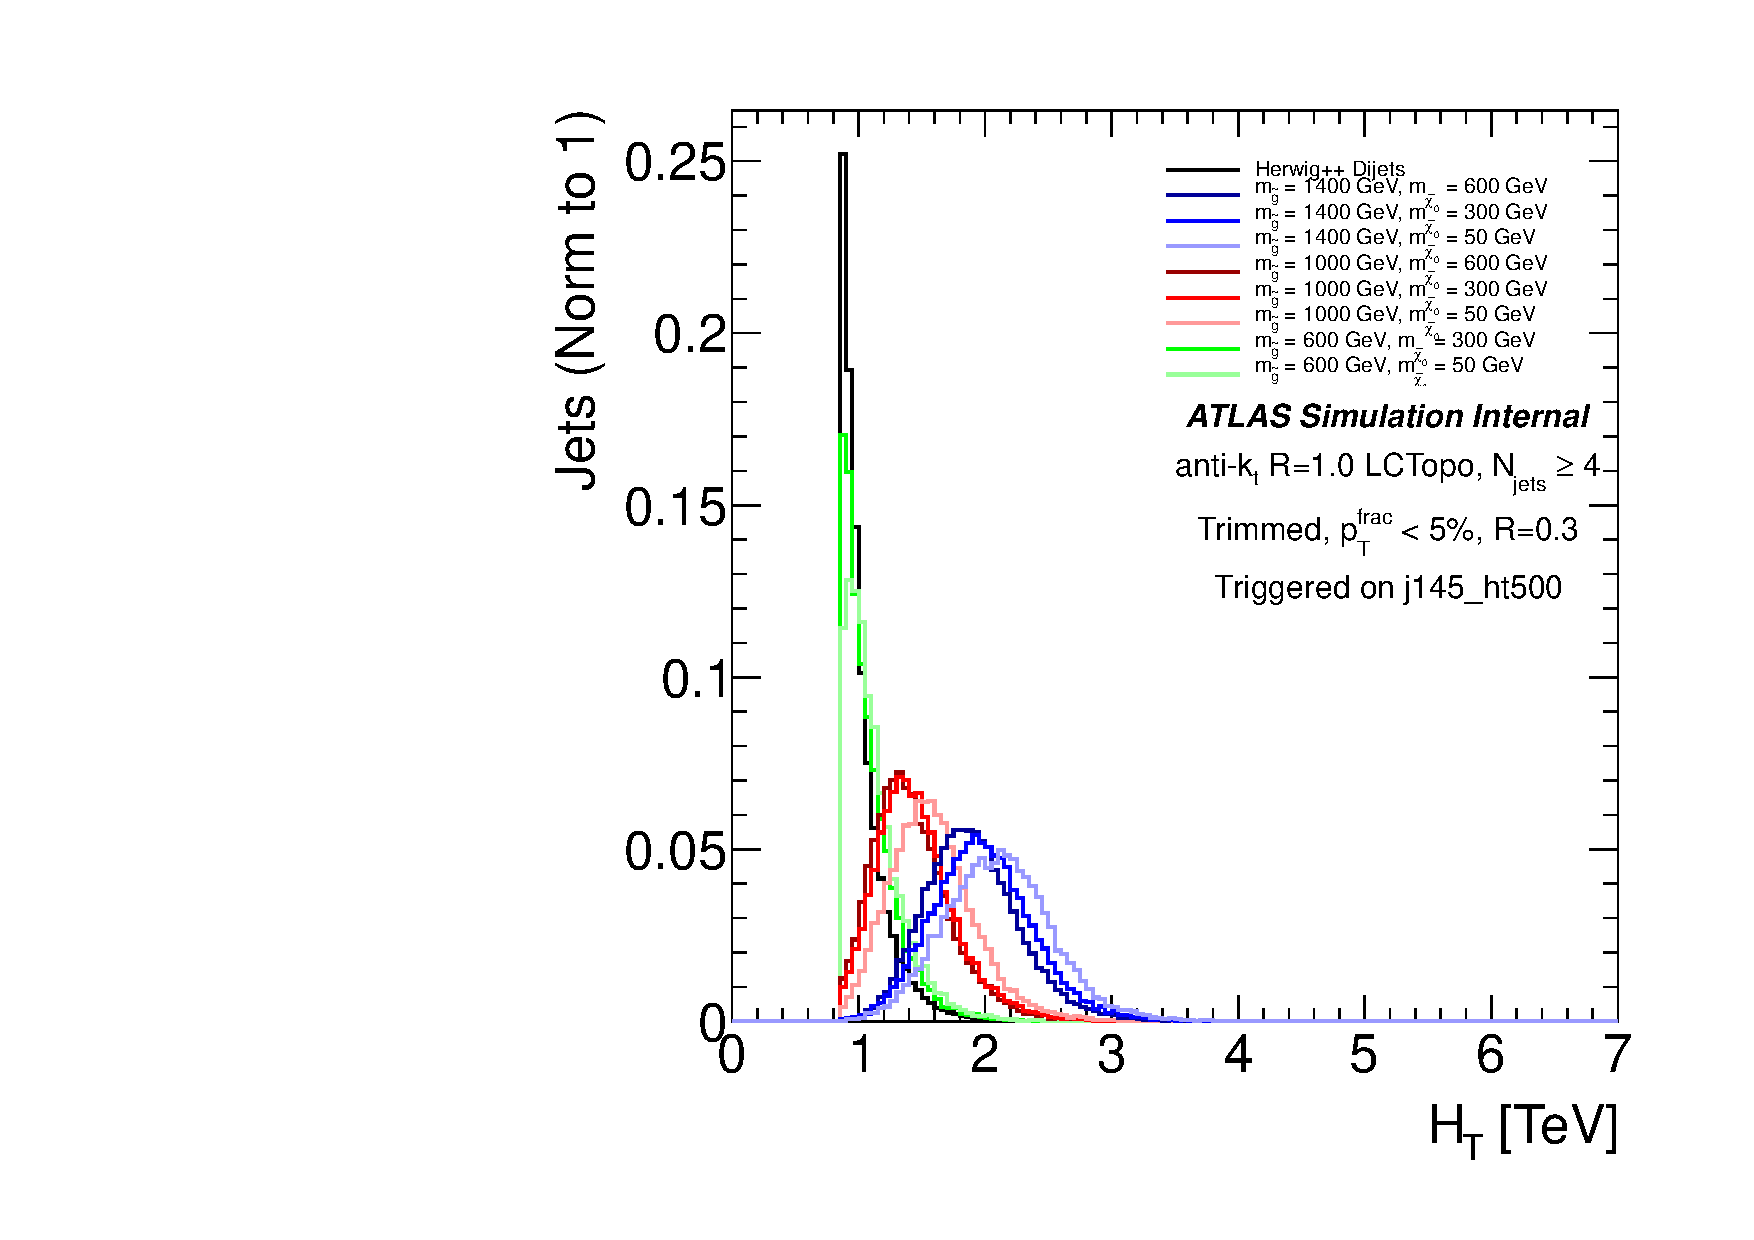
\includegraphics[width=0.45\textwidth]{INT/AntiKt10LCTopoTrimmedPtFrac5SmallR30_j145_ht500_NjetIncl_NFatJetMin4_HT4_RPVGluino.pdf}}
\subfigure{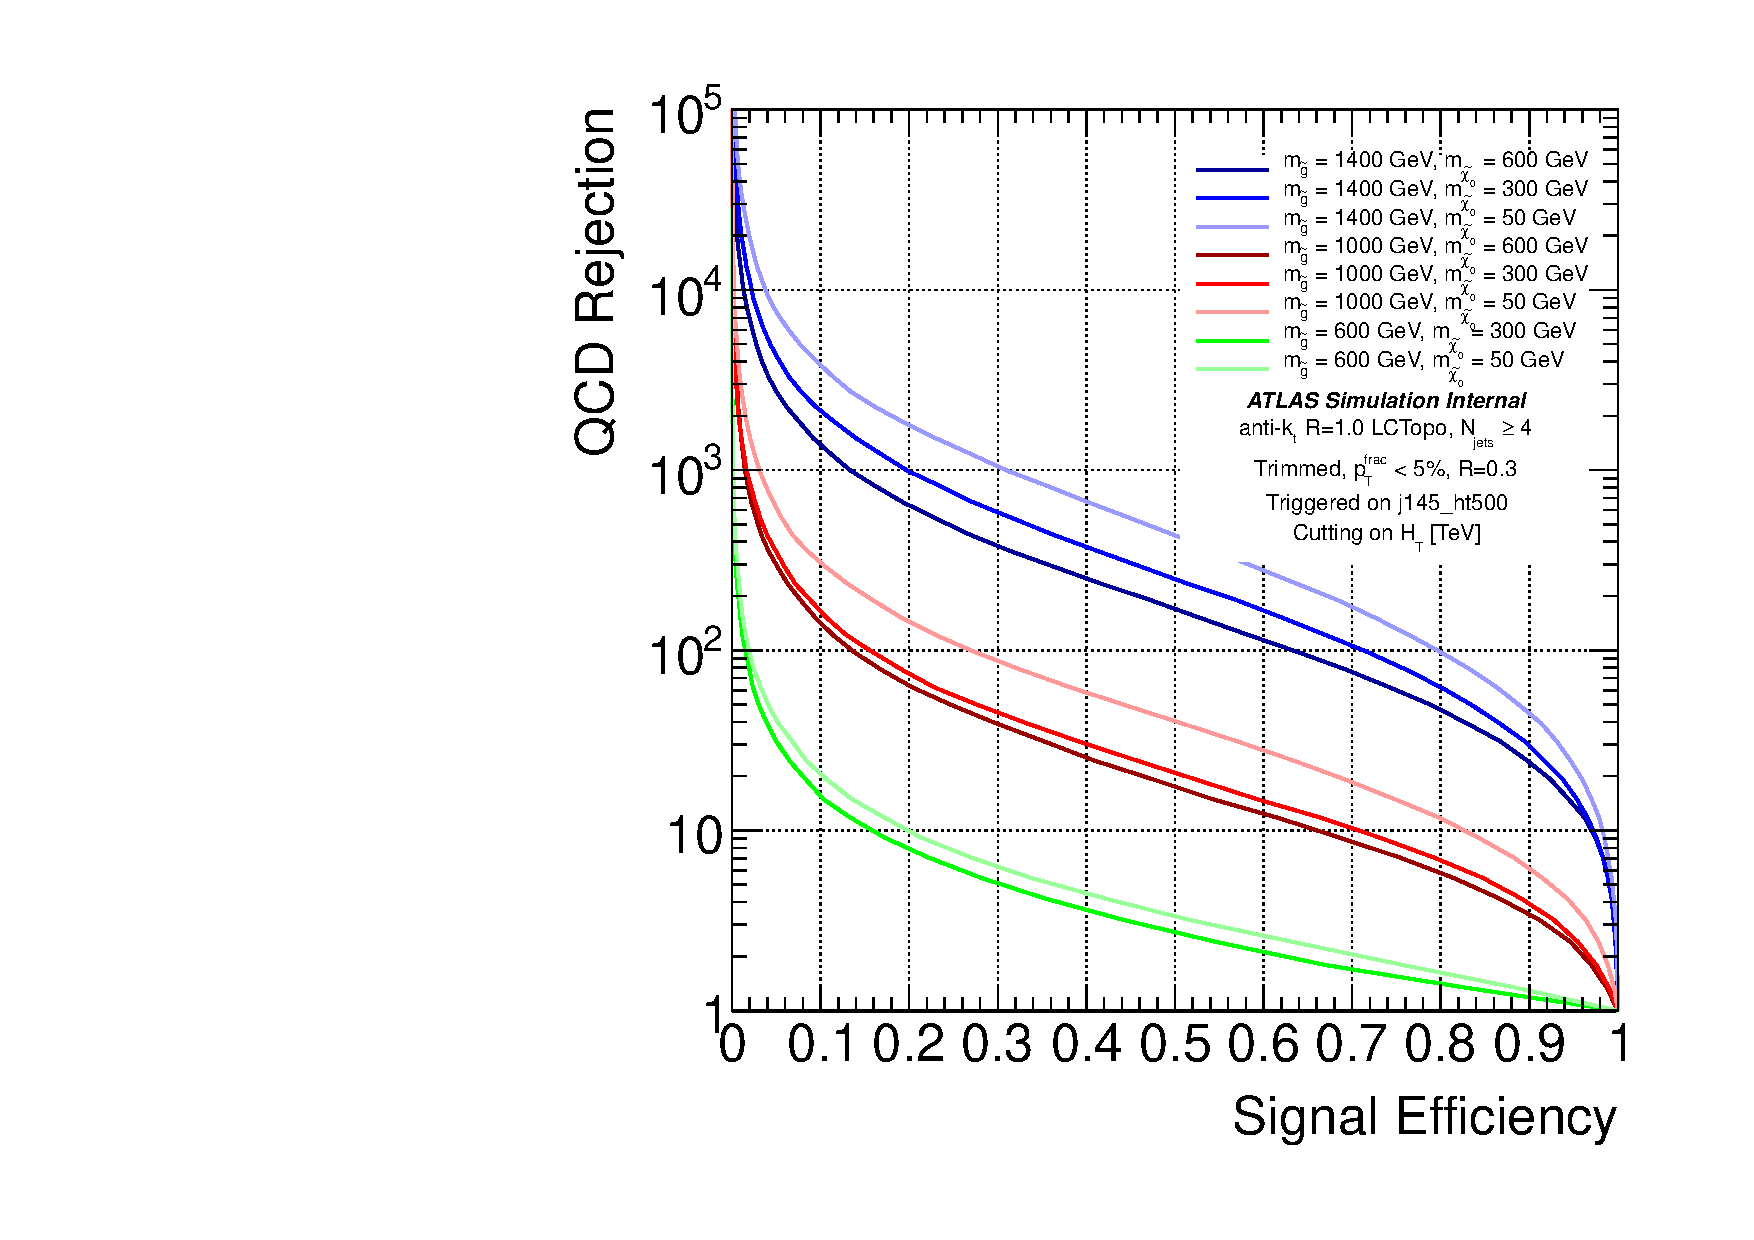
\includegraphics[width=0.45\textwidth]{INT/AntiKt10LCTopoTrimmedPtFrac5SmallR30_j145_ht500_NjetIncl_NFatJetMin4_HT4_g_RPVGluino}}
\label{fig:search:search:optimization:HT}
\caption{Distribution of $H_T = \sum_{i=1}^4 \pT^J$, a typical variable used to measure the energy in an event and discriminate between signal and background. Several signal mass points and the \herwigpp di-jet background are shown. The right-hand plot shows the signal efficiency vs. background rejection of a scan of possible cuts on the \HT distribution.}
\end{figure}

%%%%%%%%%%%%%%%%%%%%%


%%%%%%%%%%%%%%%%%%%%%

\begin{figure}
\centering
\subfigure{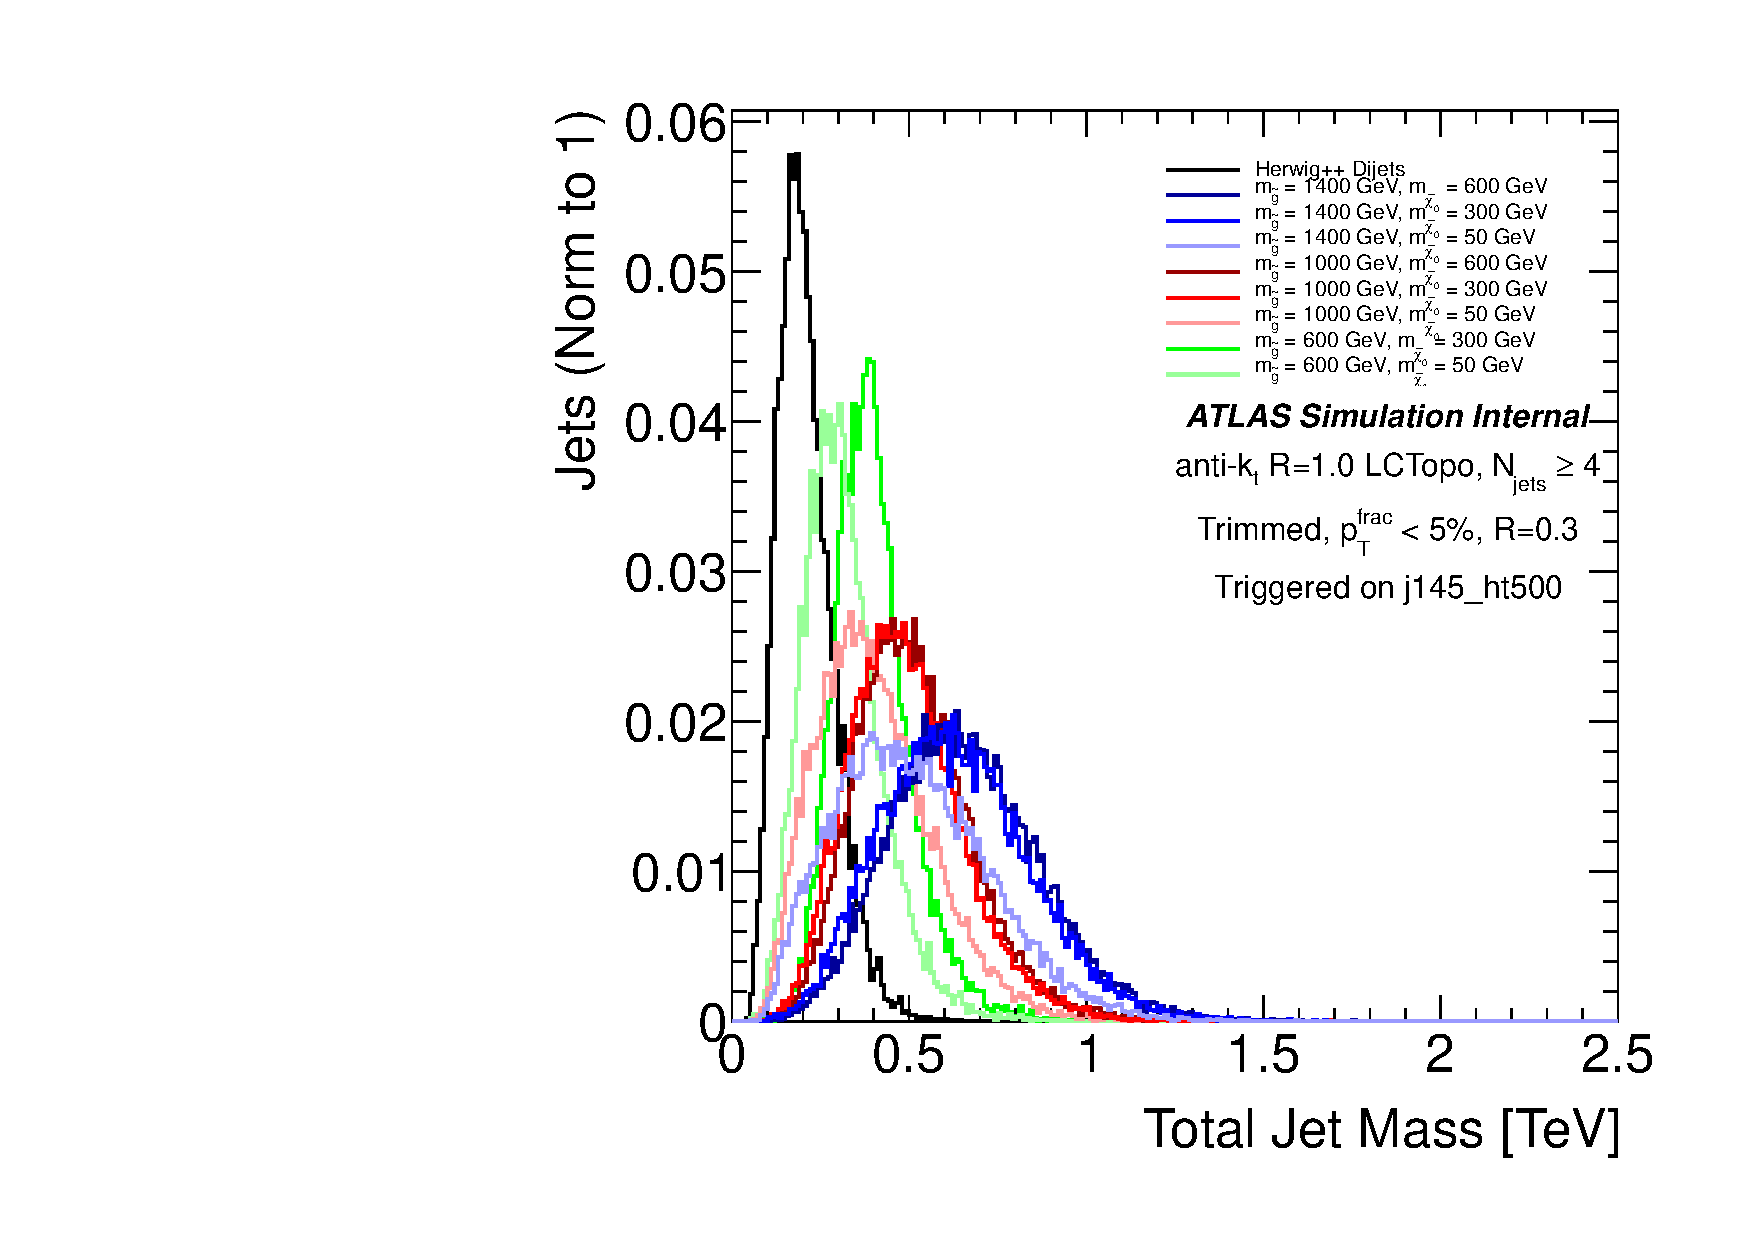
\includegraphics[width=0.45\textwidth]{INT/AntiKt10LCTopoTrimmedPtFrac5SmallR30_j145_ht500_NjetIncl_NFatJetMin4_MJ4_RPVGluino.pdf}}
\subfigure{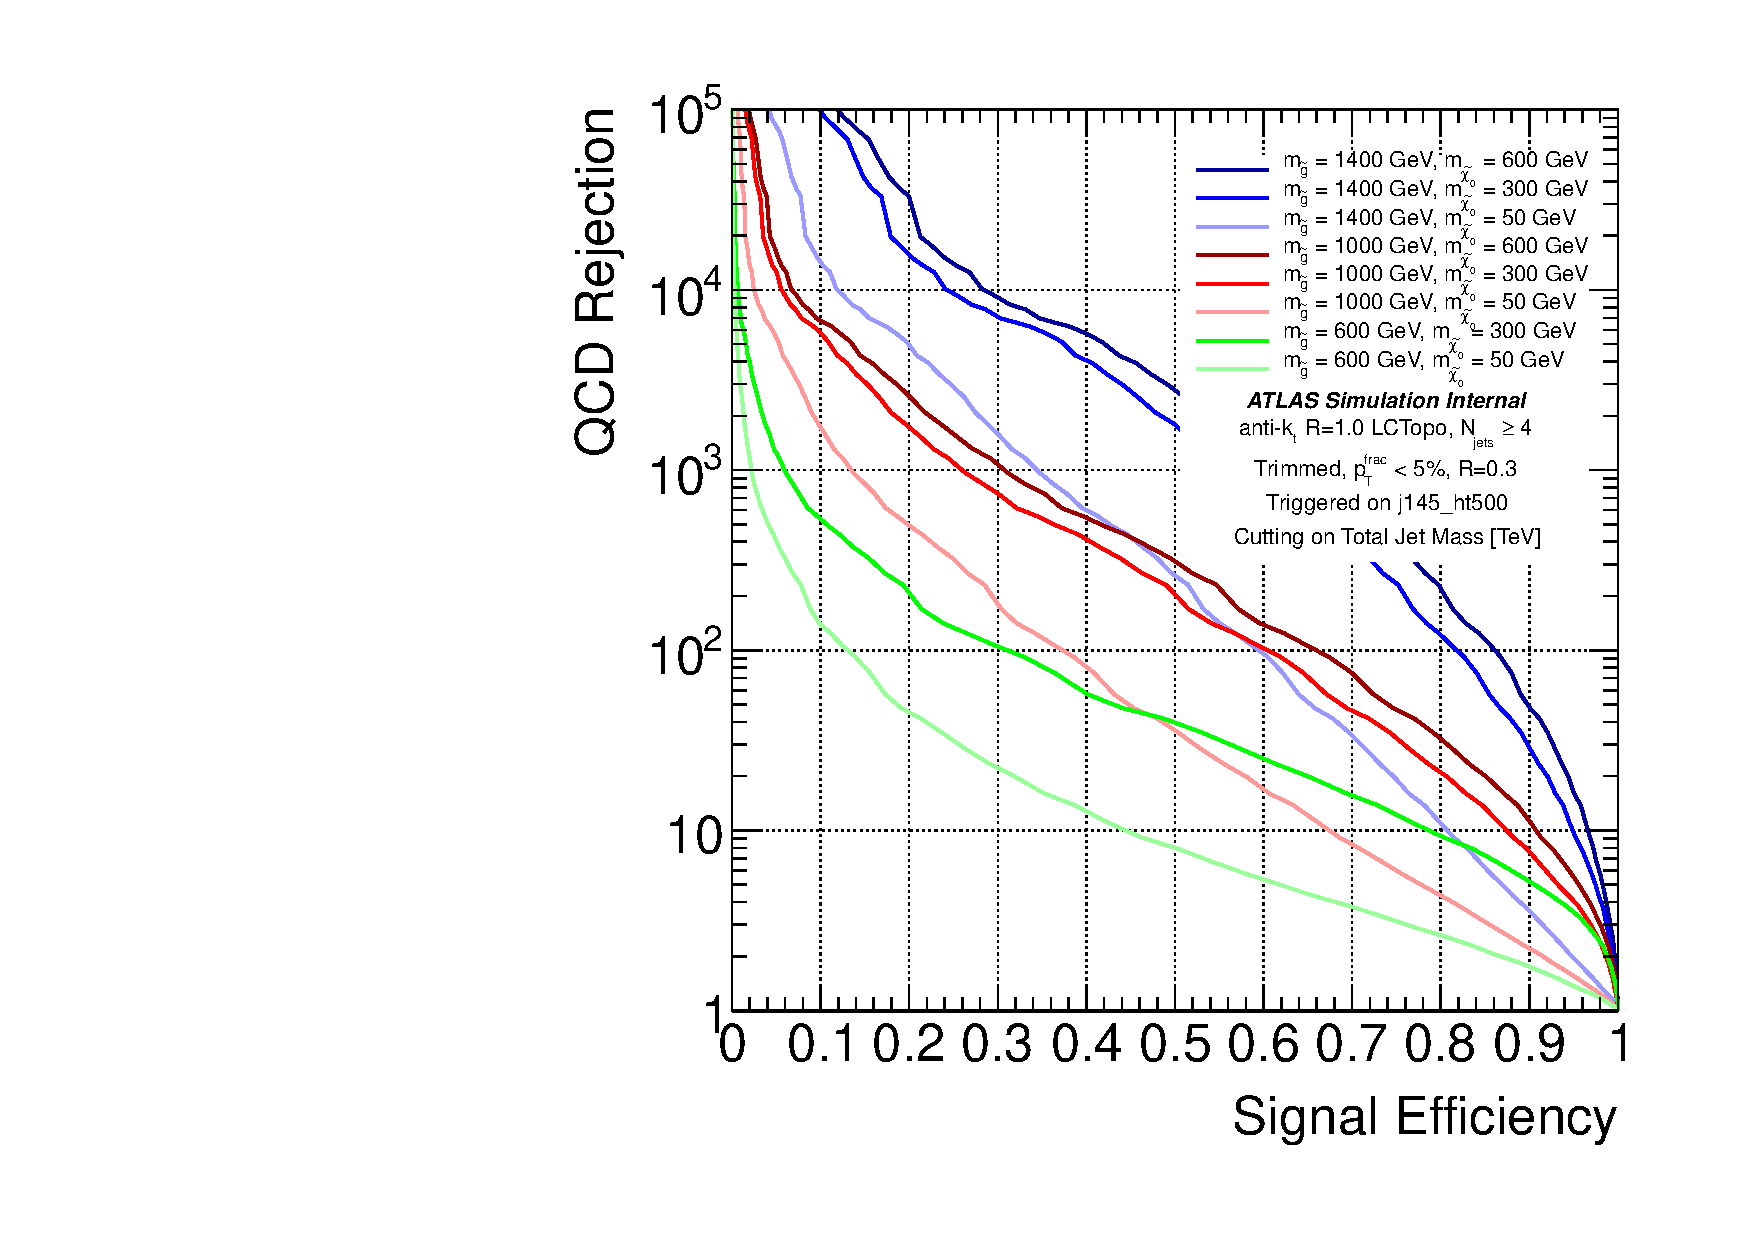
\includegraphics[width=0.45\textwidth]{INT/AntiKt10LCTopoTrimmedPtFrac5SmallR30_j145_ht500_NjetIncl_NFatJetMin4_MJ4_g_RPVGluino}}
\label{fig:search:search:optimization:MJ}
\caption{Distribution of \MJ, a variable describing the total mass in the event. Several signal mass points and the \herwigpp di-jet background are shown. The right-hand plot shows the signal efficiency vs. background rejection of a scan of possible cuts on the \MJ distribution.}
\end{figure}

%%%%%%%%%%%%%%%%%%%%%


%%%%%%%%%%%%%%%%%%%%%

\begin{figure}
\centering
\subfigure{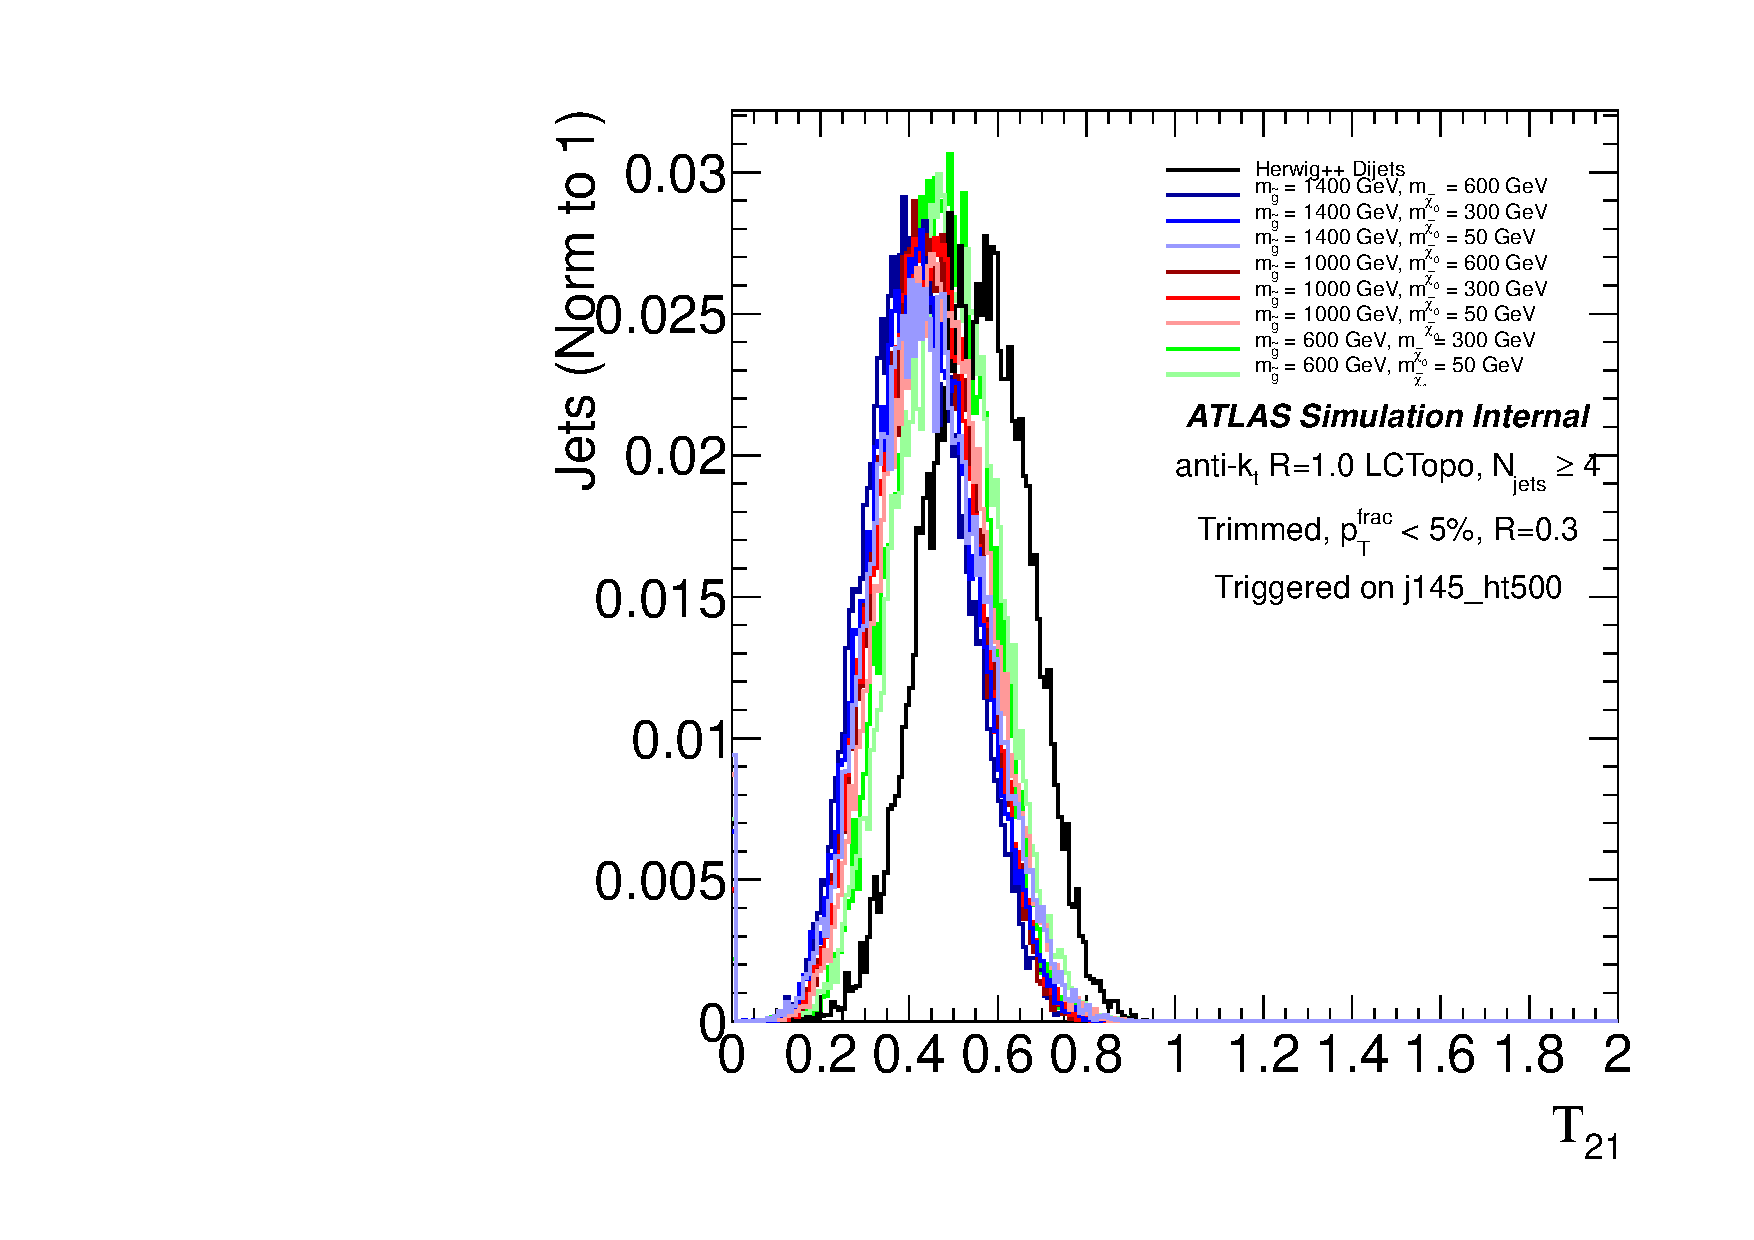
\includegraphics[width=0.45\textwidth]{INT/AntiKt10LCTopoTrimmedPtFrac5SmallR30_j145_ht500_NjetIncl_NFatJetMin4_4T21_RPVGluino.pdf}}
\subfigure{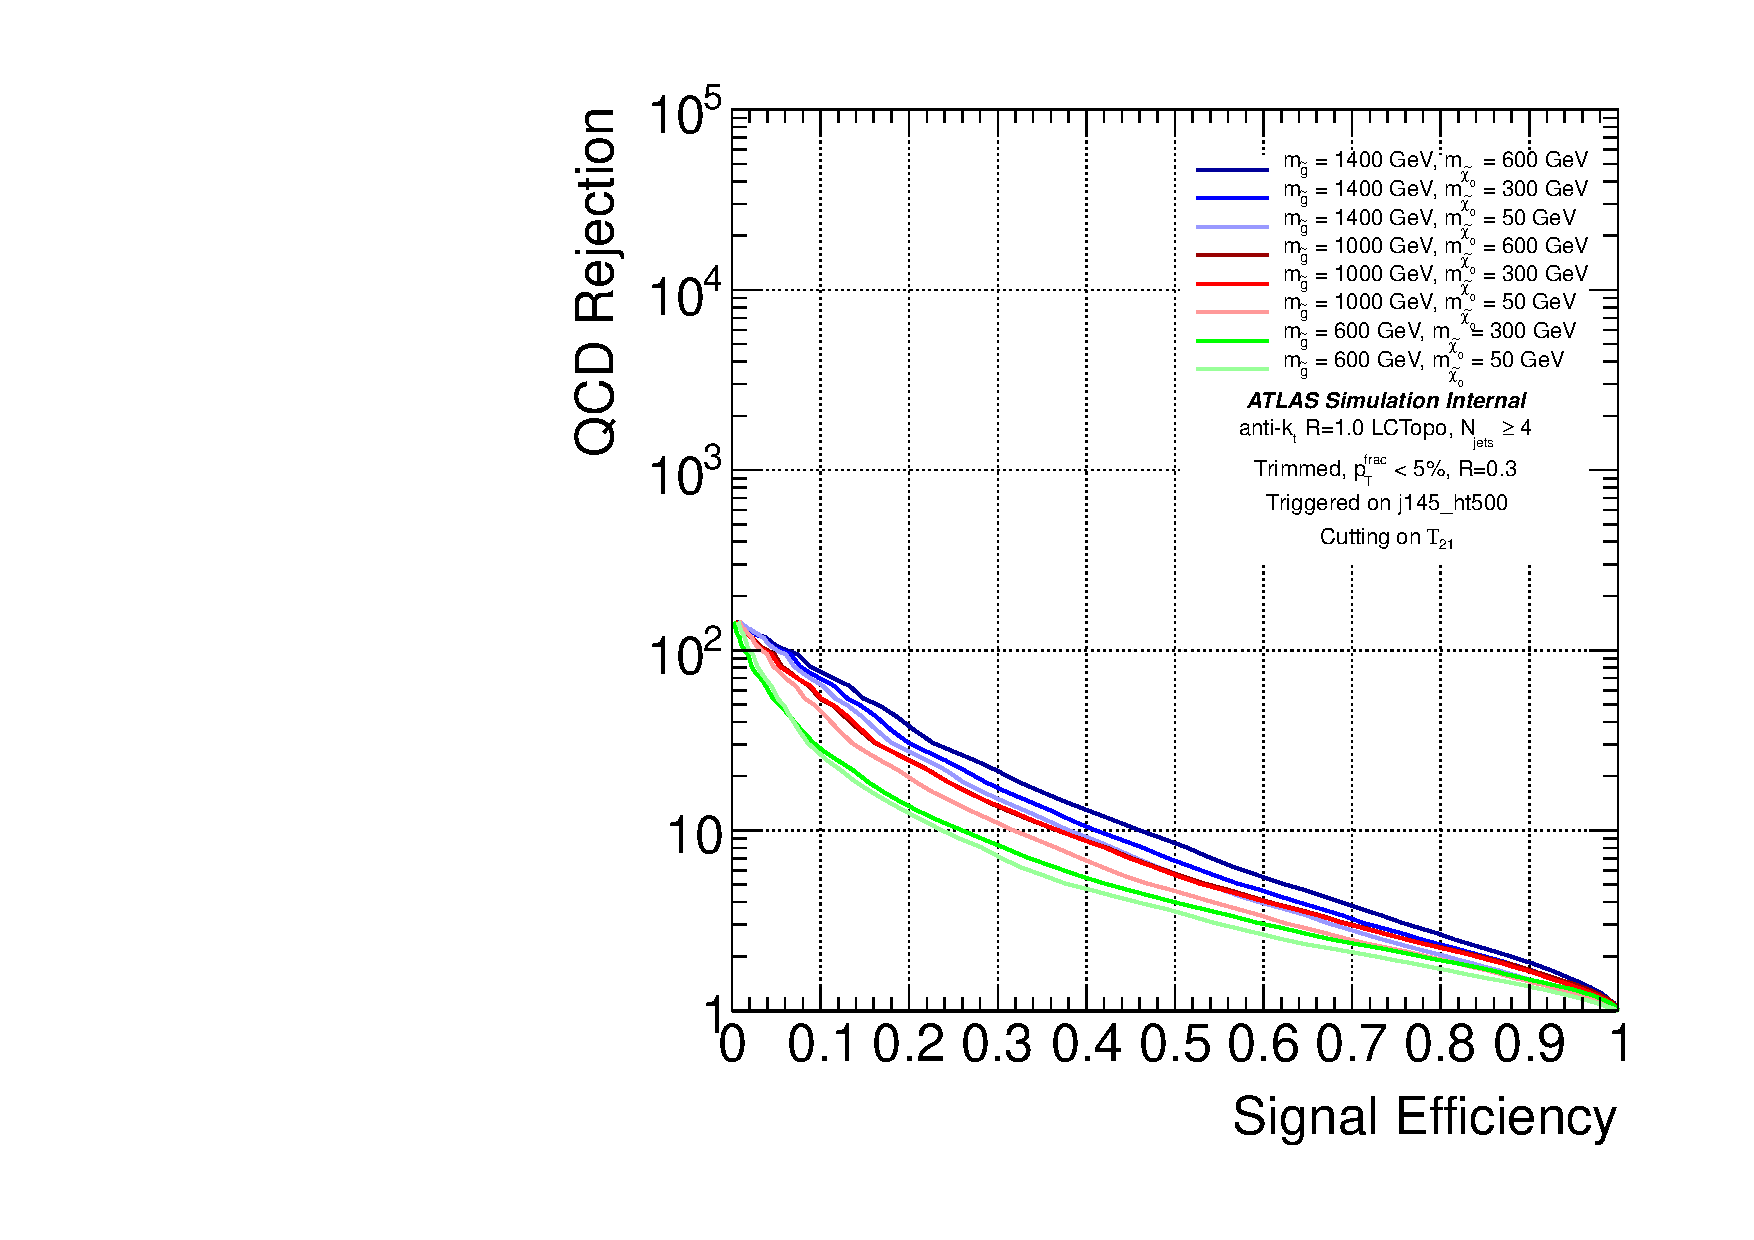
\includegraphics[width=0.45\textwidth]{INT/AntiKt10LCTopoTrimmedPtFrac5SmallR30_j145_ht500_NjetIncl_NFatJetMin4_4T21_g_RPVGluino}}
\label{fig:search:search:optimization:T21}
\caption{Distribution of $T_{21}$, a variable describing the average n-subjettiness ($\tau_{21}$) in the event. Several signal mass points and the \herwigpp di-jet background are shown. The right-hand plot shows the signal efficiency vs. background rejection of a scan of possible cuts on the $T_{21}$ distribution.}
\end{figure}

%%%%%%%%%%%%%%%%%%%%%

%%%%%%%%%%%%%%%%%%%%%

\begin{figure}
\centering
\subfigure{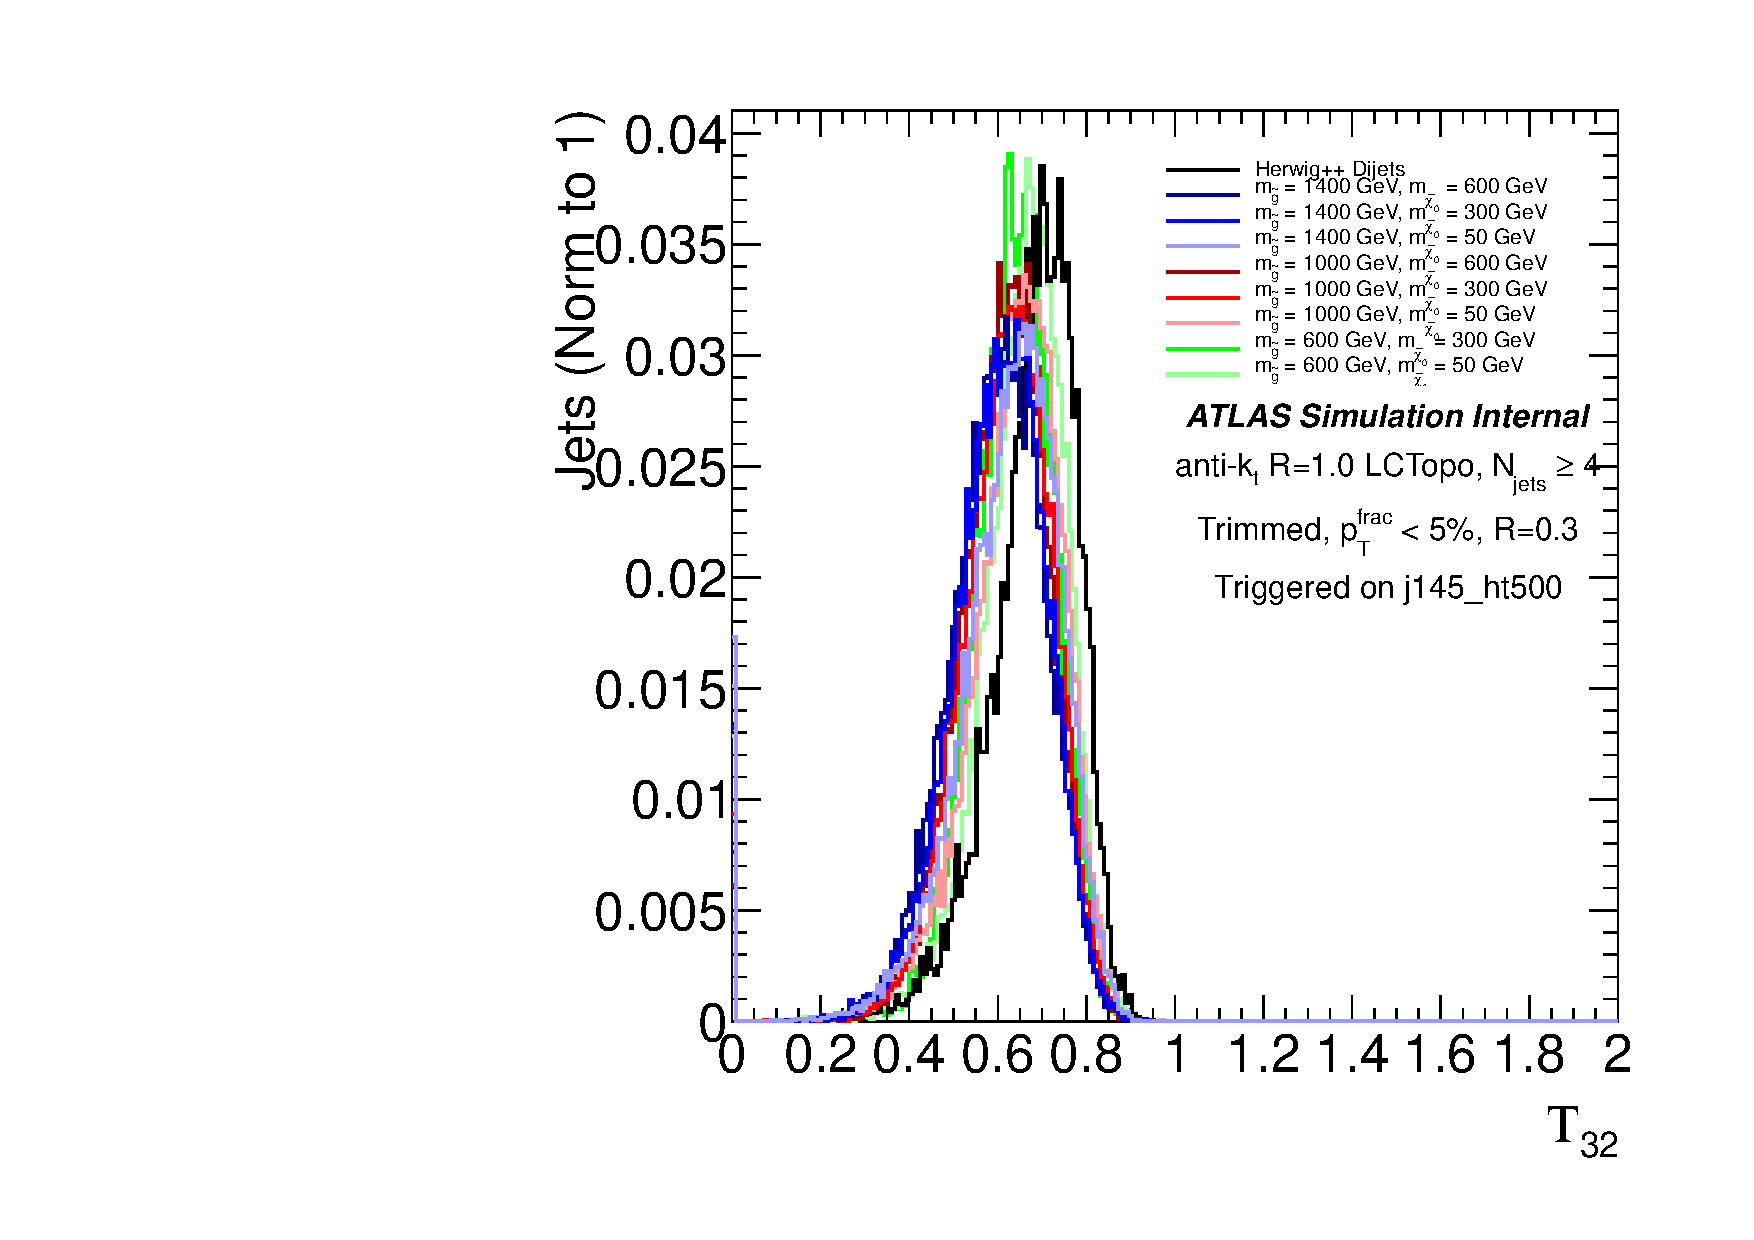
\includegraphics[width=0.45\textwidth]{INT/AntiKt10LCTopoTrimmedPtFrac5SmallR30_j145_ht500_NjetIncl_NFatJetMin4_4T32_RPVGluino.pdf}}
\subfigure{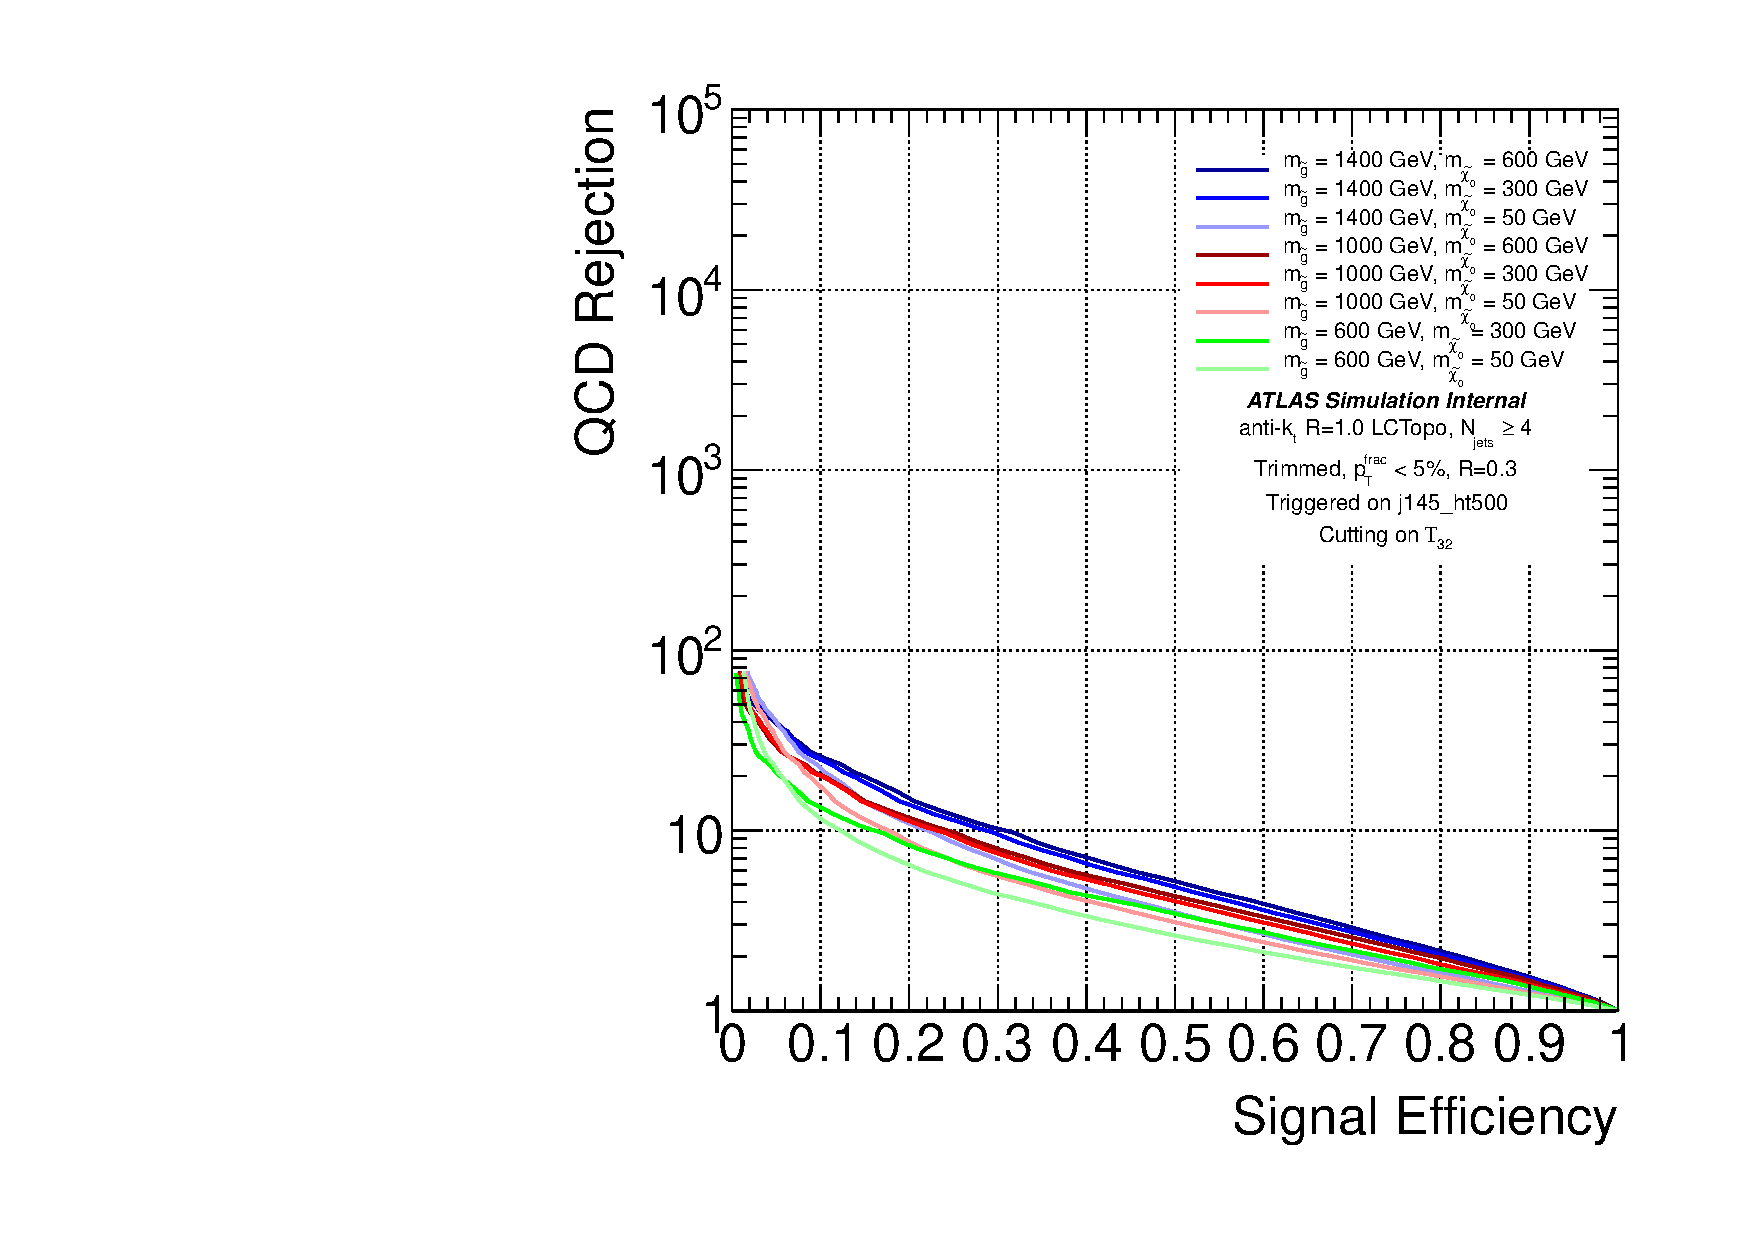
\includegraphics[width=0.45\textwidth]{INT/AntiKt10LCTopoTrimmedPtFrac5SmallR30_j145_ht500_NjetIncl_NFatJetMin4_4T32_g_RPVGluino}}
\label{fig:search:search:optimization:T32}
\caption{Distribution of $T_{32}$, a variable describing the average n-subjettiness ($\tau_{32}$) in the event. Several signal mass points and the \herwigpp di-jet background are shown. The right-hand plot shows the signal efficiency vs. background rejection of a scan of possible cuts on the $T_{32}$ distribution.}
\end{figure}

%%%%%%%%%%%%%%%%%%%%%



%%%%%%%%%%%%%%%%%%%%%

\begin{figure}
\centering
\subfigure{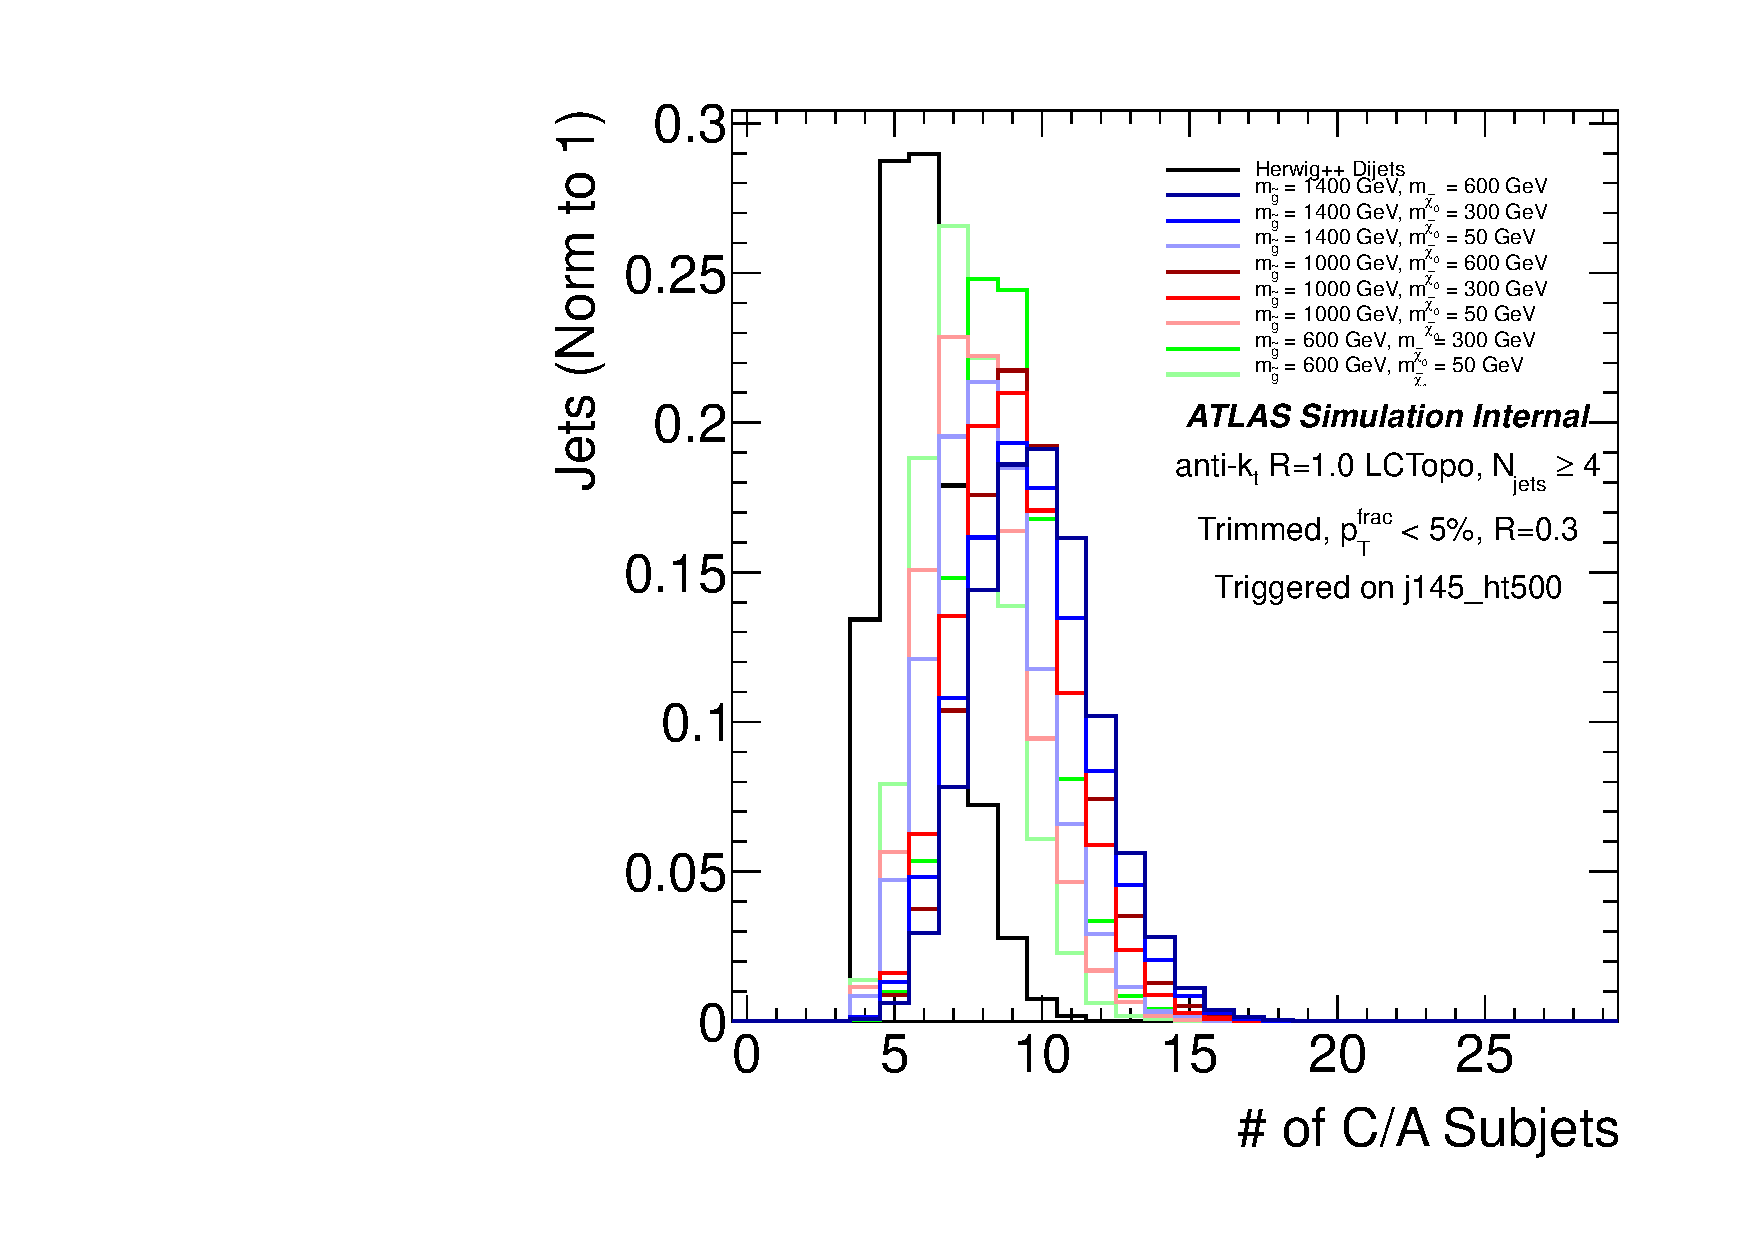
\includegraphics[width=0.45\textwidth]{INT/AntiKt10LCTopoTrimmedPtFrac5SmallR30_j145_ht500_NjetIncl_NFatJetMin4_NCASub4_RPVGluino.pdf}}
\subfigure{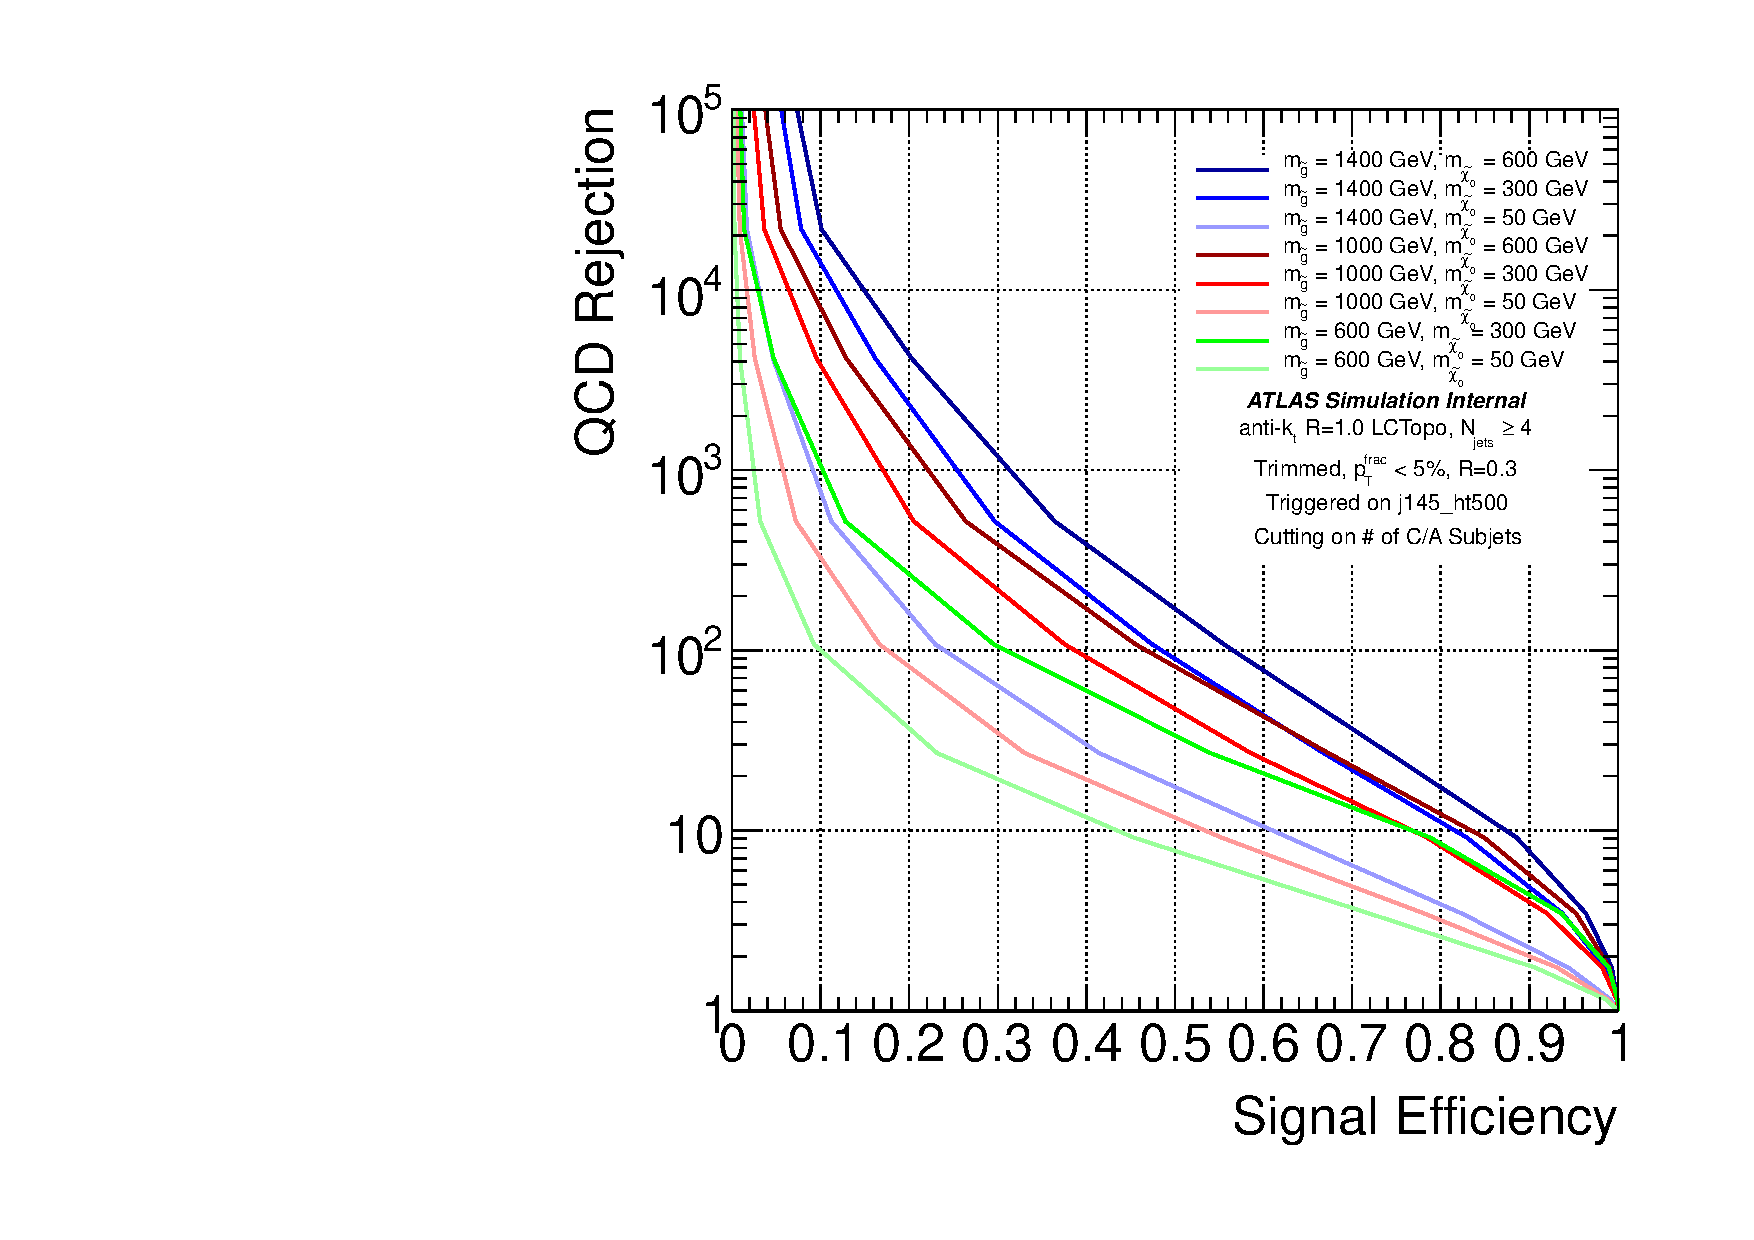
\includegraphics[width=0.45\textwidth]{INT/AntiKt10LCTopoTrimmedPtFrac5SmallR30_j145_ht500_NjetIncl_NFatJetMin4_NCASub4_g_RPVGluino}}
\label{fig:search:search:optimization:NCA}
\caption{Distribution of $N_{CA}$, a variable describing the total number of C/A subjets in the event. Several signal mass points and the \herwigpp di-jet background are shown. The right-hand plot shows the signal efficiency vs. background rejection of a scan of possible cuts on the $N_{CA}$ distribution.}
\end{figure}

%%%%%%%%%%%%%%%%%%%%%



%%%%%%%%%%%%%%%%%%%%%

\begin{figure}
\centering
\subfigure{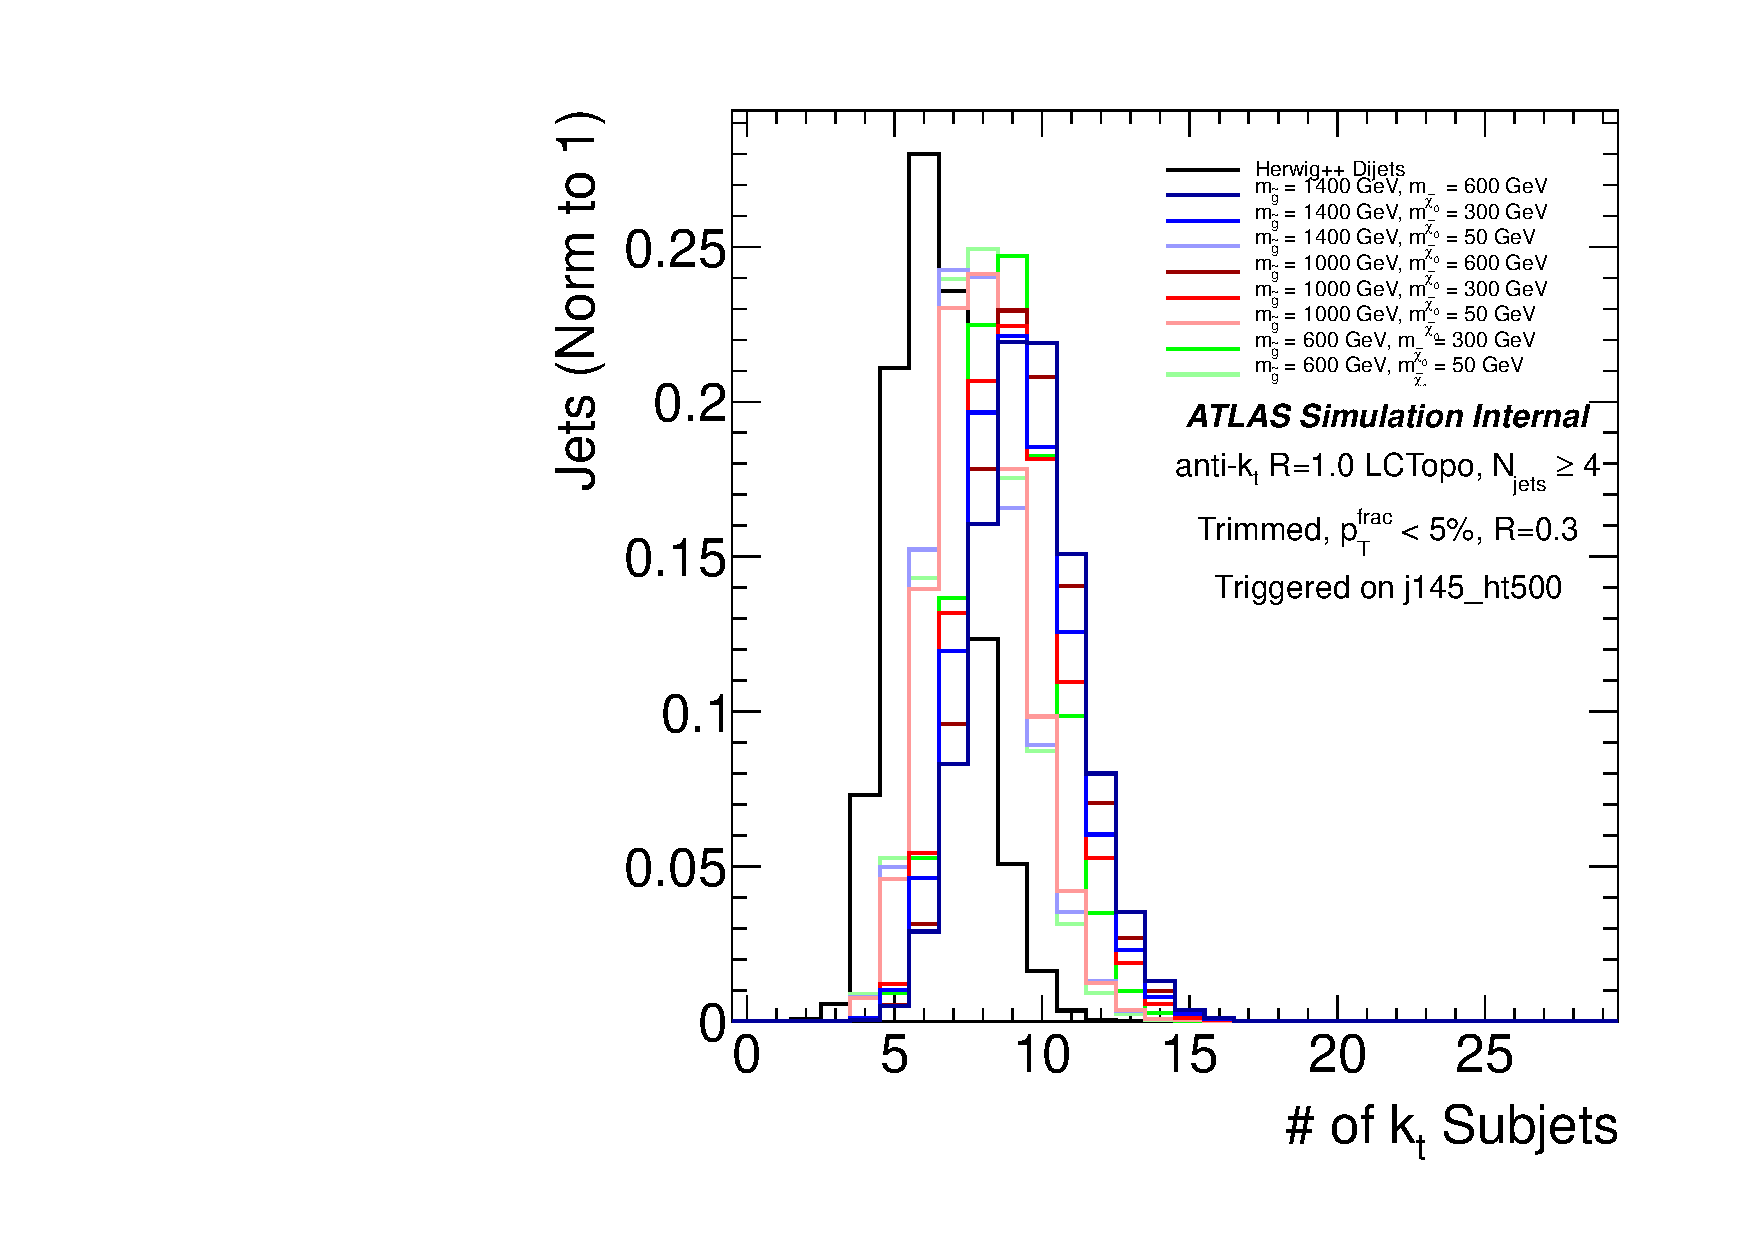
\includegraphics[width=0.45\textwidth]{INT/AntiKt10LCTopoTrimmedPtFrac5SmallR30_j145_ht500_NjetIncl_NFatJetMin4_NKTSub4_RPVGluino.pdf}}
\subfigure{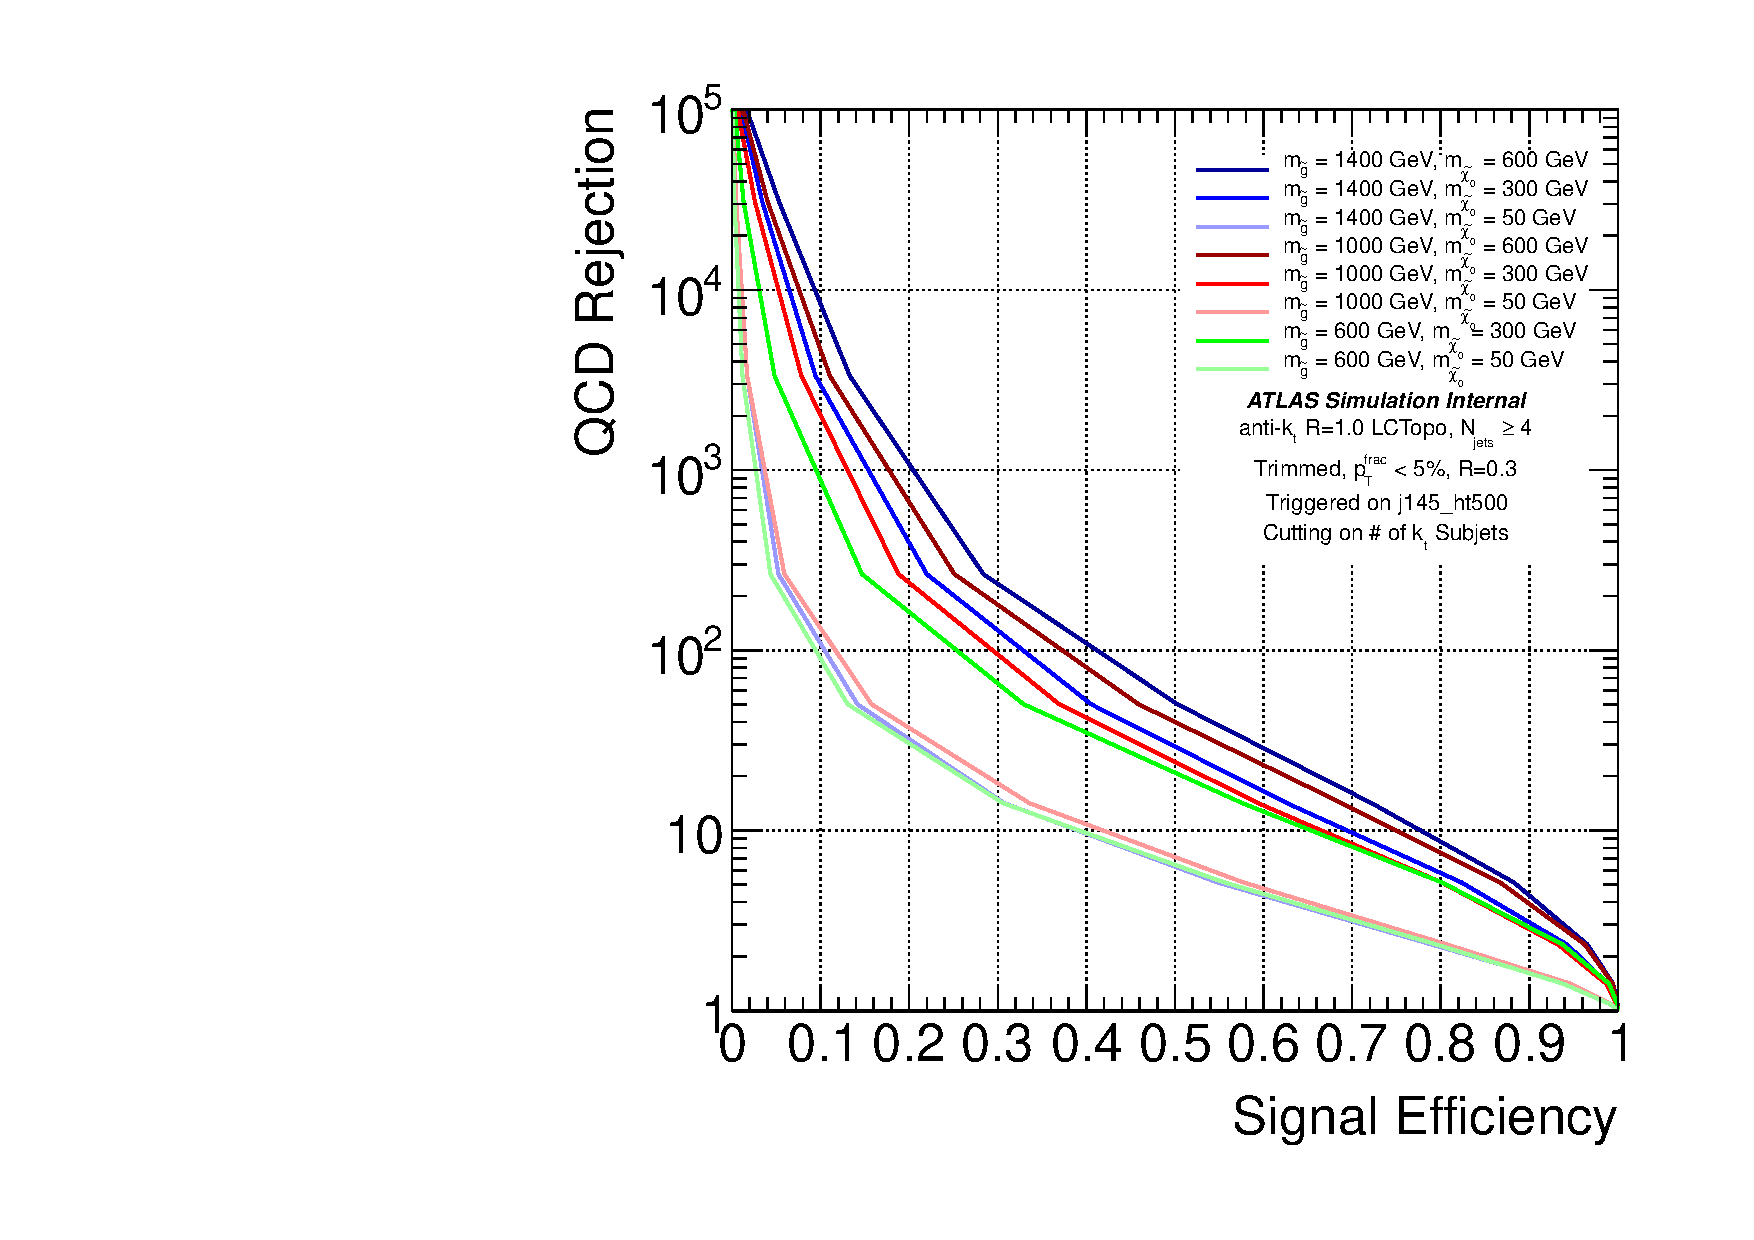
\includegraphics[width=0.45\textwidth]{INT/AntiKt10LCTopoTrimmedPtFrac5SmallR30_j145_ht500_NjetIncl_NFatJetMin4_NKTSub4_g_RPVGluino}}
\label{fig:search:search:optimization:NKT}
\caption{Distribution of $N_{kT}$, a variable describing the total number of \kt subjets in the event. Several signal mass points and the \herwigpp di-jet background are shown. The right-hand plot shows the signal efficiency vs. background rejection of a scan of possible cuts on the $N_{kT}$ distribution.}
\end{figure}

%%%%%%%%%%%%%%%%%%%%%




%%%%%%%%%%%%%%%%%%%%%

\begin{figure}
\centering
\subfigure{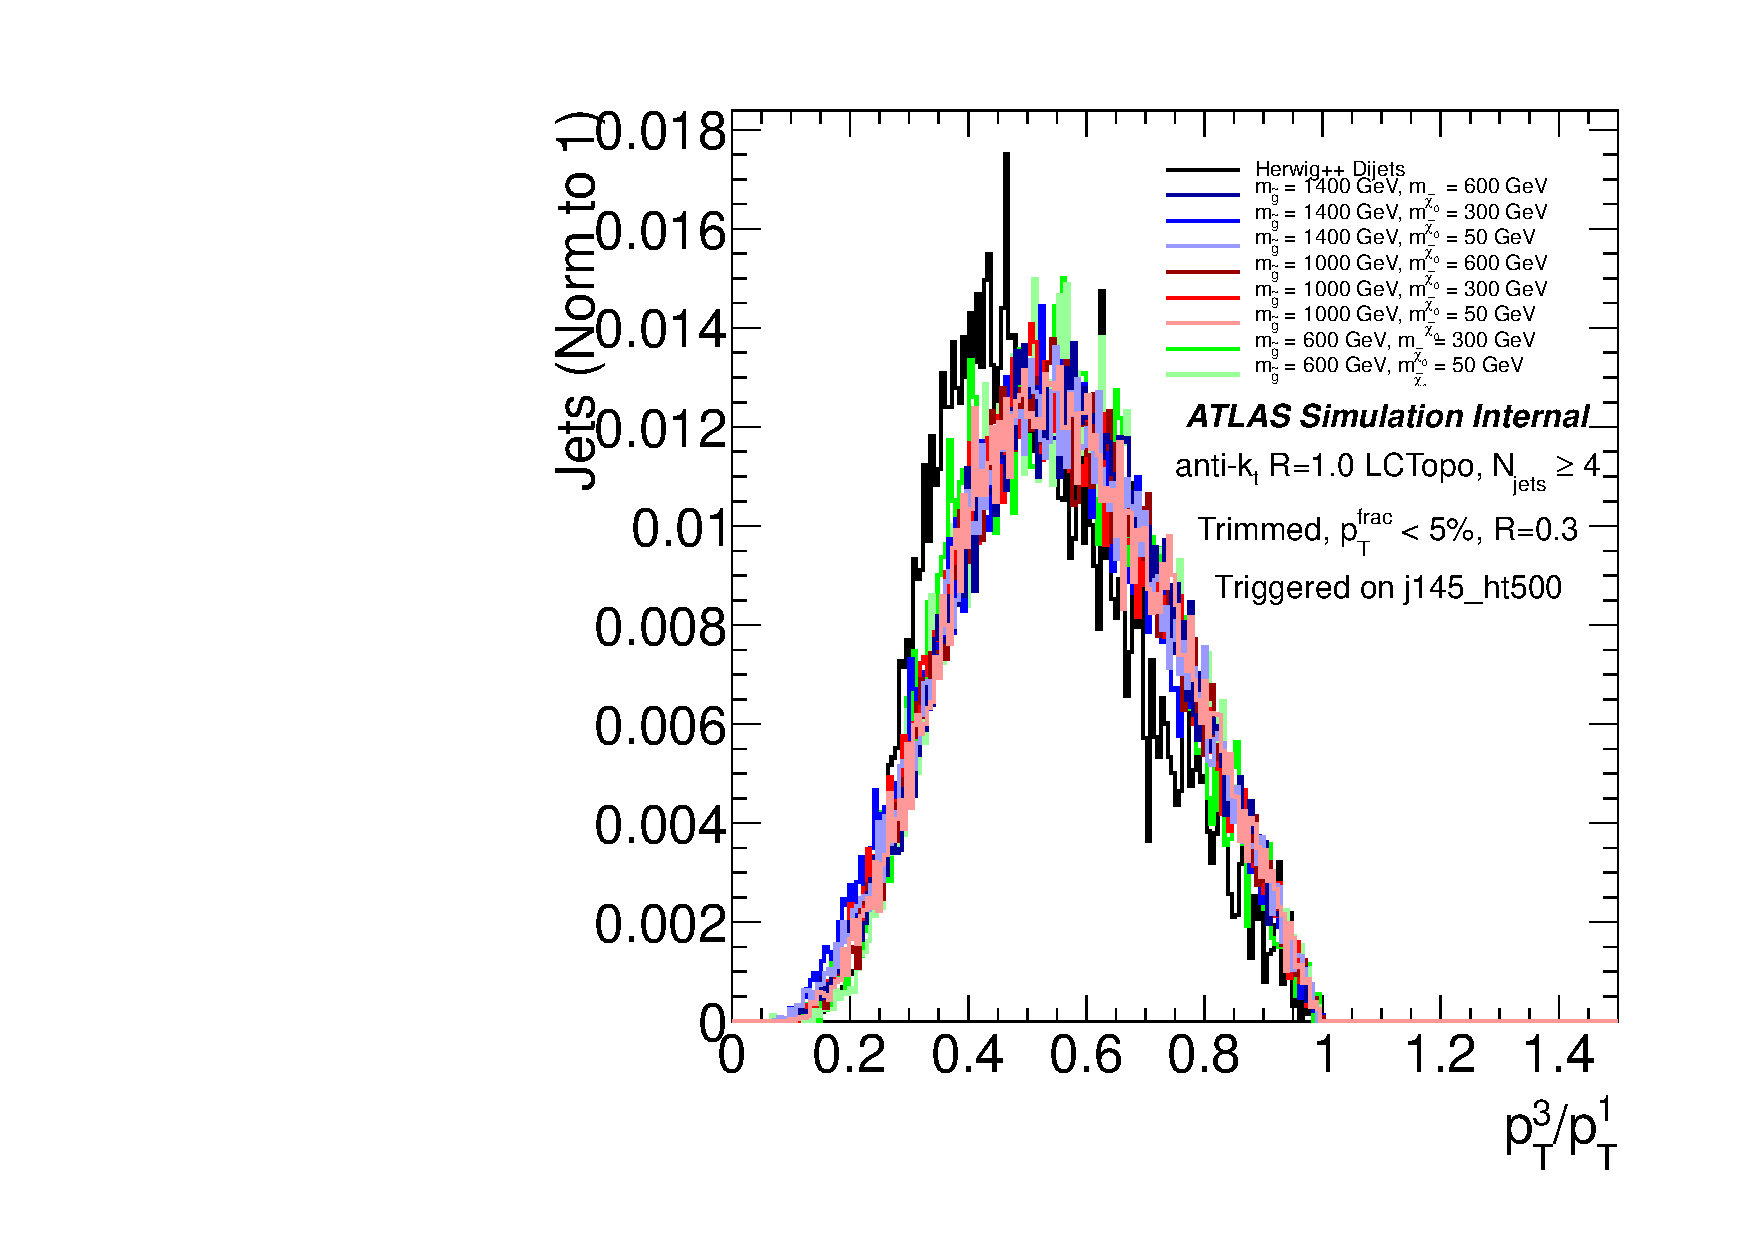
\includegraphics[width=0.45\textwidth]{INT/AntiKt10LCTopoTrimmedPtFrac5SmallR30_j145_ht500_NjetIncl_NFatJetMin4_PT31_RPVGluino.pdf}}
\subfigure{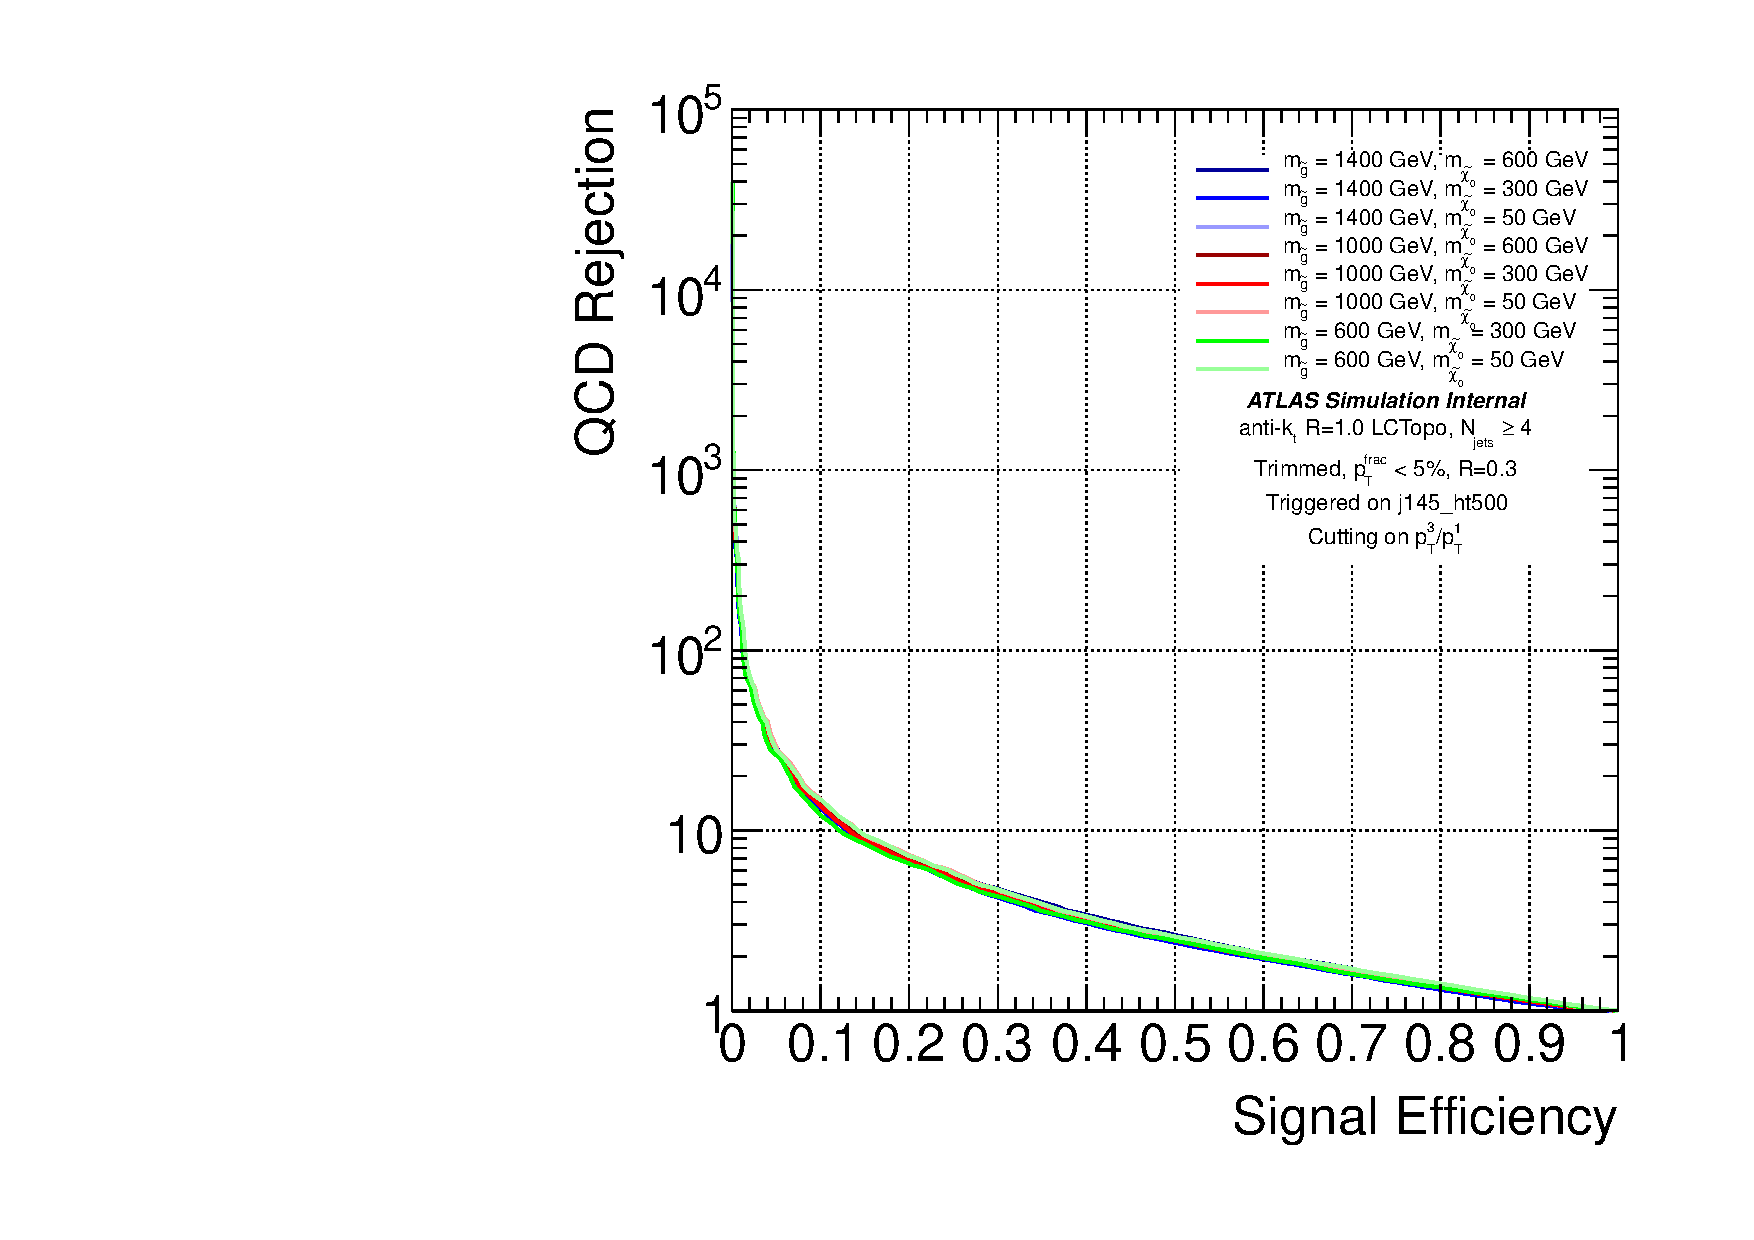
\includegraphics[width=0.45\textwidth]{INT/AntiKt10LCTopoTrimmedPtFrac5SmallR30_j145_ht500_NjetIncl_NFatJetMin4_PT31_g_RPVGluino}}
\label{fig:search:search:optimization:PT31}
\caption{Distribution of $\pt^3/\pt^1$, a variable describing the amount of energy in the third jet in the event. Several signal mass points and the \herwigpp di-jet background are shown. The right-hand plot shows the signal efficiency vs. background rejection of a scan of possible cuts on the $\pt^3/\pt^1$ distribution.}
\end{figure}

%%%%%%%%%%%%%%%%%%%%%


%%%%%%%%%%%%%%%%%%%%%

\begin{figure}
\centering
\subfigure{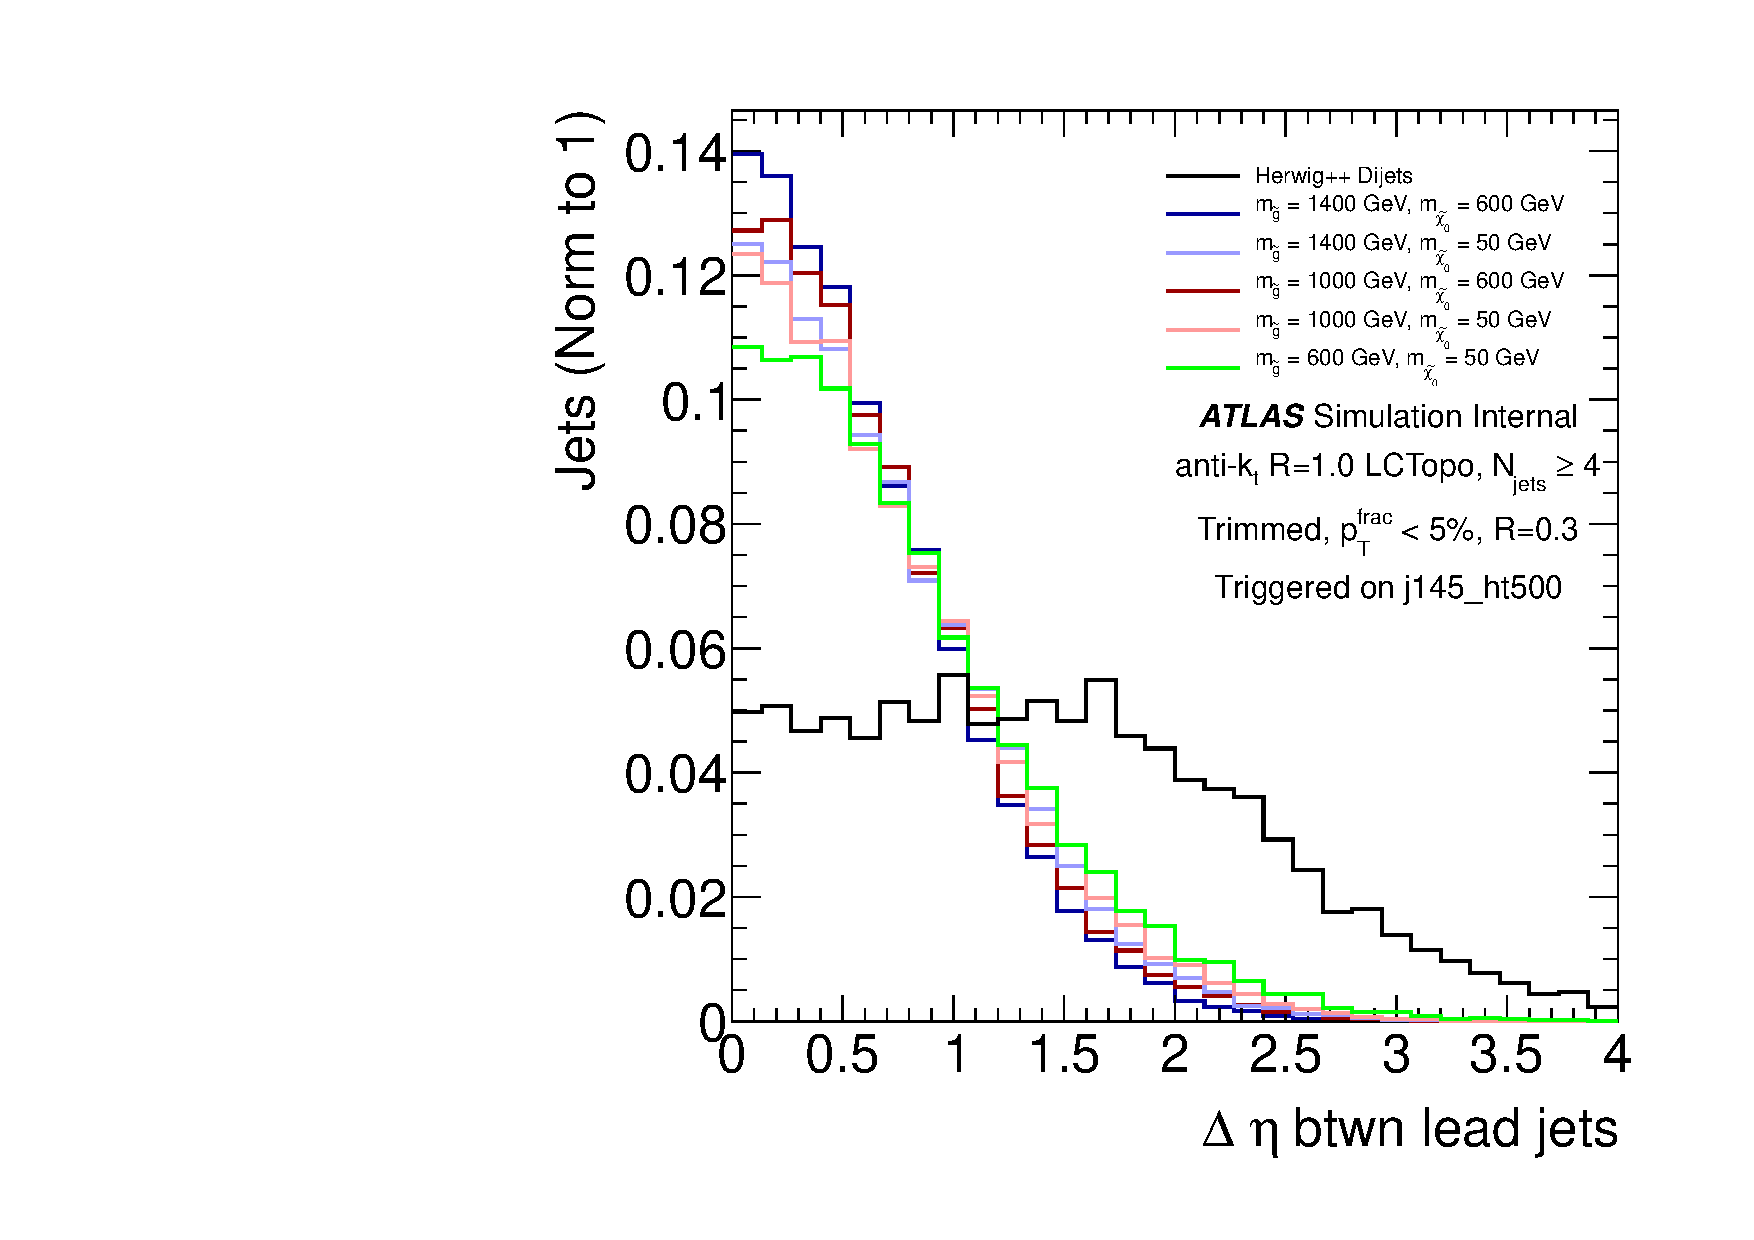
\includegraphics[width=0.45\textwidth]{INT/AntiKt10LCTopoTrimmedPtFrac5SmallR30_j145_ht500_NjetIncl_NFatJetMin4_DEta_RPVGluino.pdf}}
\subfigure{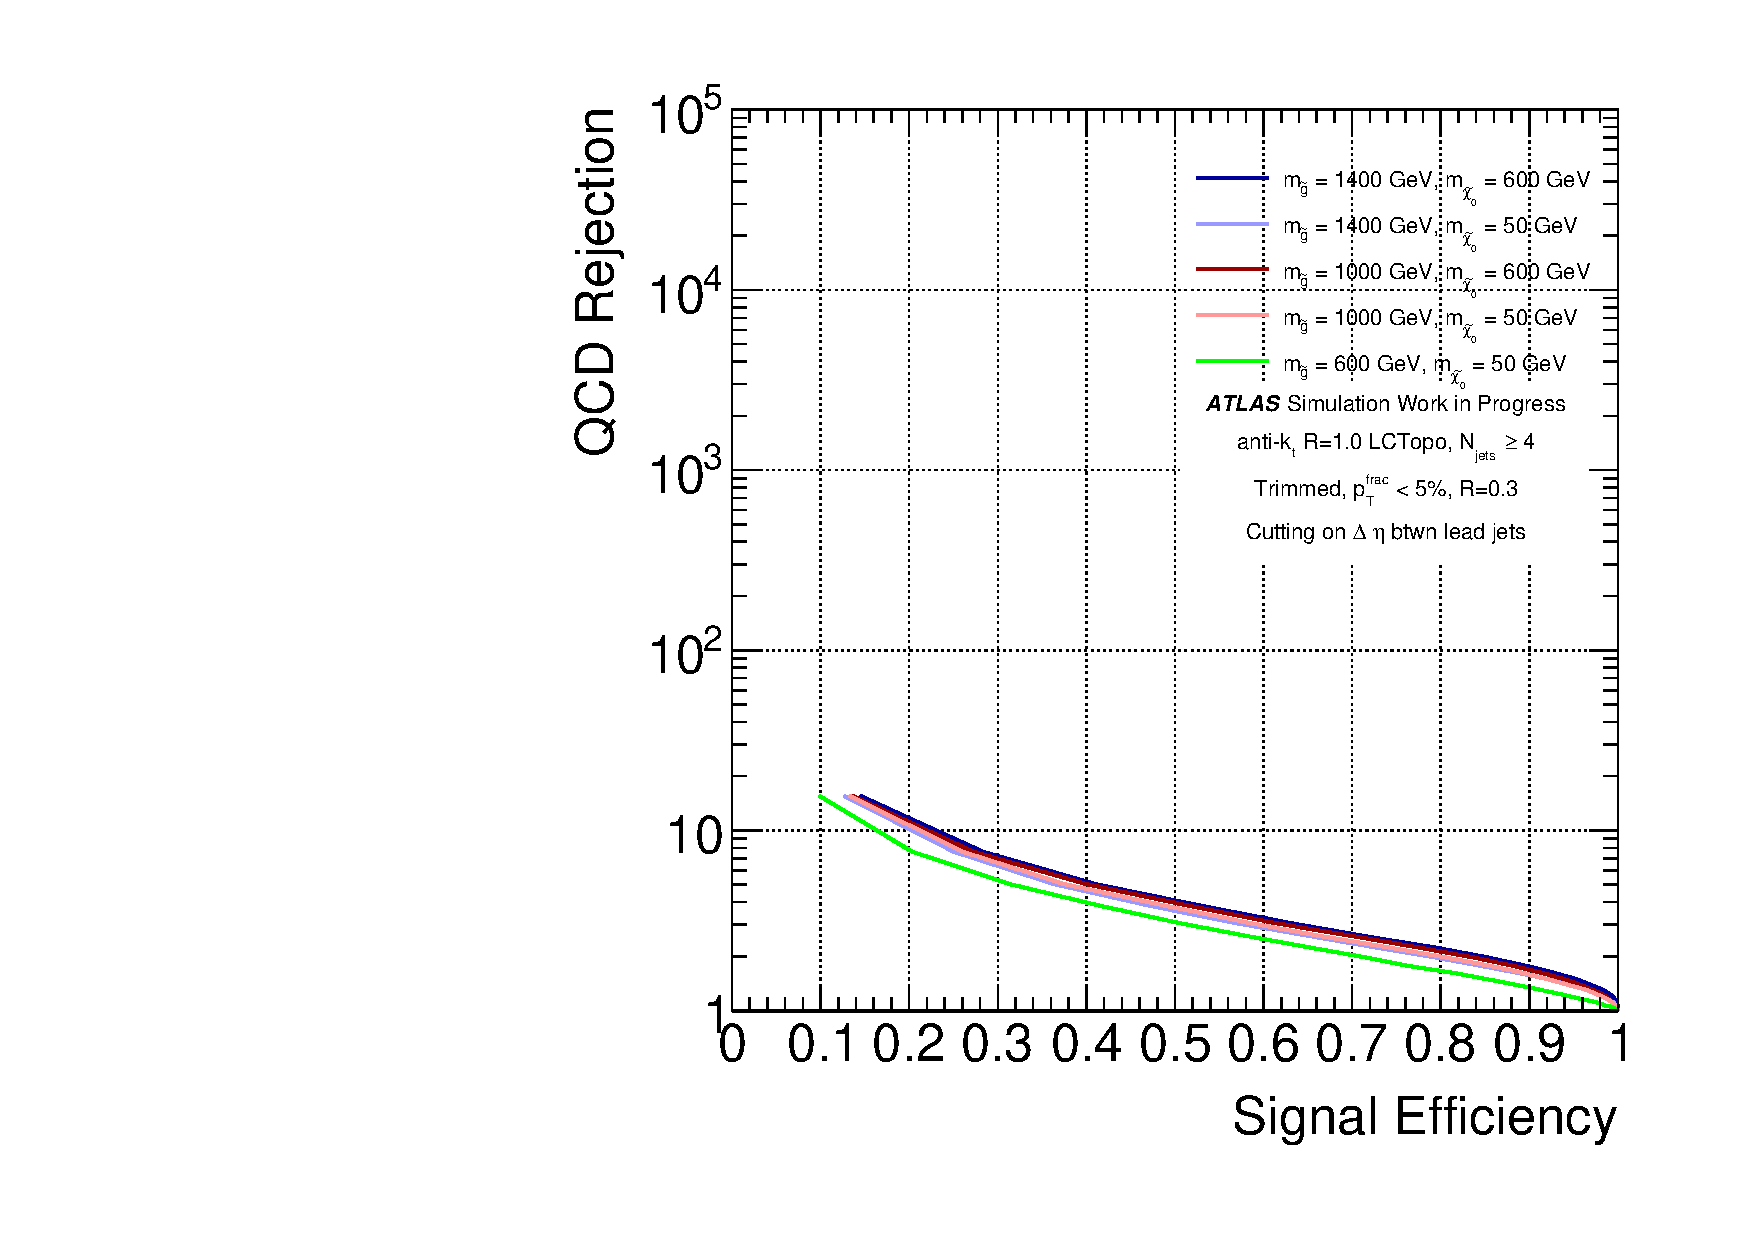
\includegraphics[width=0.45\textwidth]{INT/AntiKt10LCTopoTrimmedPtFrac5SmallR30_j360_a10_NjetIncl_NFatJetMin4_DEta_g_RPVGluino}}
\label{fig:search:search:optimization:DEta}
\caption{Distribution of $\Delta \eta$ a variable describing the difference in pseudo-rapidity between the leading two jets. Several signal mass points and the \herwigpp di-jet background are shown. The right-hand plot shows the signal efficiency vs. background rejection of a scan of possible cuts on the $\Delta \eta$ distribution.}
\end{figure}

%%%%%%%%%%%%%%%%%%%%%

Finally, Figure~\ref{fig:search:search:optimization:All} shows two efficiency vs. rejection curves for two different mass points, comparing all of the various variables previously shown (though $\Delta \eta$ is not shown, its performance is slightly stronger than $\pt^3/\pt^1$ on these plots). Several important conclusions are clear:

\begin{enumerate}
\item While \Ht is sometimes strongest at very high signal efficiency, and $N_{kT}$ and $N_{CA}$ sometimes strongest at very, very low signal efficiency, \MJ is generally the strongest variable by far.
\item \Ht is generally the second strongest variable, though it is a kinematic variable and so the background estimation may not work well with it.
\item $N_{kT}$ and $N_{CA}$ generally work very well-- but integer type variables may be problematic with a Gaussian kernel smoothing.
\item $T_{32}$ and $T_{21}$ perform worse than the subjet counting variables, but do have some power.
\item $\pt^3/\pt^1$ has comparatively low power.
\end{enumerate}

%%%%%%%%%%%%%%%%%%%%%

\begin{figure}
\centering
\subfigure{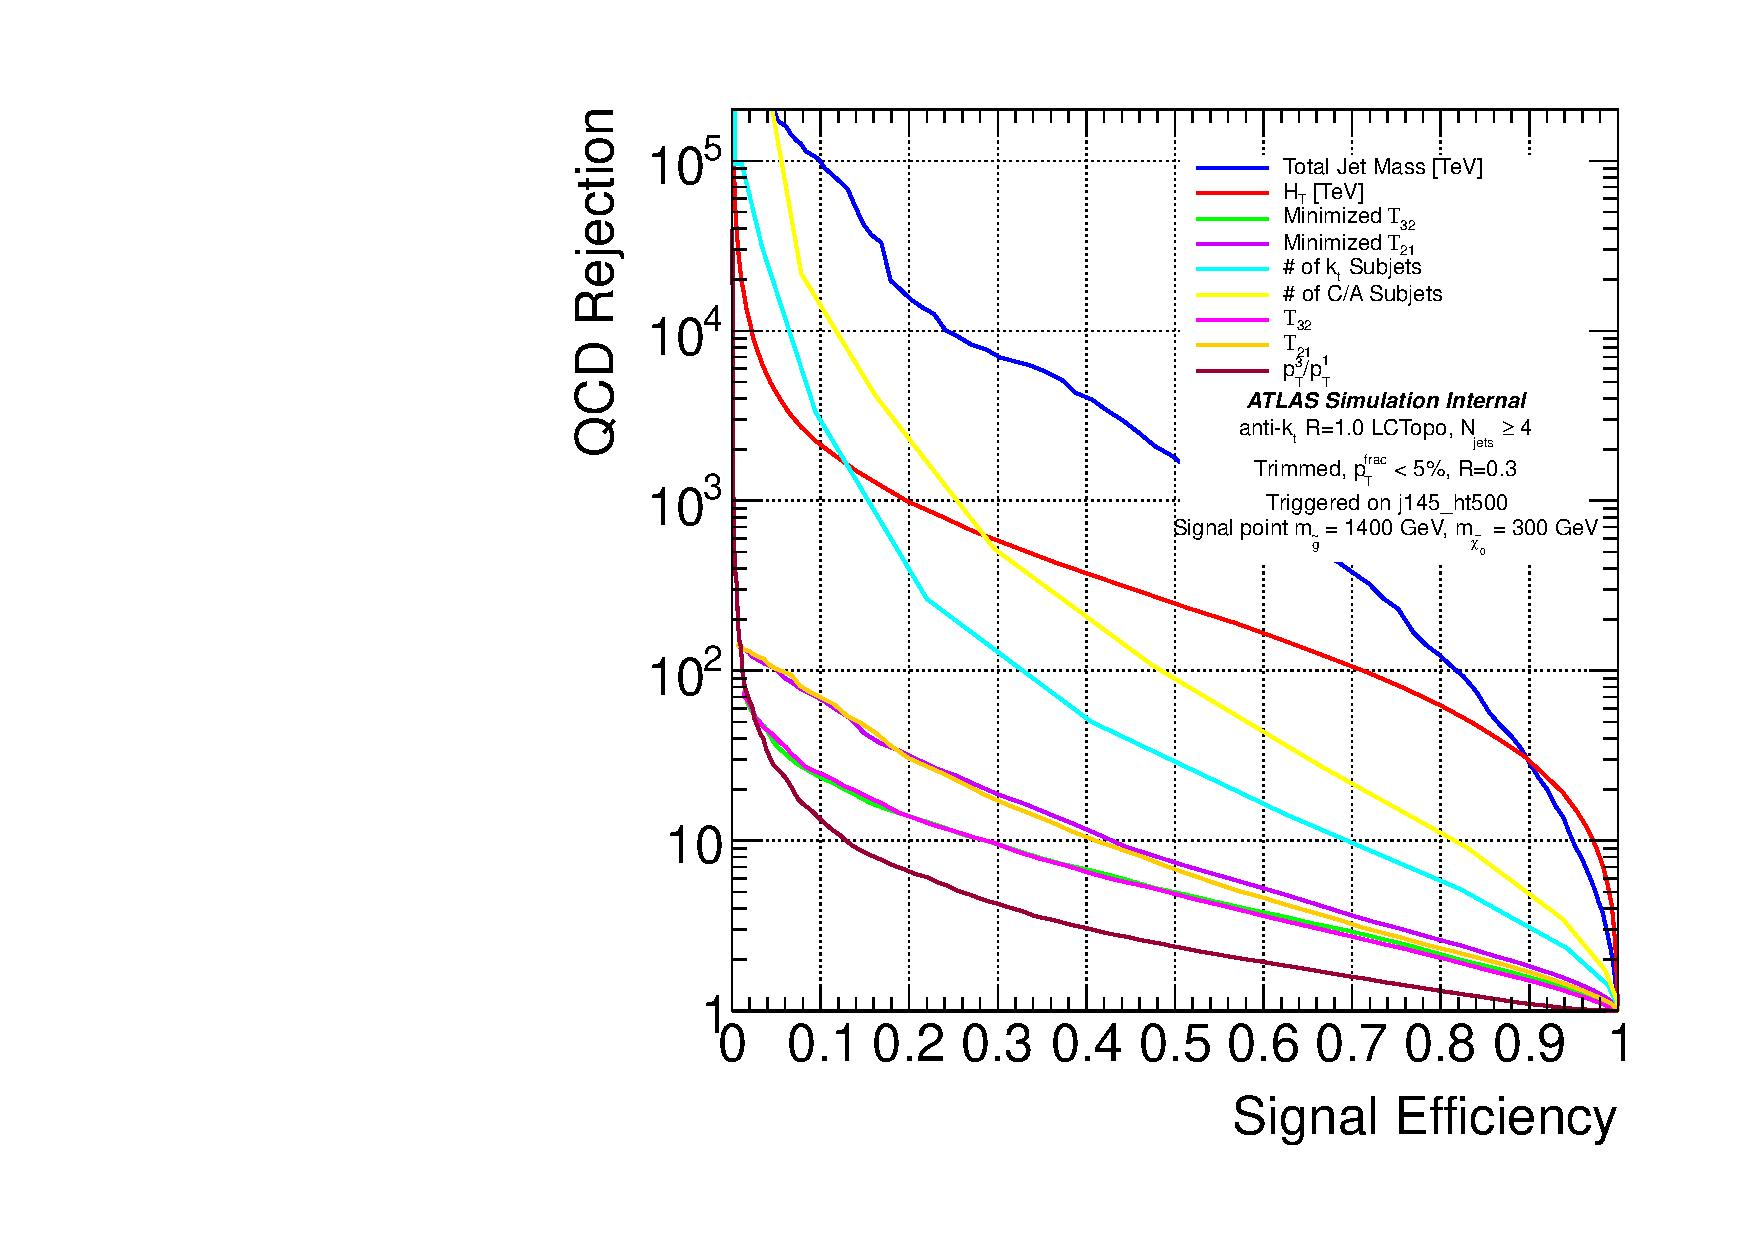
\includegraphics[width=0.45\textwidth]{INT/AntiKt10LCTopoTrimmedPtFrac5SmallR30_j145_ht500_NjetIncl_NFatJetMin4_SigPoint2_g_RPVGluino}}
\subfigure{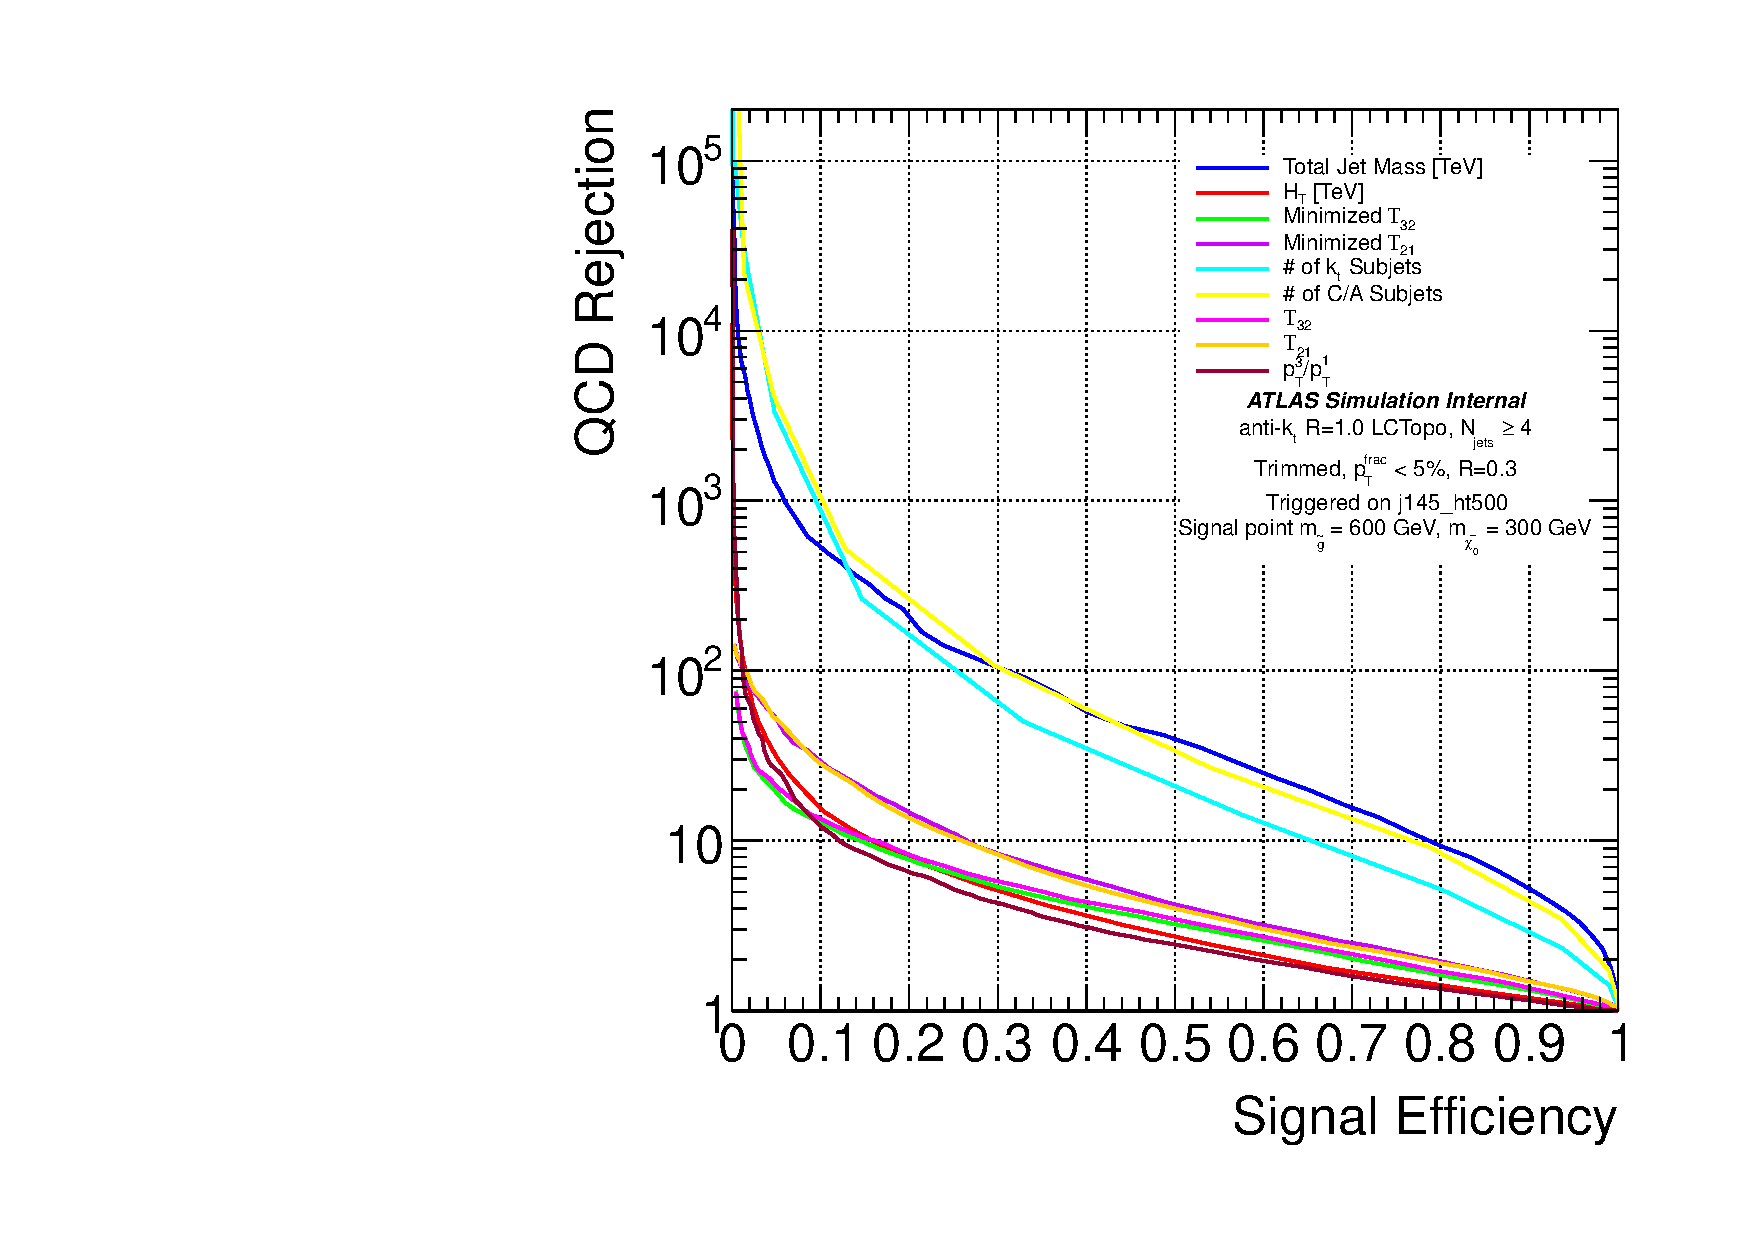
\includegraphics[width=0.45\textwidth]{INT/AntiKt10LCTopoTrimmedPtFrac5SmallR30_j145_ht500_NjetIncl_NFatJetMin4_SigPoint7_g_RPVGluino}}
\label{fig:search:search:optimization:All}
\caption{Signal efficiency vs. background rejection curves for two pass points, comparing the power of various variables. $\Delta \eta$ is not shown, but has similar power (though slightly stronger) than $\pt^3 / \pt^1$.}
\end{figure}

%%%%%%%%%%%%%%%%%%%%%

From this set of results, it is clear that \MJ is a good candidate for a final discriminant variable which can apply the most discrimination between signal and background. There are several other candidates for the second variable used for defining signal and control regions, but these need two-dimensional correlation studies in order to understand the best pairing.

Throughout these studies, the event-level variables have been constructed from the leading 4 jets (recall that the signal region was pre-selected to have $>=4$ jets. Other possibilities-- such as constructing the substructure observable from only the leading 2 jets-- could potentially make the background estimation easier, but come at a price of slightly reduced discrimination (as the third and fourth jets do have useful substructure information to contribute). Similarly, one could add more jets to the sums/means if they existed, but this was found to not contribute at all to discrimation, and as it would further complicate the background estimation, this strategy was not adopted. For this reasons, all the variables considered simply use the leading 4 jets in the event.

One important consideration, for the sake of the background estimation, is understanding whether the \pt spectrum is sensitive to new physics (as we use the \pt spectrum to determine the background expectation). Figure~\ref{fig:search:search:optimization:pt} shows that the \pt spectrum is essentially unchanged, showing that we can use the kinematics without worry of biasing the background estimate.

%%%%%%%%%%%%%%%%

\begin{figure}
\centering
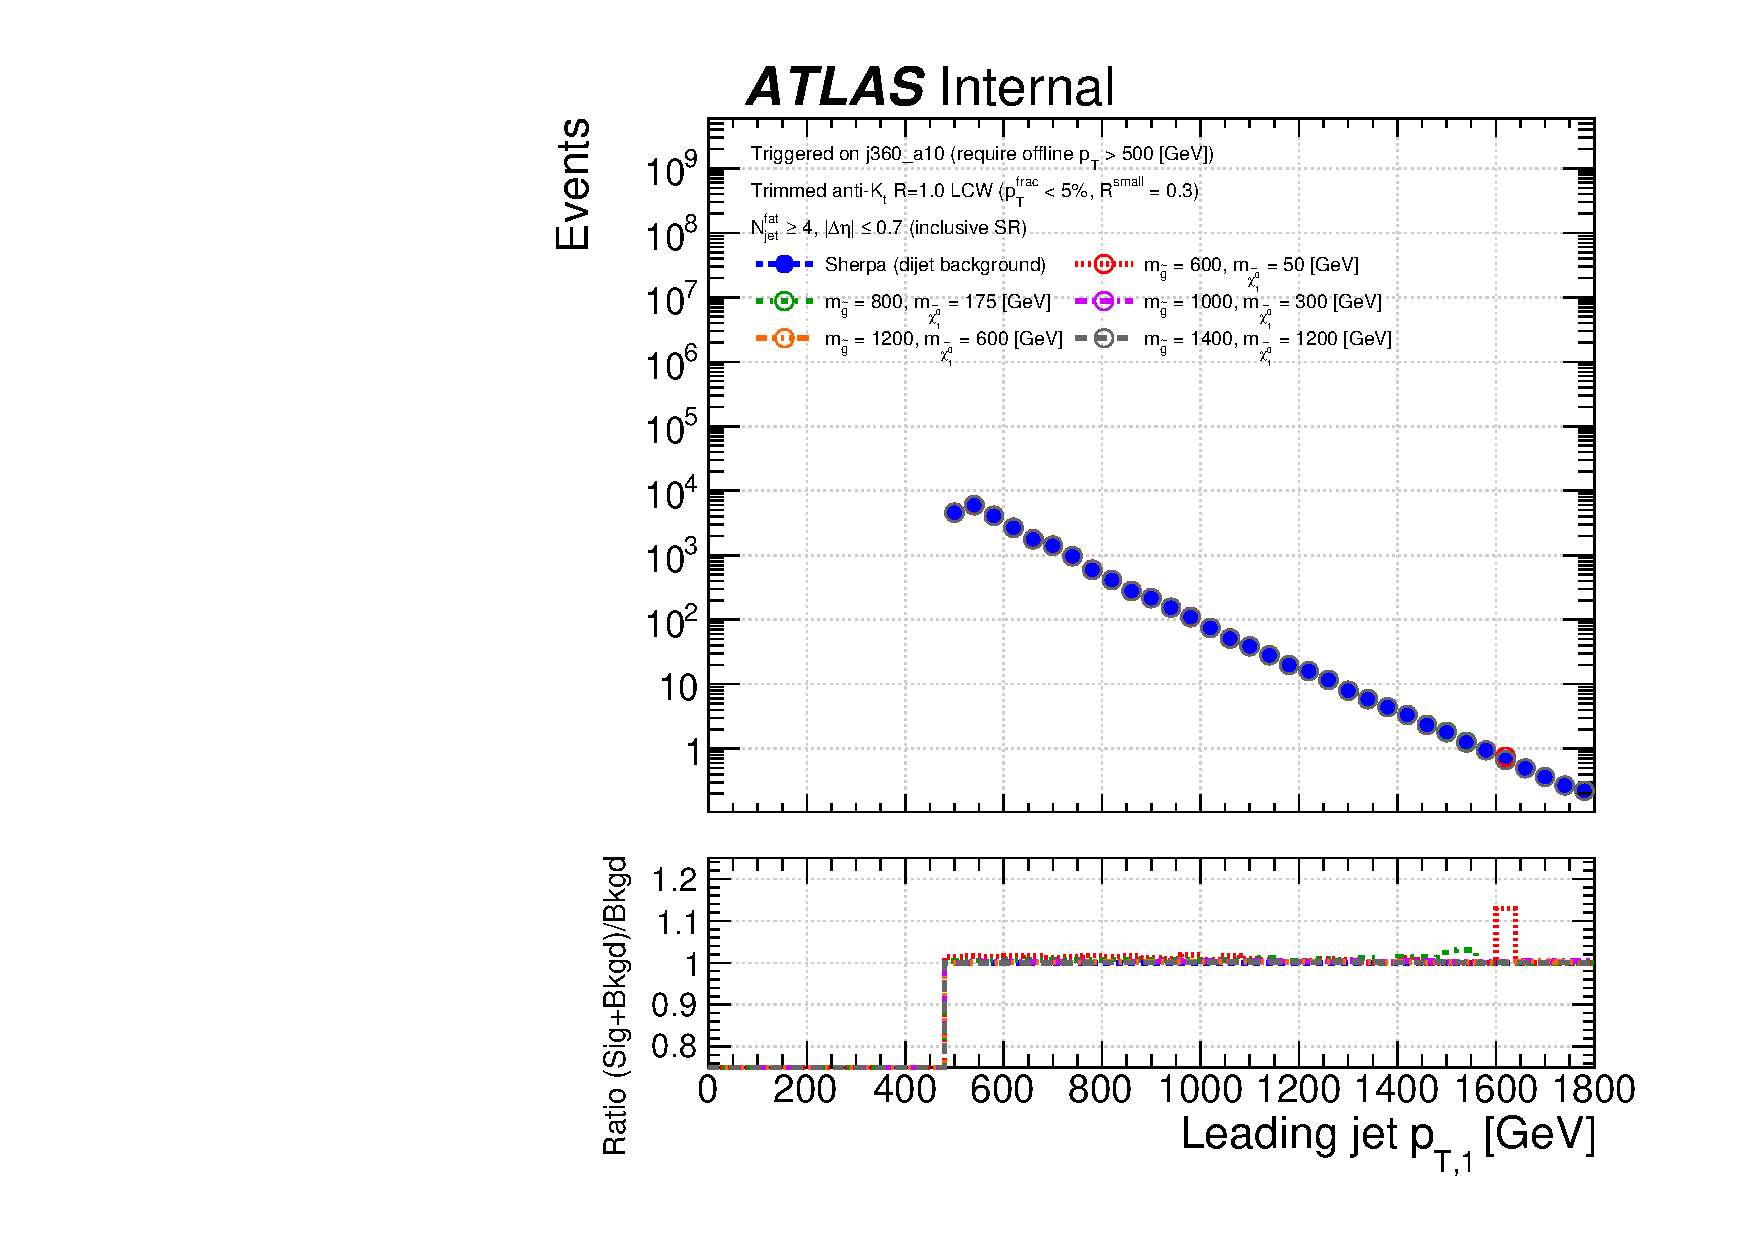
\includegraphics[width=0.5\textwidth]{INT/overlay_sigBkgd_sherpaDijets_logy_stacked_jet_pT1_NFatJetMin4_lowDEta70incl_CR_AntiKt10LCTopoTrimmedPtFrac5SmallR30.pdf}
\label{fig:search:search:optimization:pt}
\caption{An example of a \pt distribution for the leading jet, using \Sherpa multi-jet backgrounds, with various signal models overlaid.}
\end{figure}


\subsubsection{Additional 1D Studies}

Additionally, one could ask whether individual jet masses are useful for signal discrimination. Figures~\ref{fig:search:search:optimization:signalcomp1} and \ref{fig:search:search:optimization:signalcomp2} show the leading and subleading mass distribution as compared to \Herwigpp backgrounds: the important thing to notice is that for no signal point is the mass of the $\tilde{g}$, or the mass of the \lsp, properly and consistently reconstructed. This demonstrates the advantage of the accidental substructure approach: for such a complicated signal, the significant overlaps between various decay products mean it is easiest to simply use the mass as a discriminant, without trying to reconstruct a specific particle's mass.


%%------------------------------    

\begin{figure}[!ht]
  \centering
  
  \subfigure[High boost mass points.]{
    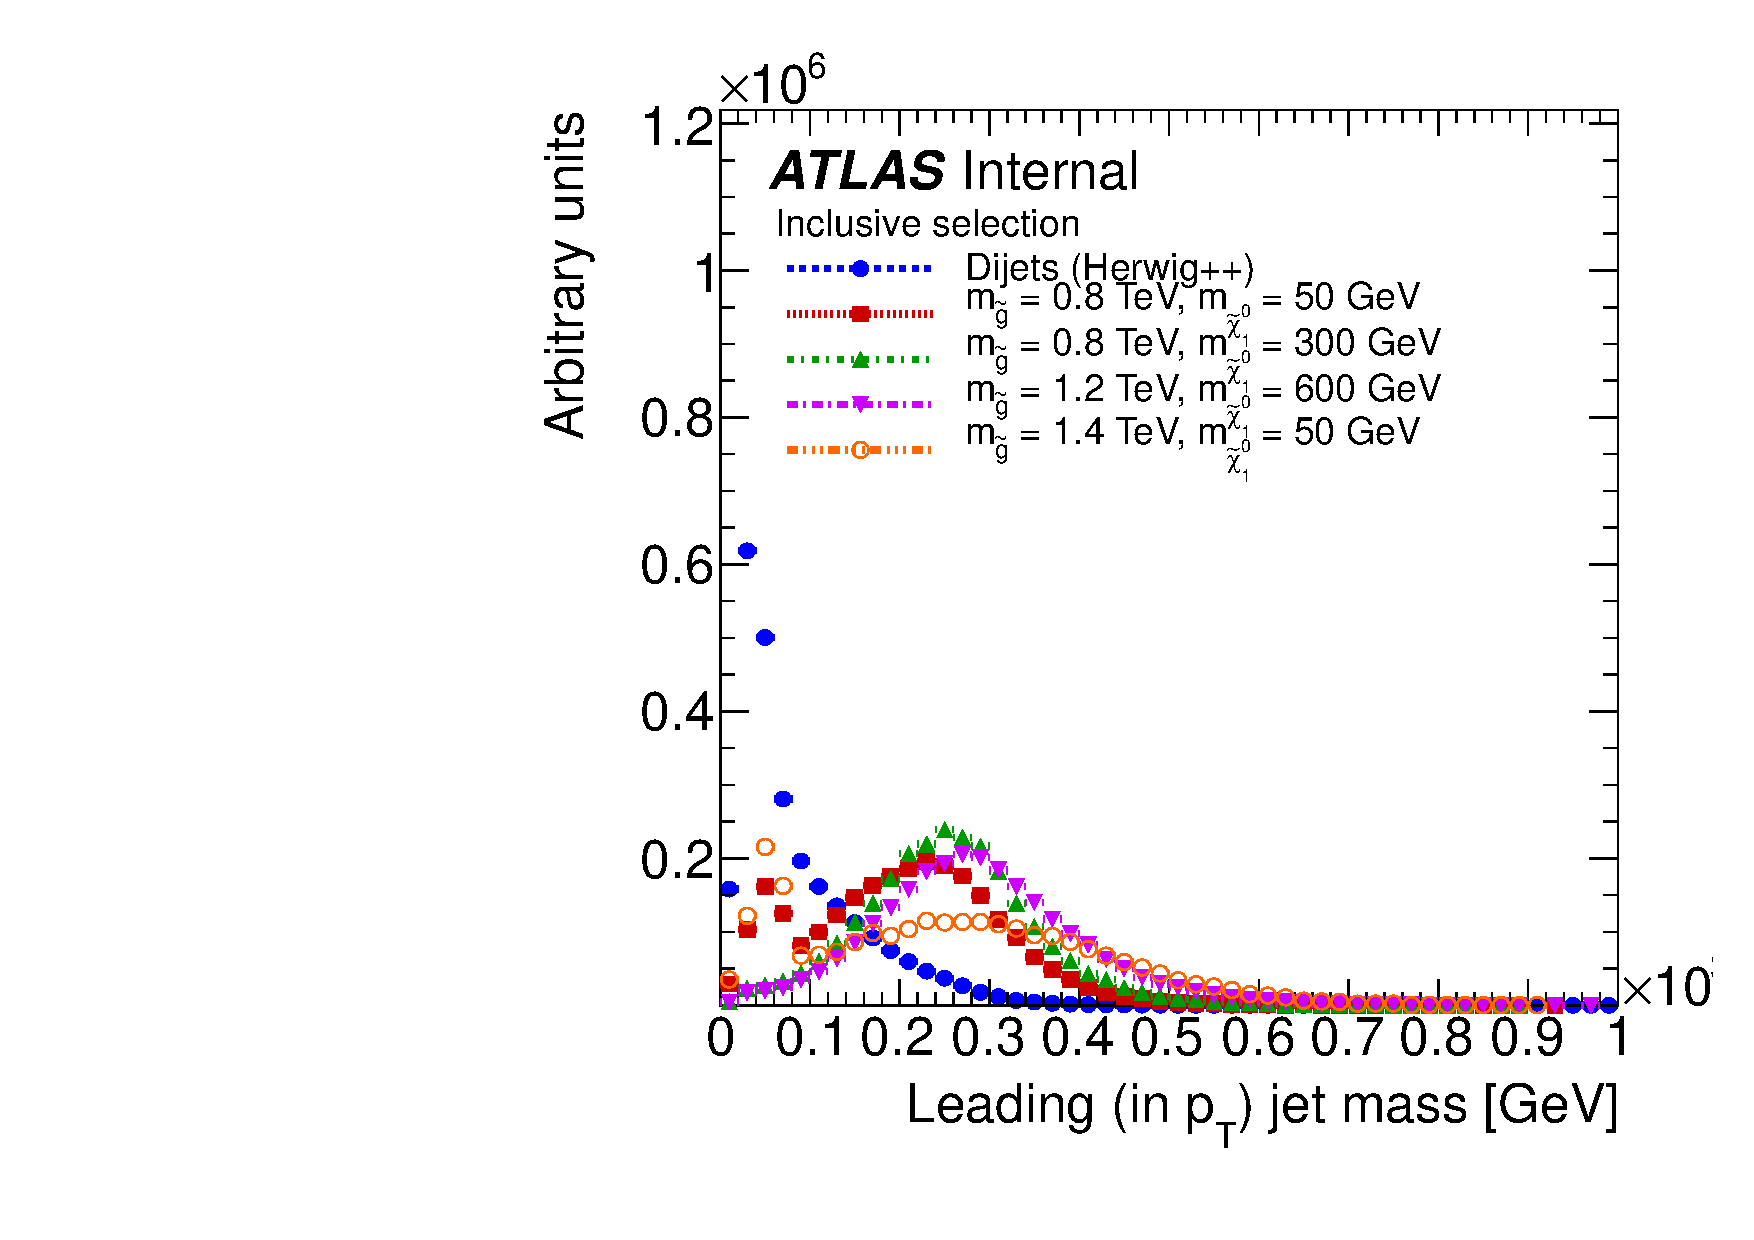
\includegraphics[width=0.45\columnwidth]{INT/Discrimination/overlay_jet_mass1_signalComparison_highBoost_Incl_j470_AntiKt10LCTopoTrimmedPtFrac5SmallR30_data12_v22.pdf}
    \label{fig:search:search:optimization:signalcomp1:highboost}}~
  \subfigure[High $\mgluino$ mass points]{
    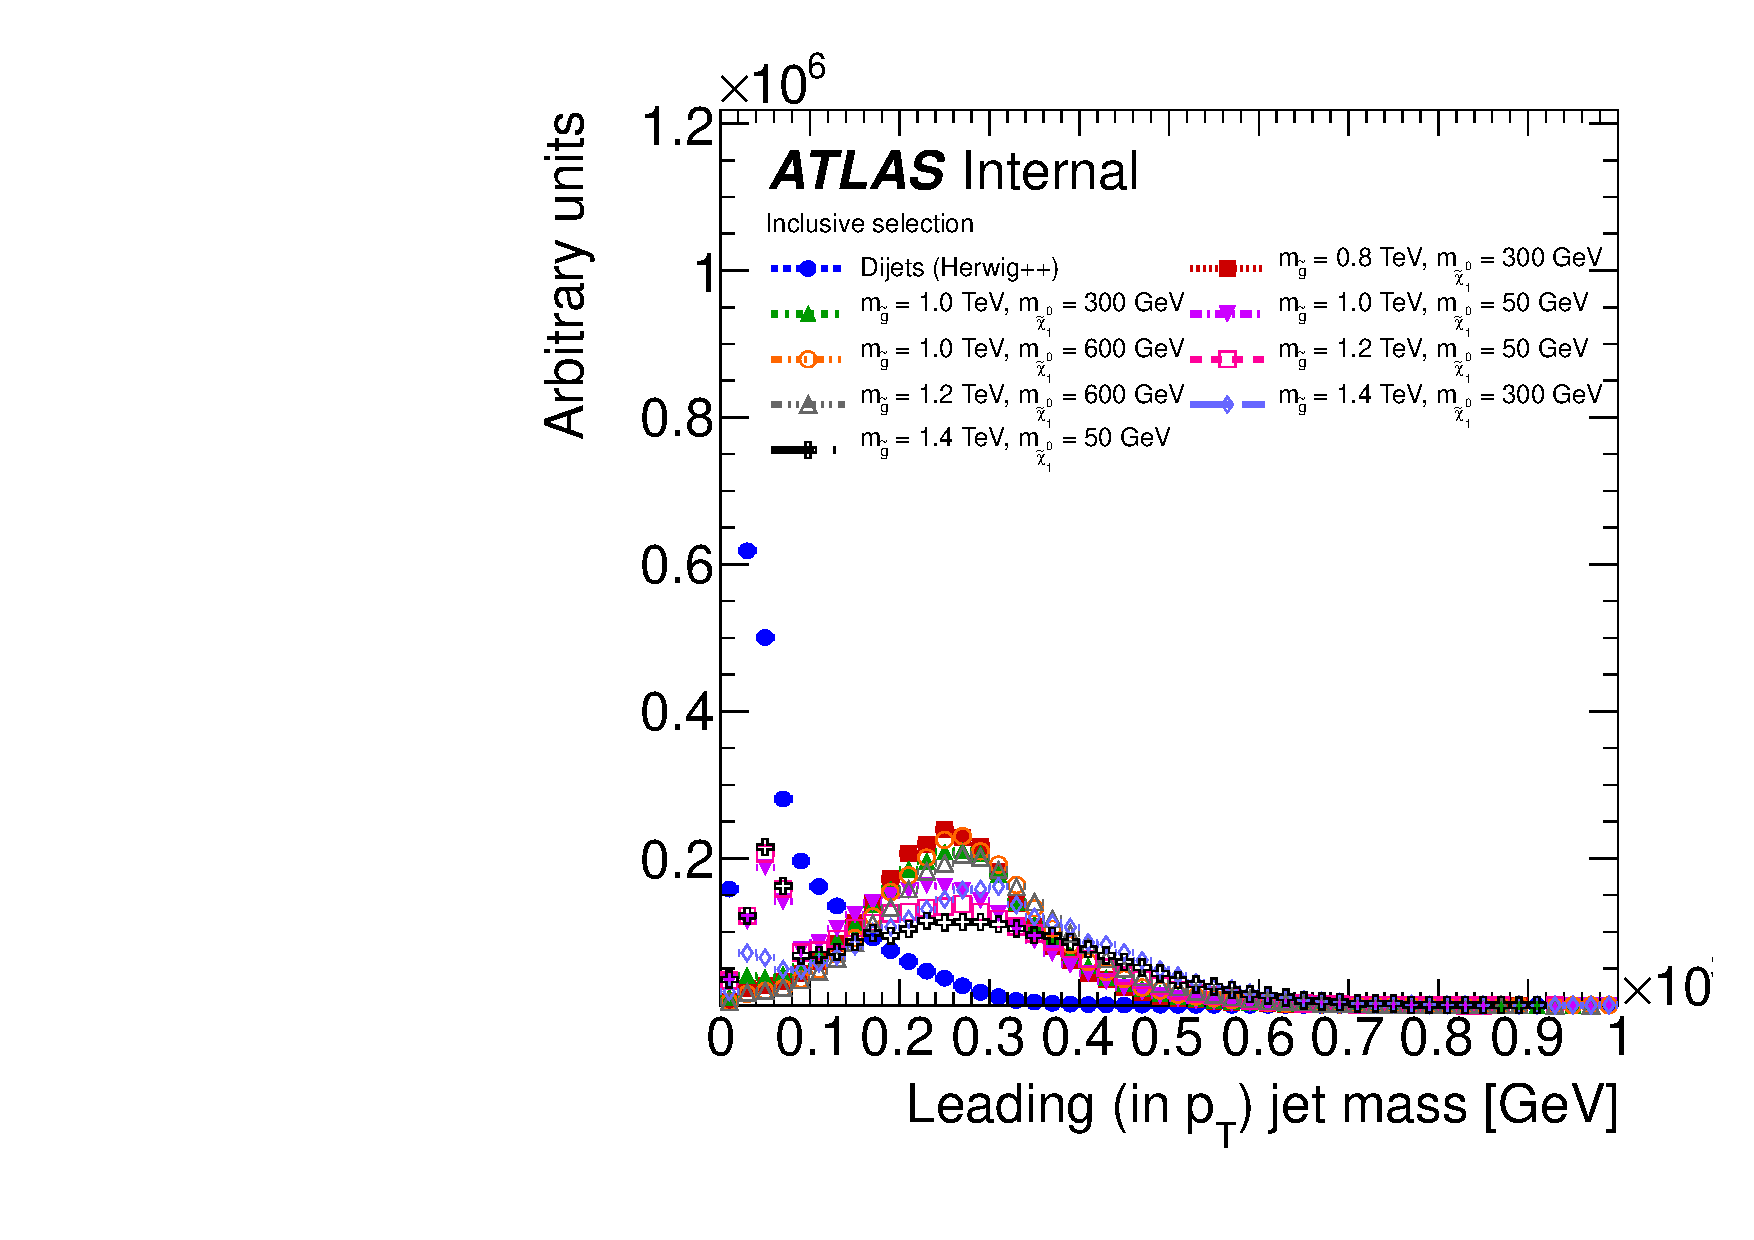
\includegraphics[width=0.45\columnwidth]{INT/Discrimination/overlay_jet_mass1_signalComparison_highGluinoM_Incl_j470_AntiKt10LCTopoTrimmedPtFrac5SmallR30_data12_v22.pdf}
    \label{fig:search:search:optimization:signalcomp1:highmg}}
  \subfigure[$\mgluino = 1$ TeV mass points]{
    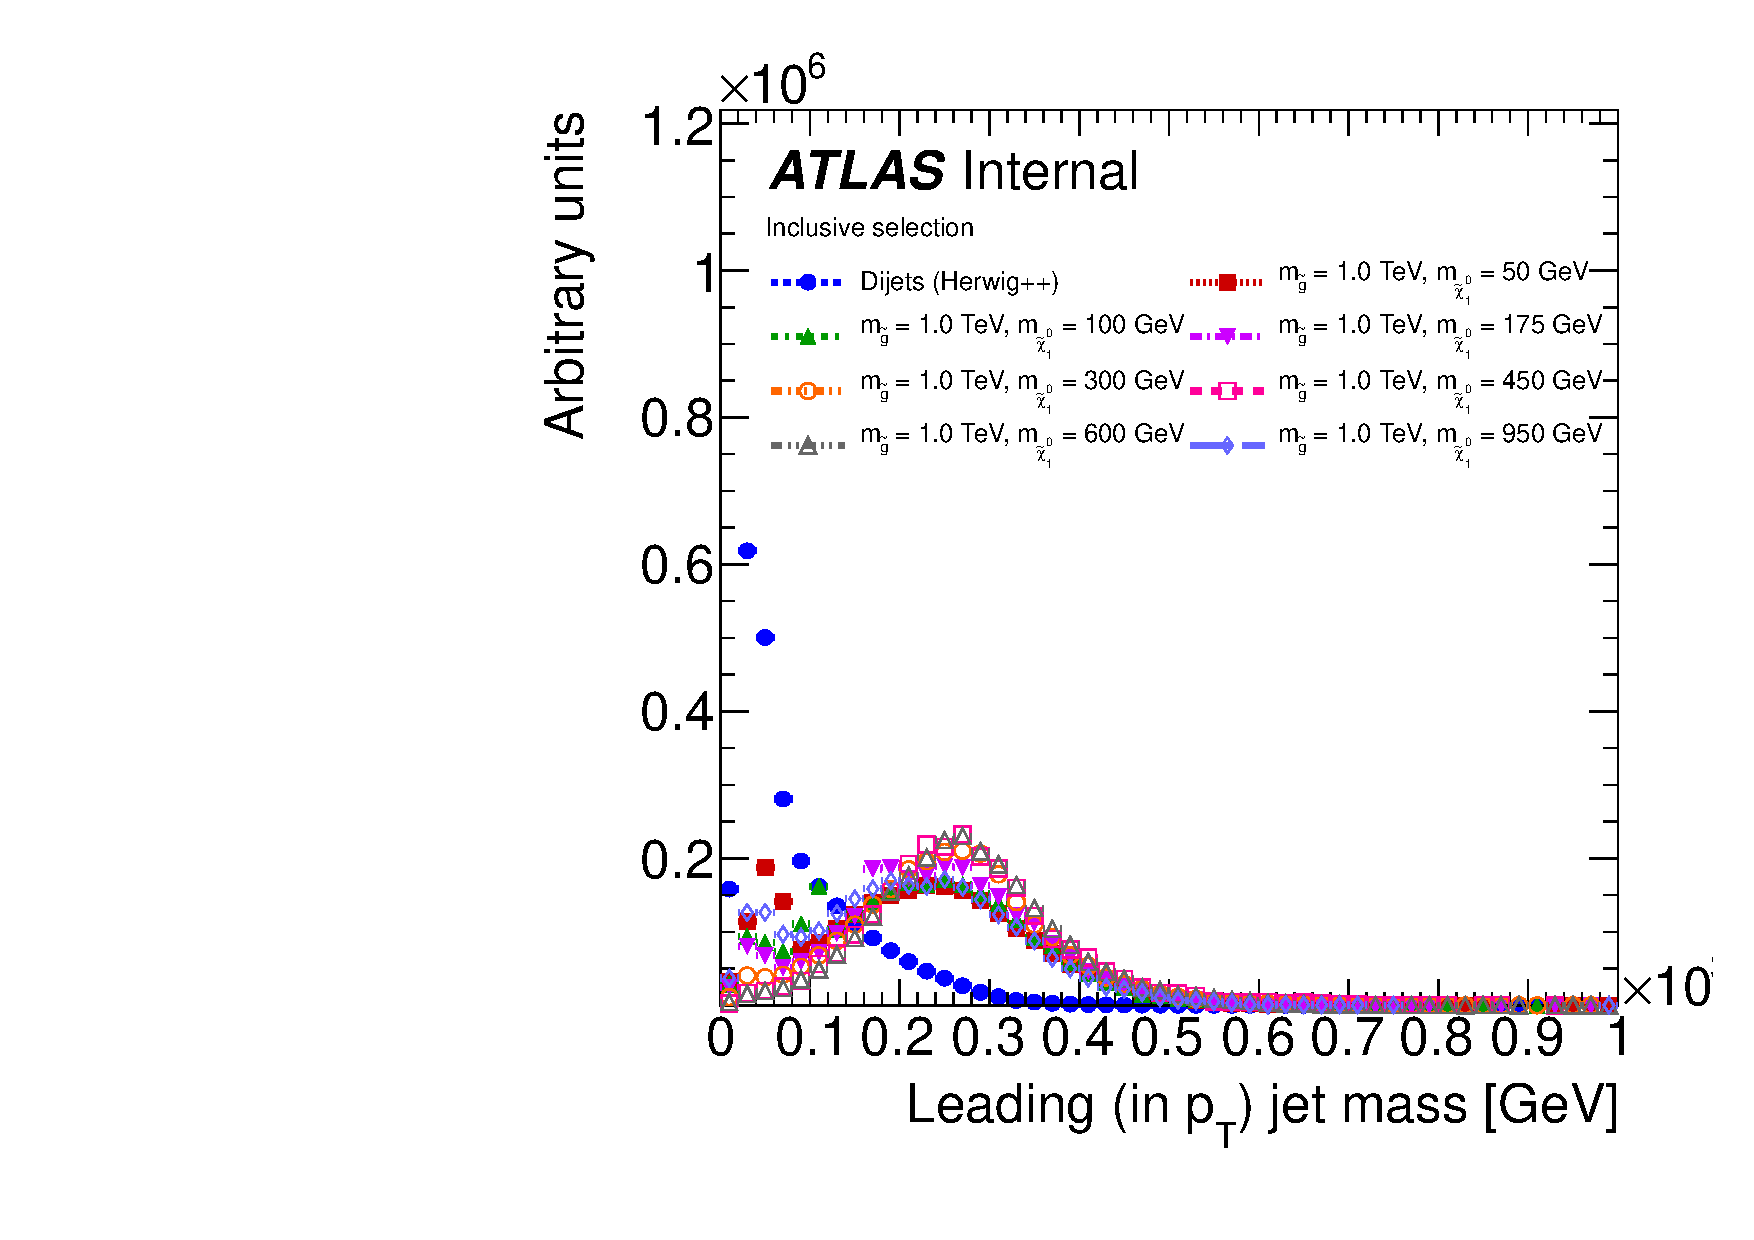
\includegraphics[width=0.45\columnwidth]{INT/Discrimination/overlay_jet_mass1_signalComparison_OneTeV_Incl_j470_AntiKt10LCTopoTrimmedPtFrac5SmallR30_data12_v22.pdf}~
    \label{fig:search:search:optimization:signalcomp1:tevmg}}
  \subfigure[$\sim$Top mass points]{
    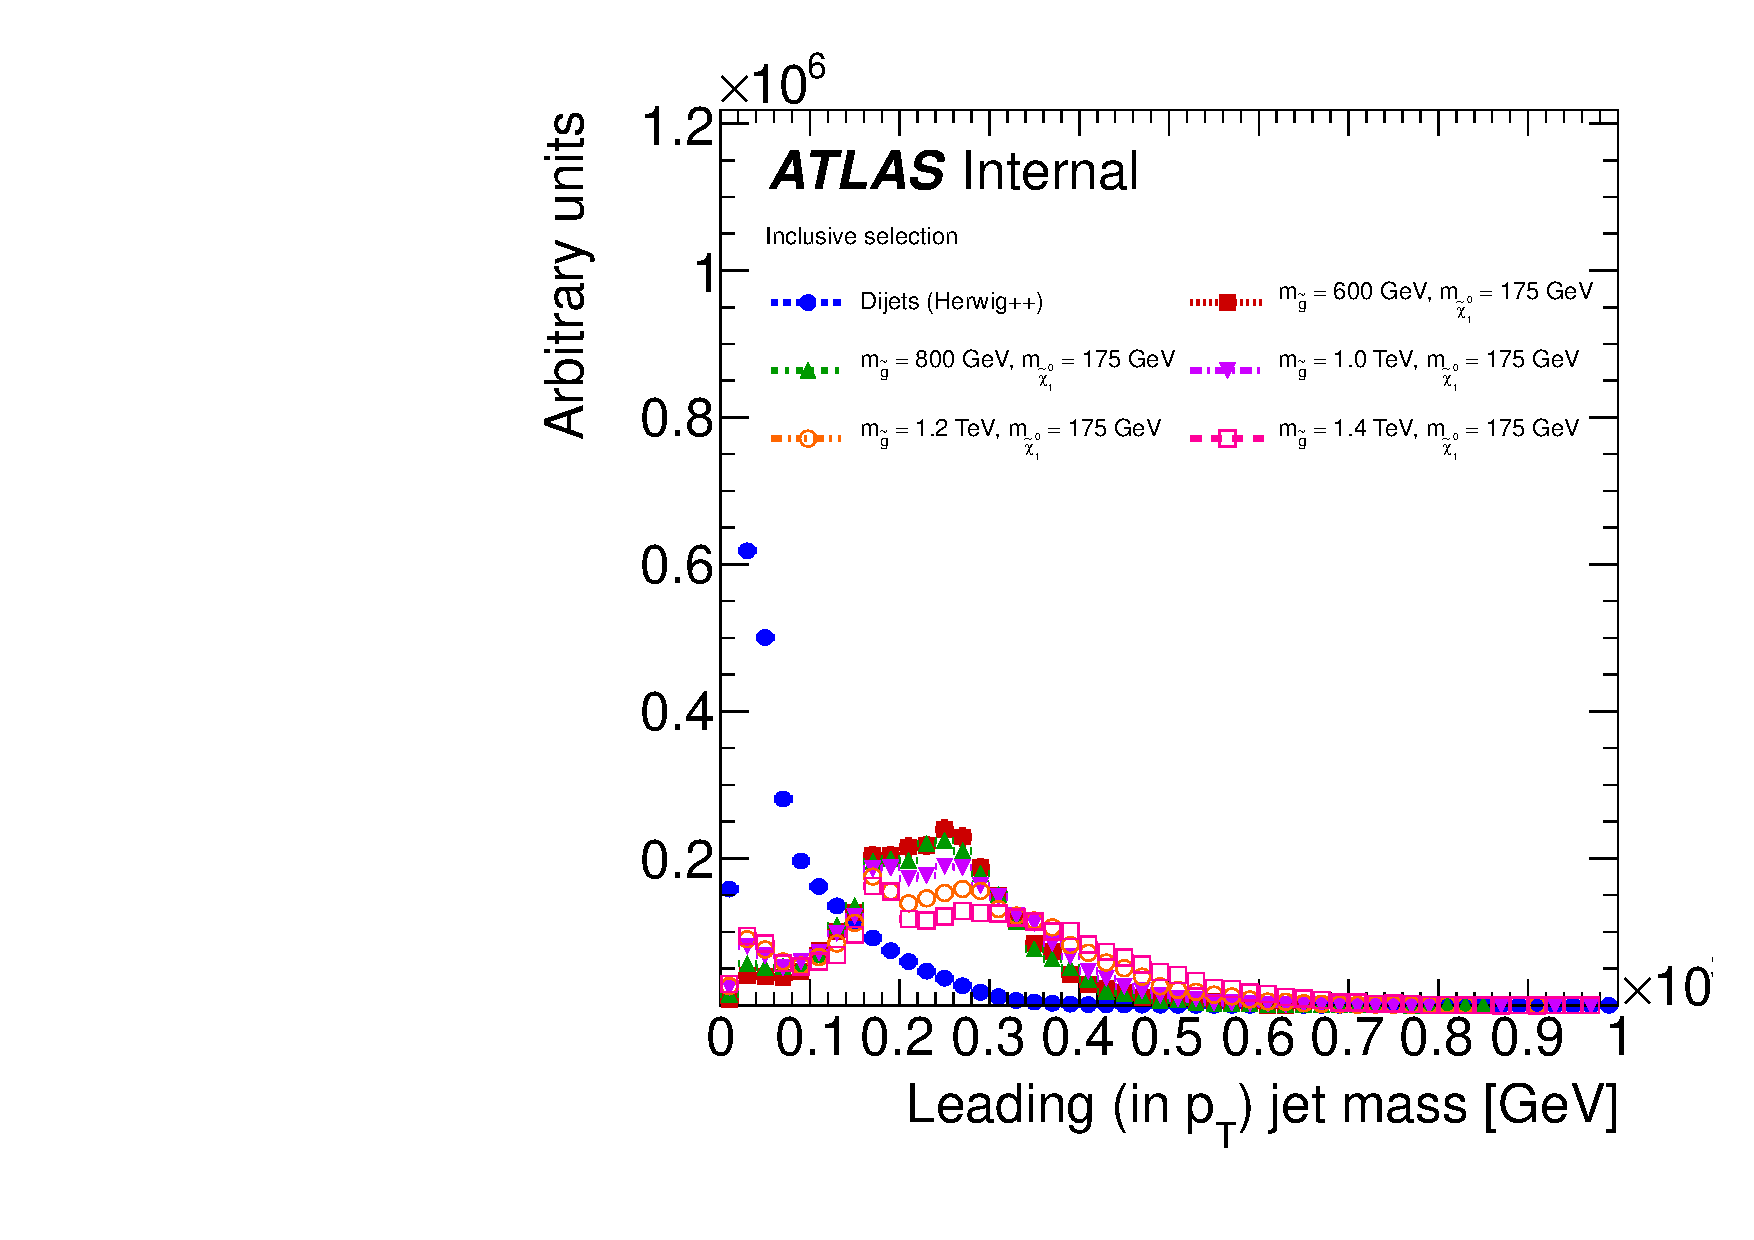
\includegraphics[width=0.45\columnwidth]{INT/Discrimination/overlay_jet_mass1_signalComparison_TopMass_Incl_j470_AntiKt10LCTopoTrimmedPtFrac5SmallR30_data12_v22.pdf}~
    \label{fig:search:search:optimization:signalcomp1:topmg}}

    
  \caption{Leading jet mass distributions for many different signal mass points, compared to the \texttt{Herwig++} dijet background. 
           }
           
  \label{fig:search:search:optimization:signalcomp1}
\end{figure}

%%------------------------------    

\begin{figure}[!ht]
  \centering
  
  \subfigure[High boost mass points.]{
    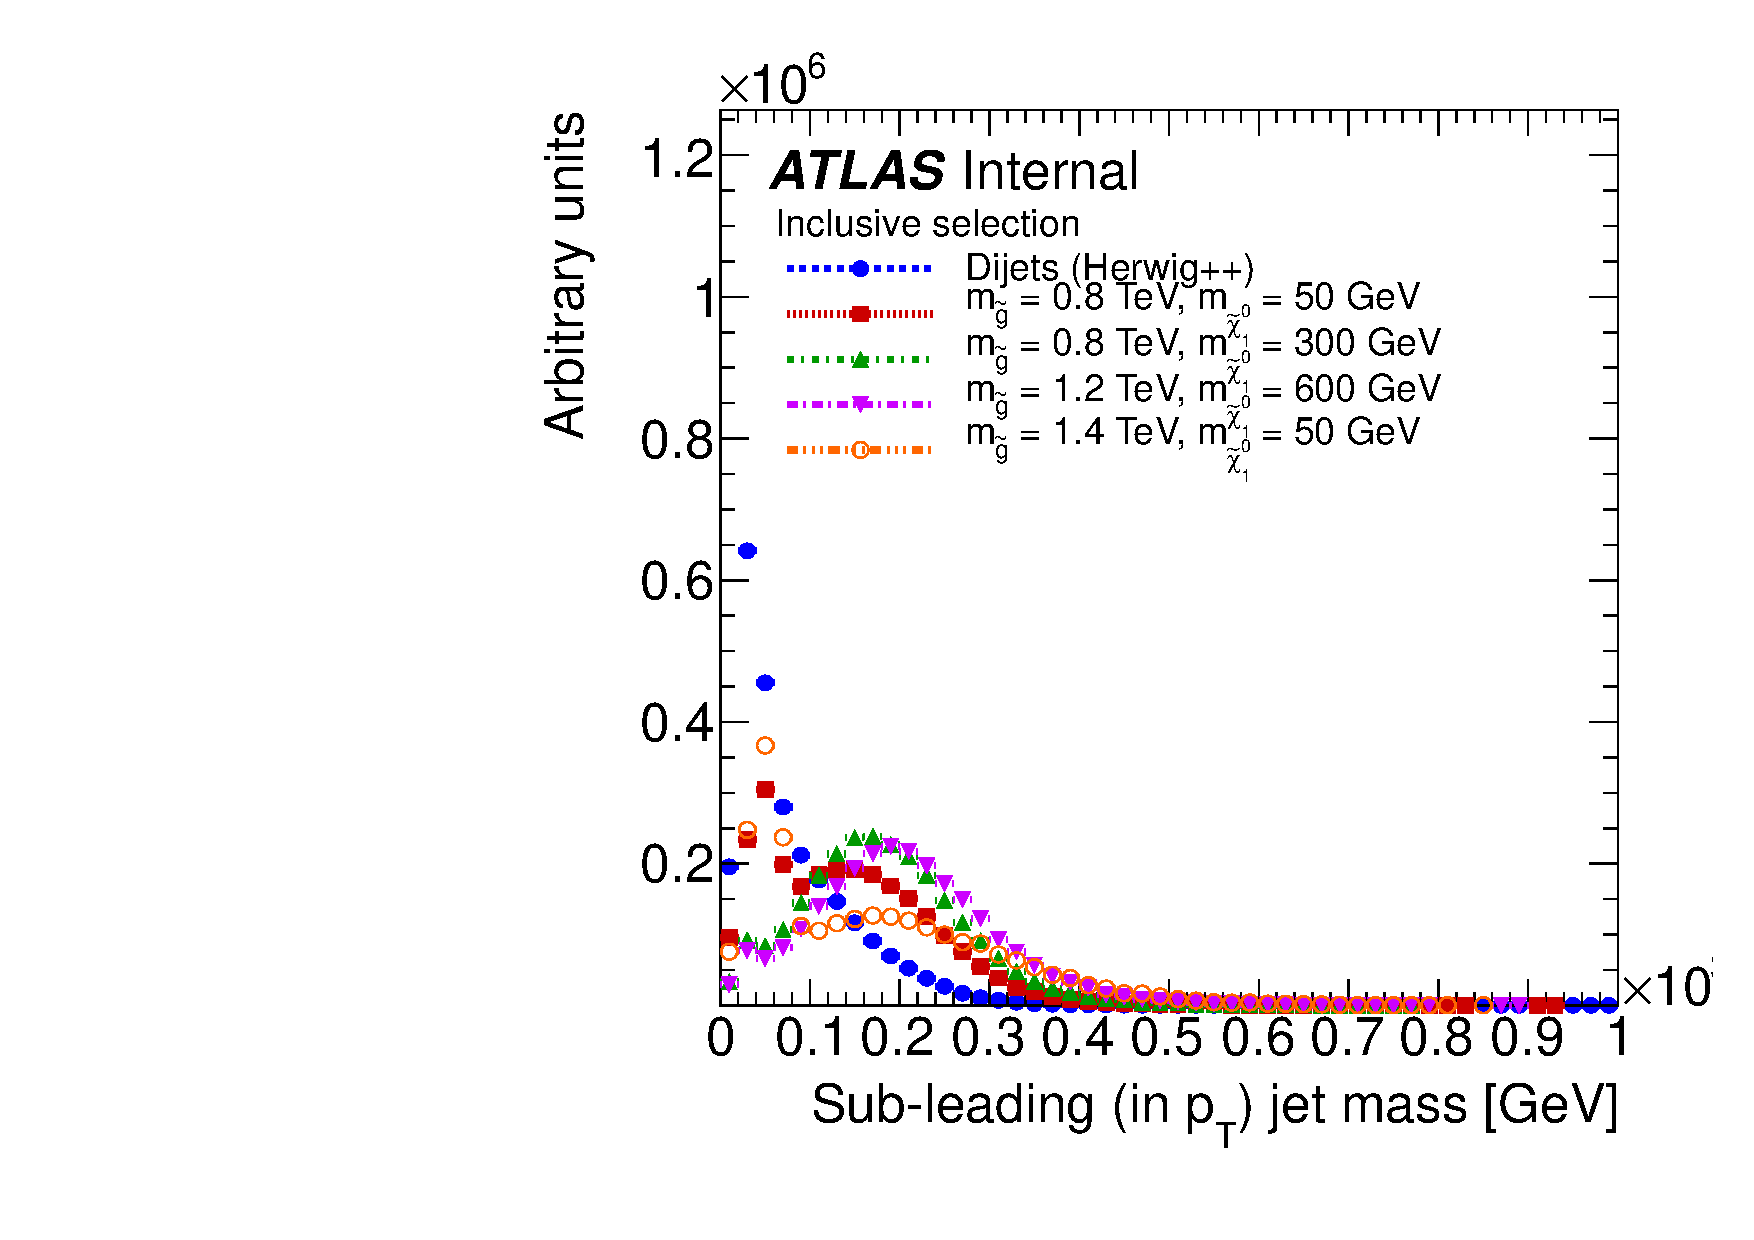
\includegraphics[width=0.45\columnwidth]{INT/Discrimination/overlay_jet_mass2_signalComparison_highBoost_Incl_j470_AntiKt10LCTopoTrimmedPtFrac5SmallR30_data12_v22.pdf}
    \label{fig:search:search:optimization:signalcomp2:highboost}}~
  \subfigure[High $\mgluino$ mass points]{
    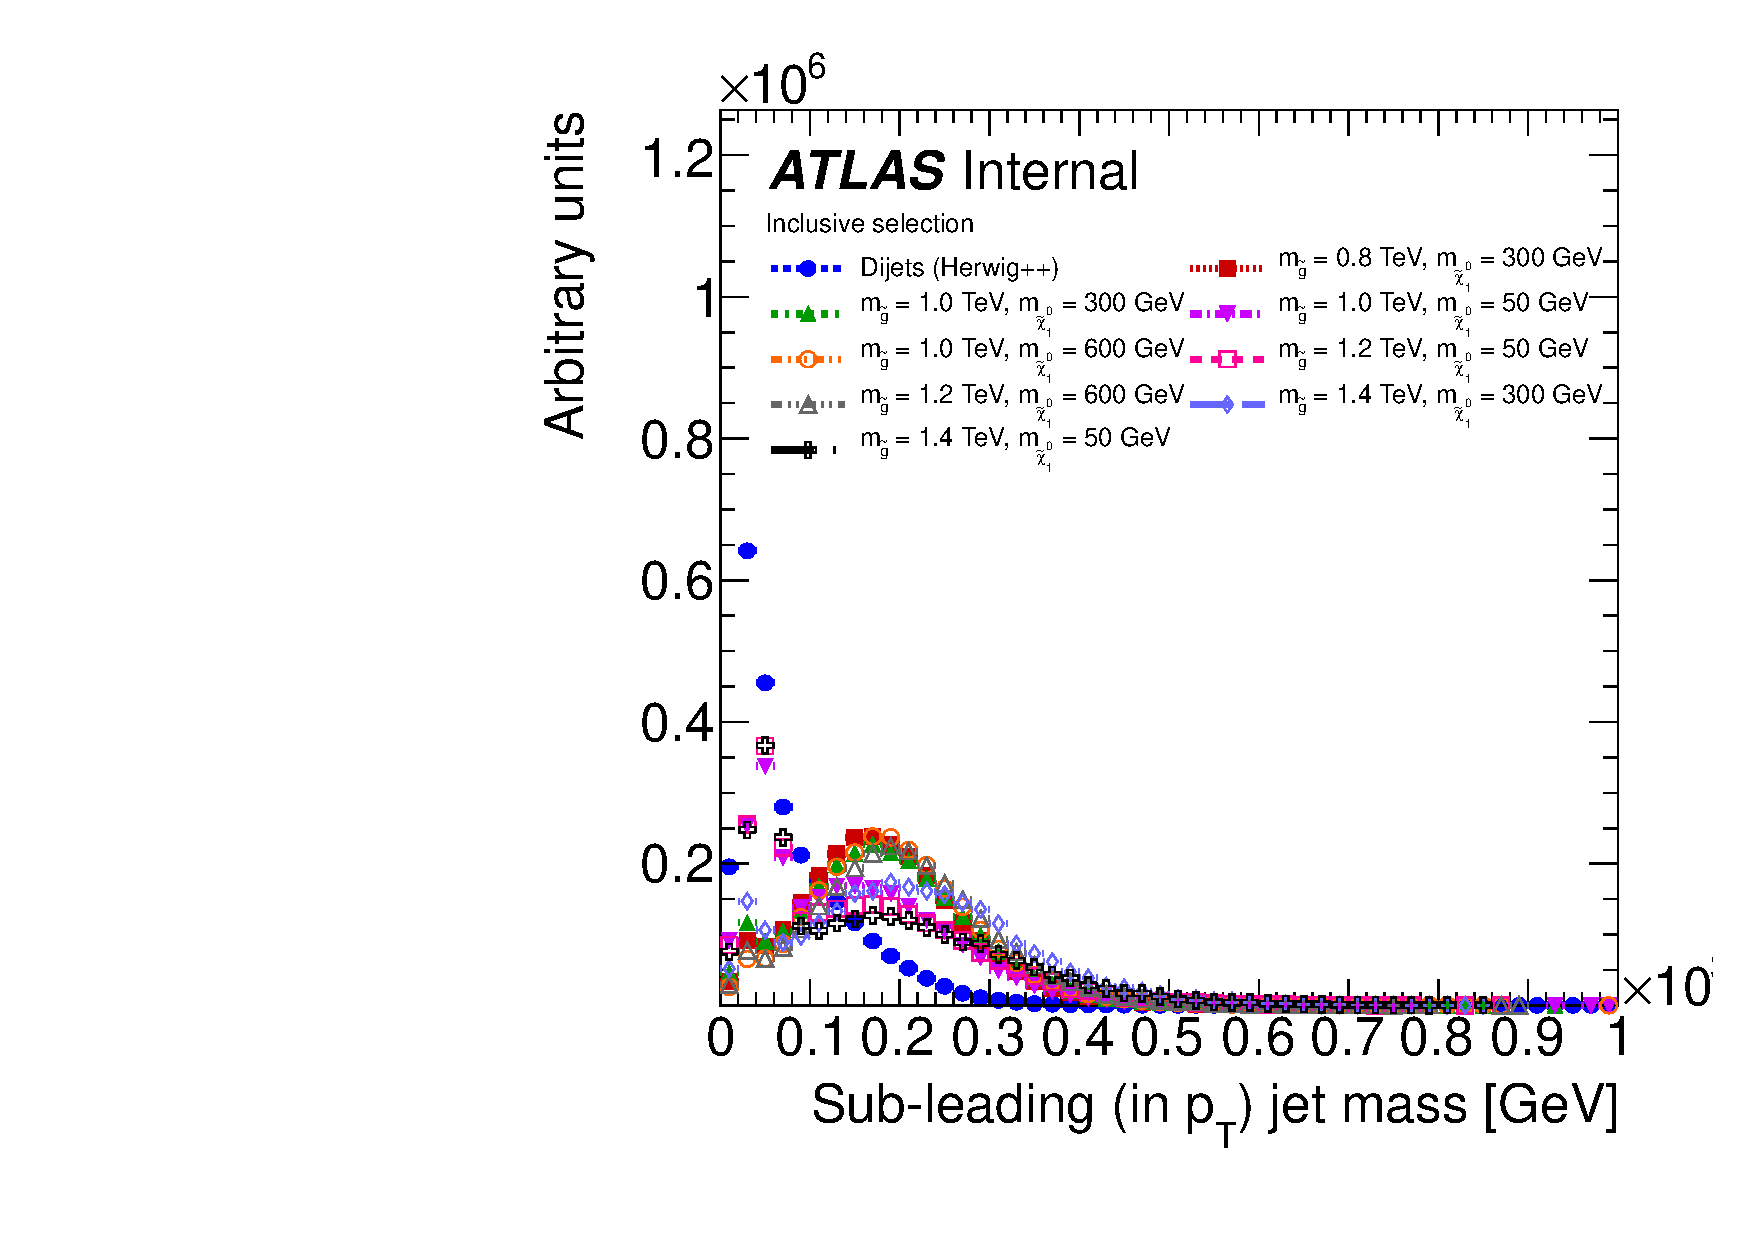
\includegraphics[width=0.45\columnwidth]{INT/Discrimination/overlay_jet_mass2_signalComparison_highGluinoM_Incl_j470_AntiKt10LCTopoTrimmedPtFrac5SmallR30_data12_v22.pdf}
    \label{fig:search:search:optimization:signalcomp2:highmg}}
  \subfigure[$\mgluino = 1$ TeV mass points]{
    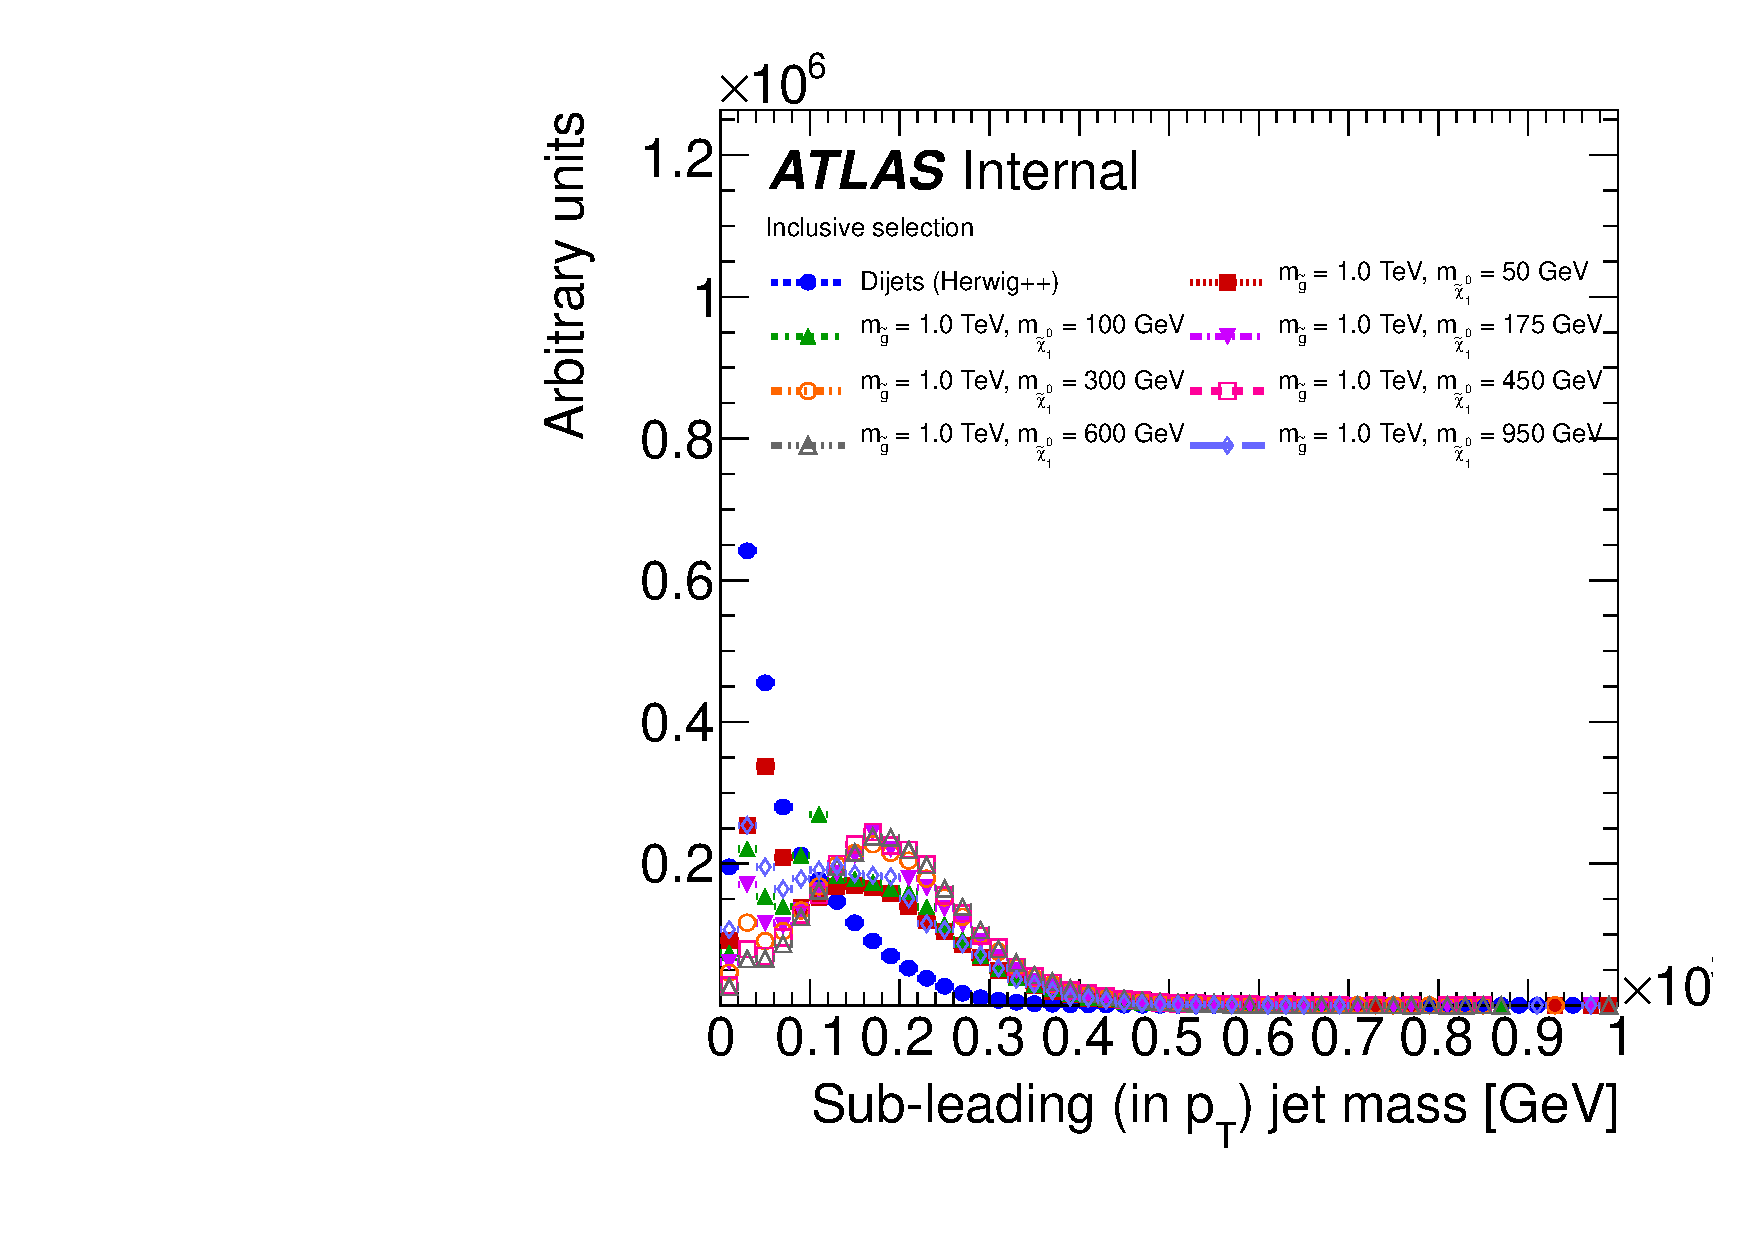
\includegraphics[width=0.45\columnwidth]{INT/Discrimination/overlay_jet_mass2_signalComparison_OneTeV_Incl_j470_AntiKt10LCTopoTrimmedPtFrac5SmallR30_data12_v22.pdf}~
    \label{fig:search:search:optimization:signalcomp2:tevmg}}
  \subfigure[$\sim$Top mass points]{
    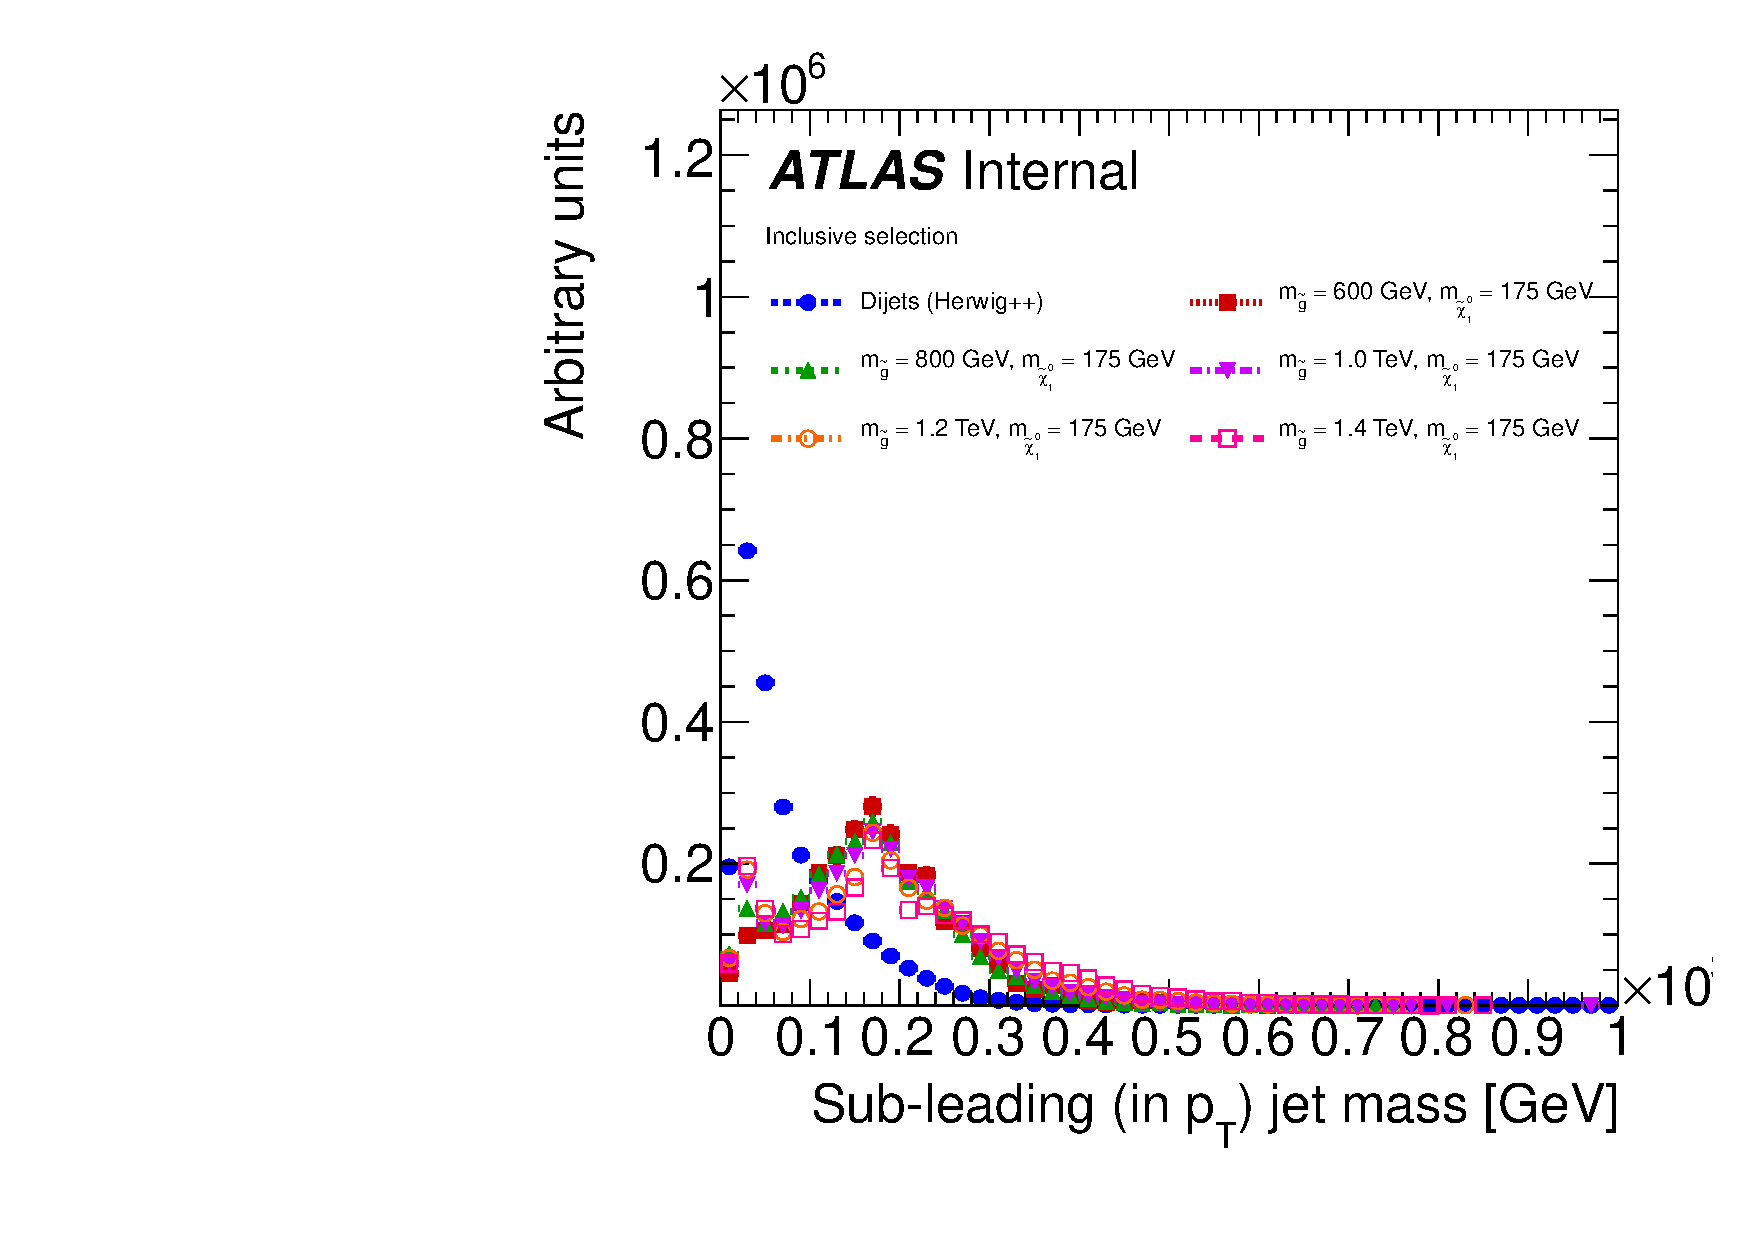
\includegraphics[width=0.45\columnwidth]{INT/Discrimination/overlay_jet_mass2_signalComparison_TopMass_Incl_j470_AntiKt10LCTopoTrimmedPtFrac5SmallR30_data12_v22.pdf}~
    \label{fig:search:search:optimization:signalcomp2:topmg}}

    
  \caption{Subleading jet mass distributions for many different signal mass points, compared to the \texttt{Herwig++} dijet background. 
           }
           
  \label{fig:search:search:optimization:signalcomp2}
\end{figure}

%%------------------------------    

Finally, while our main goal is to study the \gluino-\lsp model inclusively in flavor, it is interesting to consider whether we are particularly sensitive, for example, to \gluino decays mediated through $\tilde{t}$, or whether we are pick out mostly \lsp decays to $\tilde{t}$. In principle, top decays should slightly increase the quark multiplicity, as leptonic decays produce only one quark and hadronic decays produce three. While it is difficult to tell because of the limited statistics in the flavor-sliced samples, Figure~\ref{fig:search:search:optimization:flavor} shows the difference between situations in which the \gluino or \lsp decay to tops, compared to an inclusive sample. Both the \MJ and leading jet mass are approximately consistent over these comparisons, showing that the analysis selects flavor without large amounts of bias.


%%------------------------------
\begin{figure}[!ht]
  \centering

  \subfigure[Jet $M_{J,4}^{\Sigma}$]{
    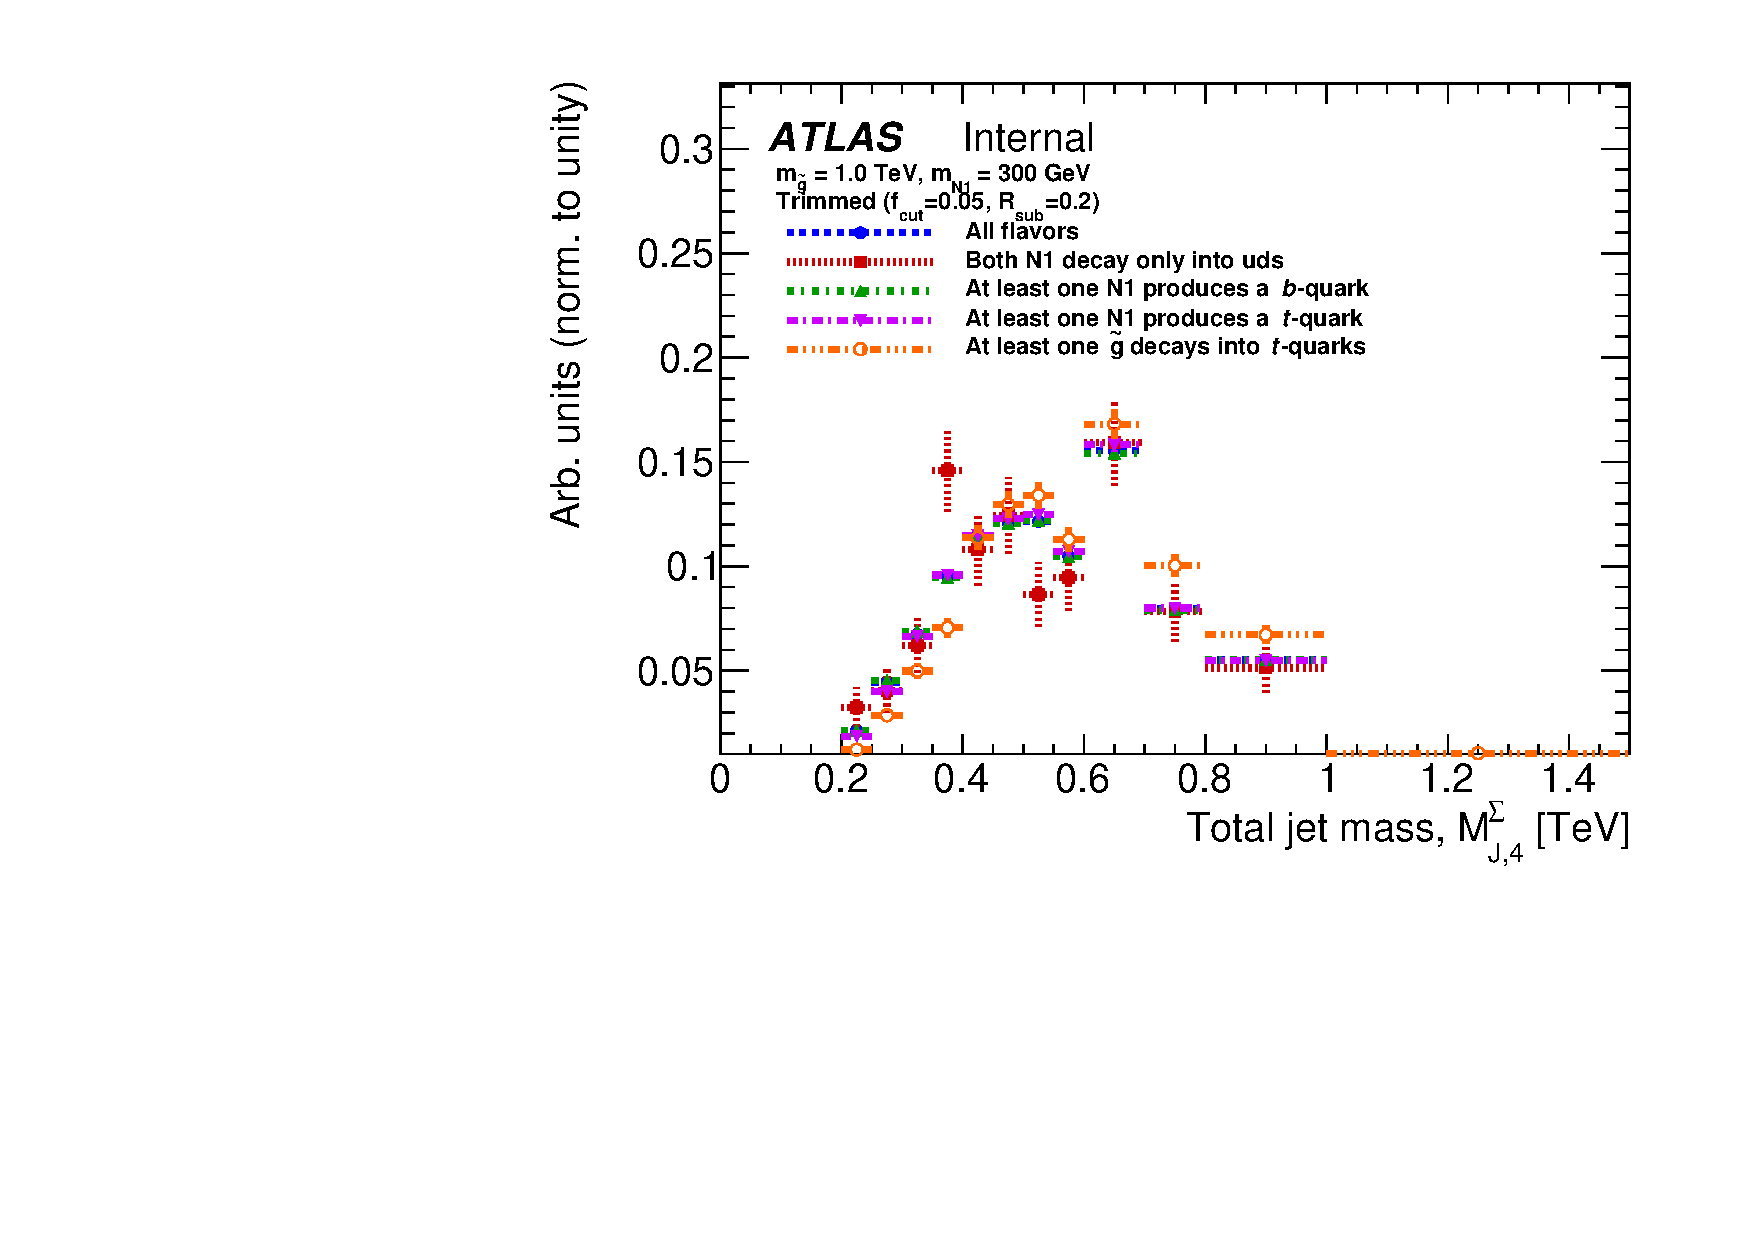
\includegraphics[width=0.48\textwidth]{INT/FlavorStudies/overlay_MJ4_jetComparison_all_AntiKt10LCTopoTrimmedPtFrac5SmallR30_Trimmed.pdf}
    \label{fig:search:search:optimization:flavor:mj4}}
  \subfigure[Jet $m_{j,1}$]{
    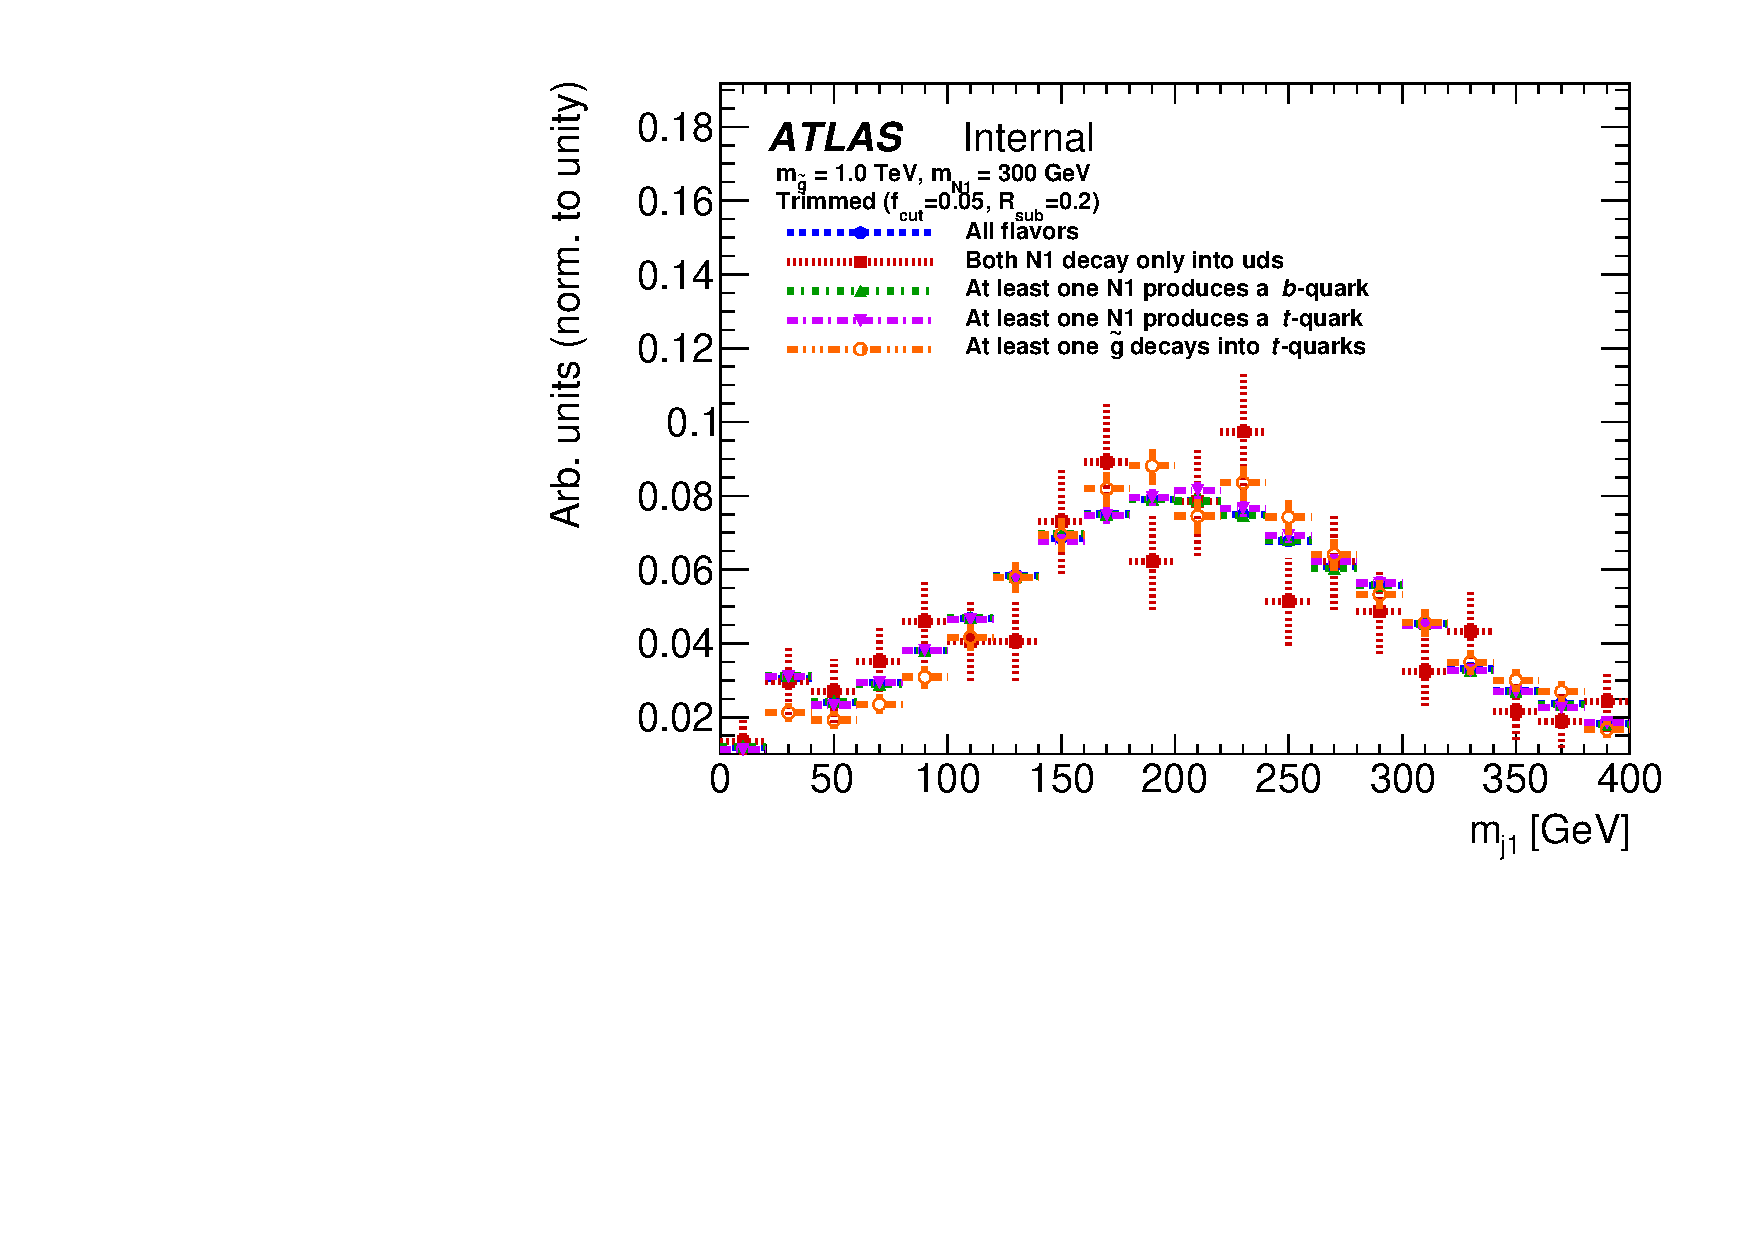
\includegraphics[width=0.48\textwidth]{INT/FlavorStudies/overlay_jet_mass1_jetComparison_all_AntiKt10LCTopoTrimmedPtFrac5SmallR30_Trimmed.pdf}
    \label{fig:search:search:optimization:flavor:m1}}
  
    \caption{Mass distributions for different truth particle final state flavors. The shape of the distributions was shown to be approximately independent of the final state.}
  \label{fig:search:search:optimization:flavor}
\end{figure}
%%------------------------------

\subsubsection{Two-Dimensional Optimization}

The second phase of optimization involves deciding on variable to be used in combination with \MJ. Additionally, as this second variable is meant to determine the creation of signal and control regions, it should not be strongly correlated with \MJ: large correlations could bias the information determined in a control region, such that it would not be directly applicable to a signal region anymore.

The easiest way to see the differences between pairs of variables is to construct two dimensional likelihoods, defining:
%
\begin{equation}
L = \frac{S}{S+B}
\end{equation}
%
where $S$ and $B$ are two-dimensional histograms in the two variables of interest, separately for signal and background. A useful pair of variables will have a high $L$ in a corner of this space: this would indicate that both variables are useful, and that they provide complementary information. Highly correlated variables appear as a line: this indicates that the power of one variable is strongly associated to a second, and that a cut on only one of them would be sufficient. 

Figure~\ref{fig:search:search:optimization:2D:NCA} and \ref{fig:search:search:optimization:2D:NKT}, for example, show the likelihoods formed with the subjet counting variables. While $N_{CA}$ and $N_{kT}$ are useful on their own, they provide little information on top of $\MJ$: a horizontal cut in this plane would provide just as much power as a diagonal (or curved) cut. The correlation levels in the background between \MJ and these variables is over $60\%$, indicating that indeed little additional information is contained. $T_{32}$ and $T_{21}$ are also similarly correlated to \MJ, and therefore are also not particularly useful.


%%%%%%%%%%%%%%%%

\begin{figure}
\centering
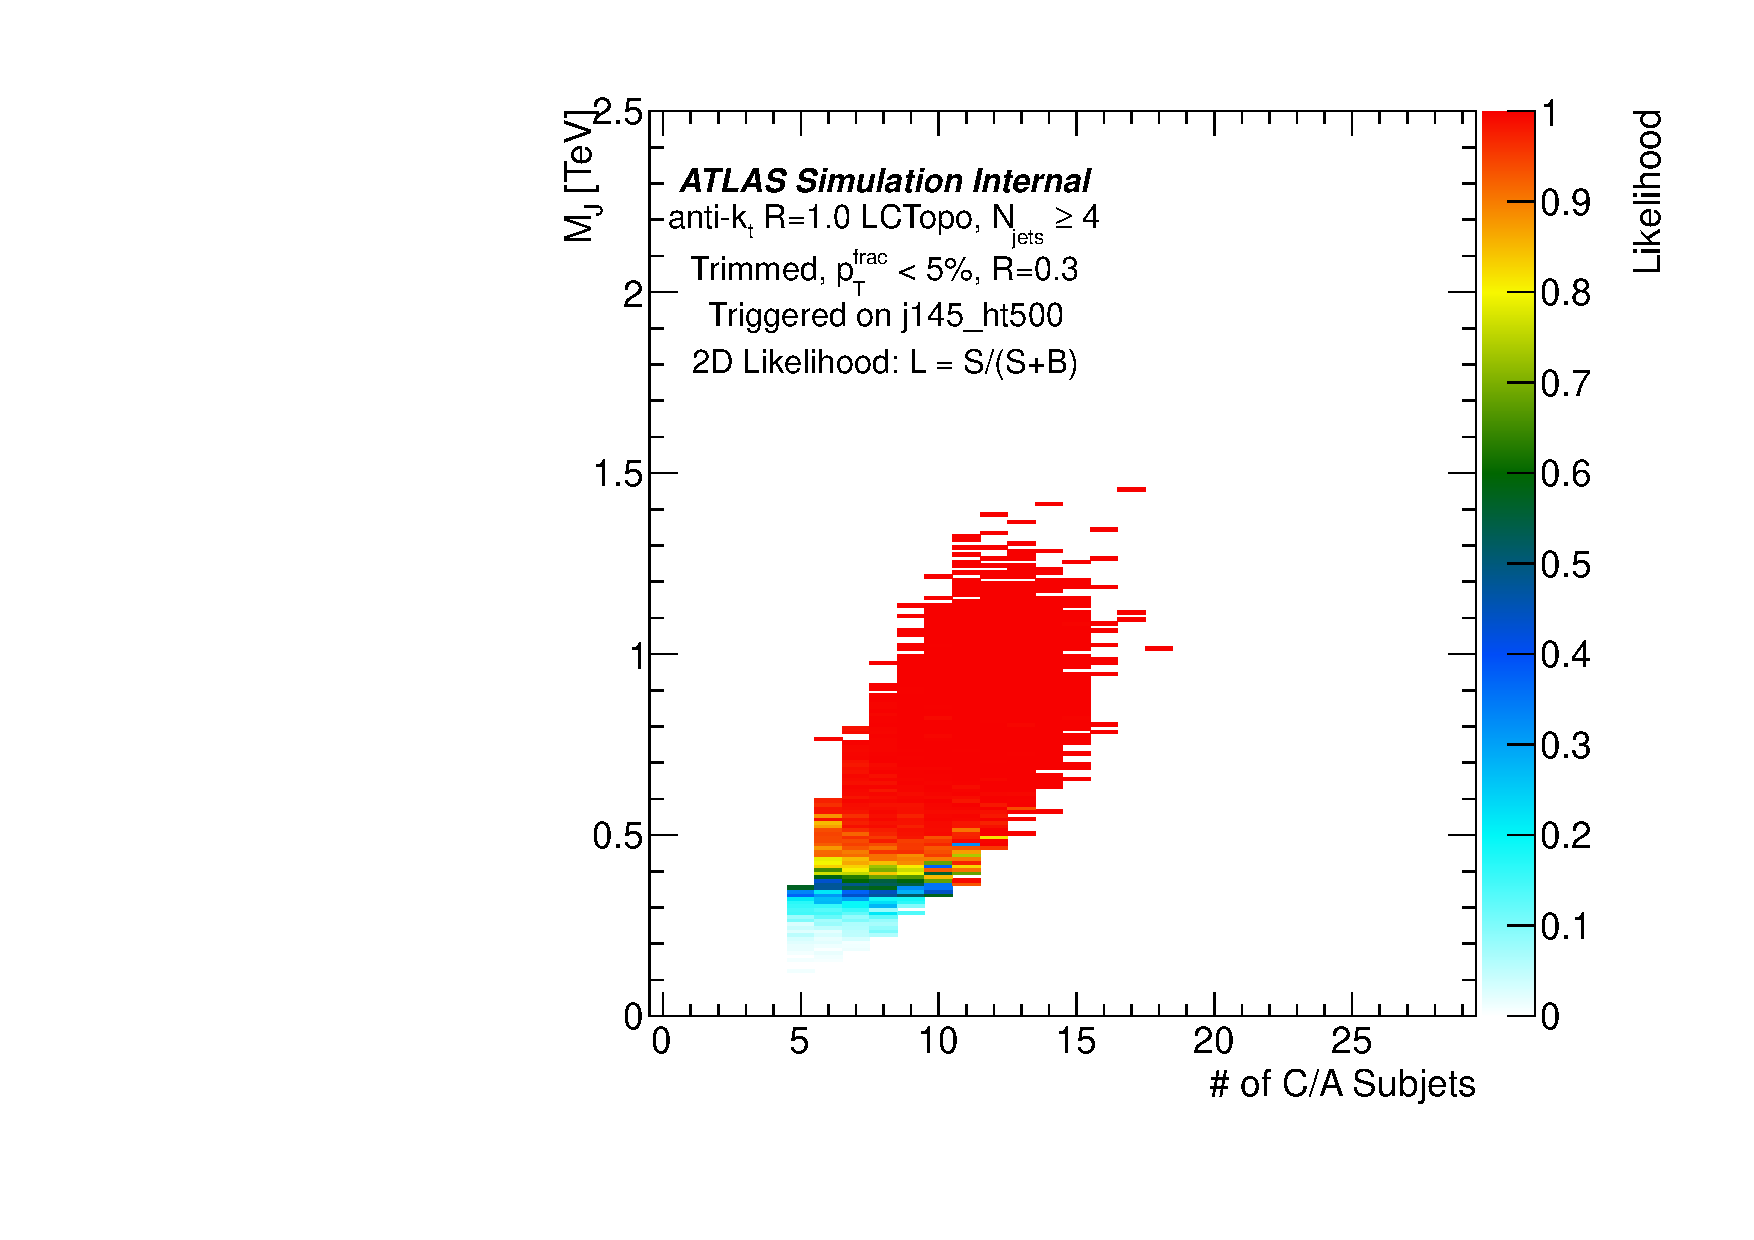
\includegraphics[width=0.5\textwidth]{INT/AntiKt10LCTopoTrimmedPtFrac5SmallR30_j145_ht500_NjetIncl_NFatJetMin4_MJ4_vs_NCASub4_SigPoint1_L_RPVGluino.pdf}
\label{fig:search:search:optimization:2D:NCA}
\caption{A likelihood for discrimination between a high $m_{\gluino}$ point and a \herwigpp di-jet background, using \MJ and $N_{CA}$ as inputs.}
\end{figure}

%%%%%%%%%%%%%%%%  


%%%%%%%%%%%%%%%%

\begin{figure}
\centering
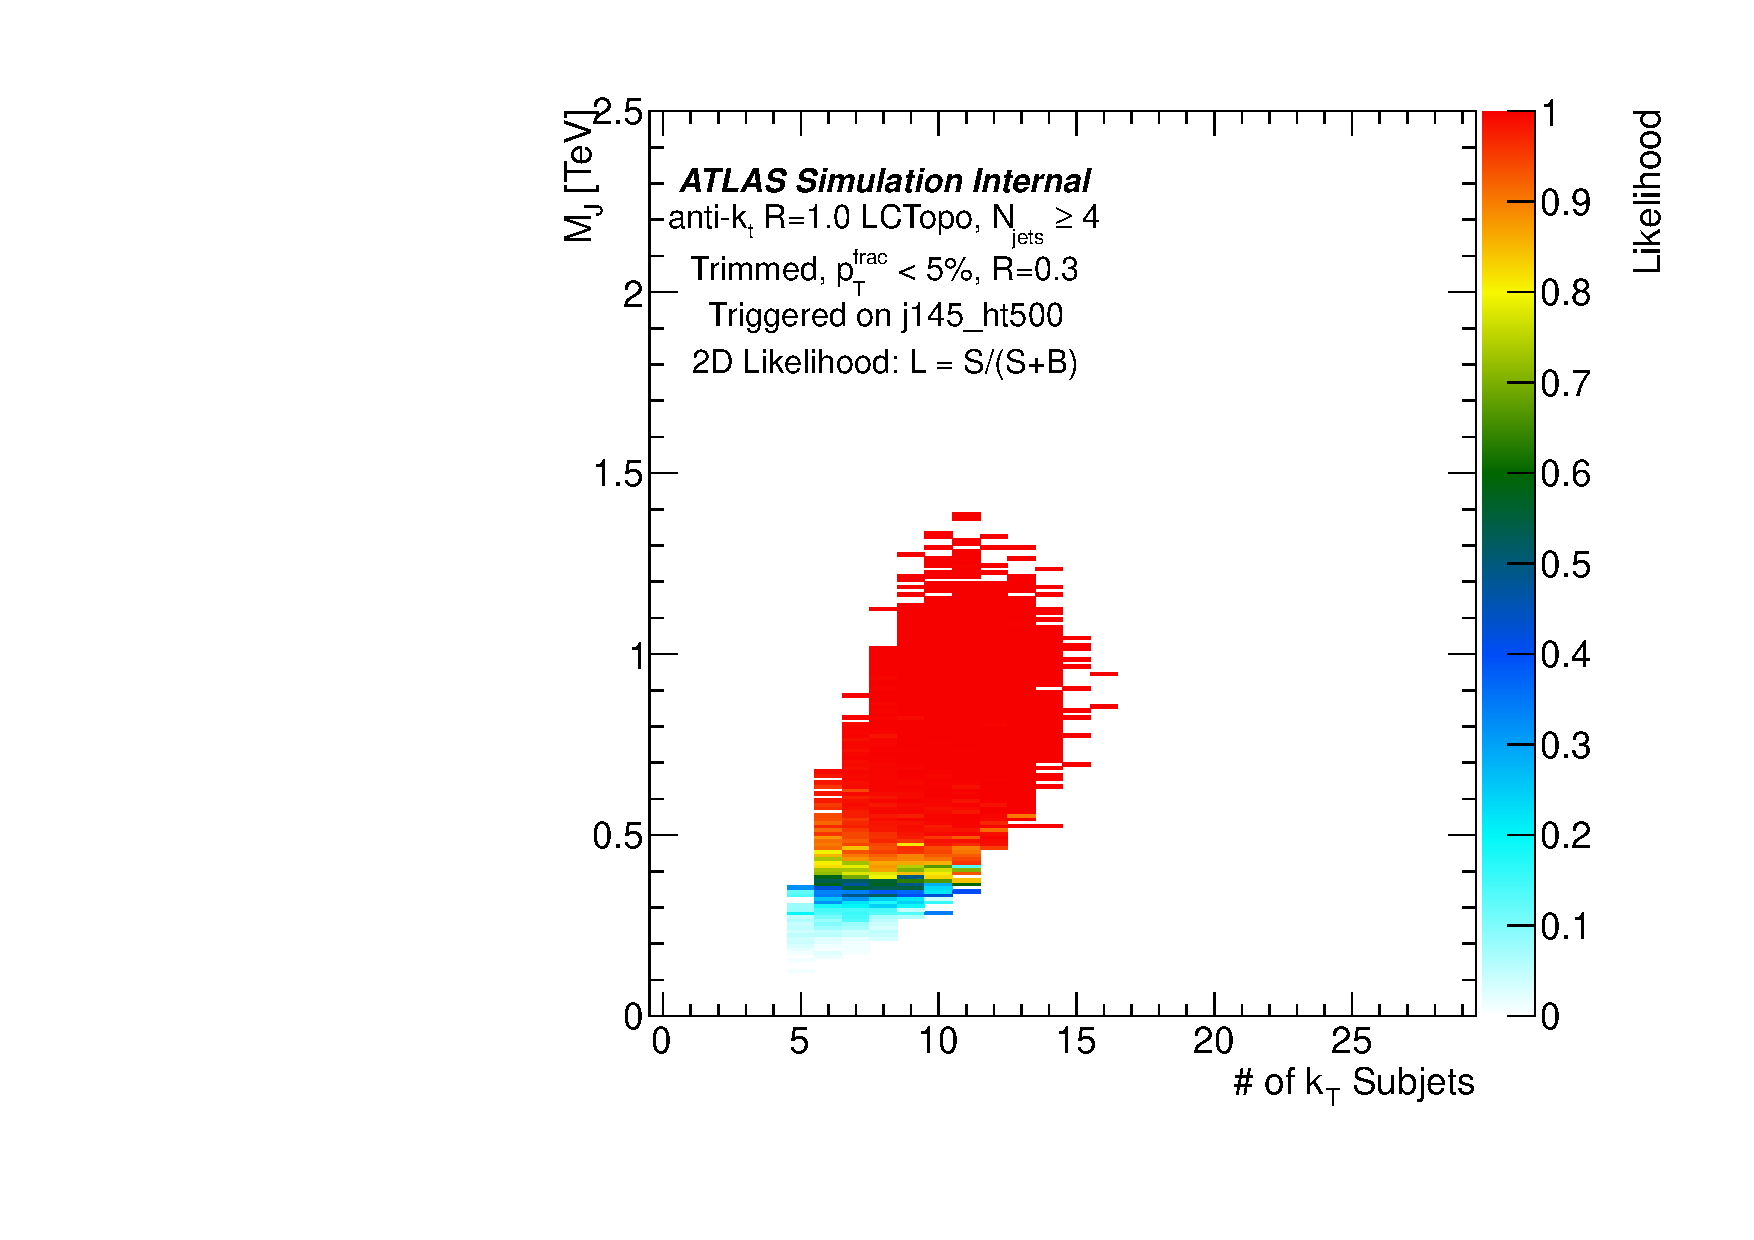
\includegraphics[width=0.5\textwidth]{INT/AntiKt10LCTopoTrimmedPtFrac5SmallR30_j145_ht500_NjetIncl_NFatJetMin4_MJ4_vs_NKTSub4_SigPoint1_L_RPVGluino.pdf}
\label{fig:search:search:optimization:2D:NKT}
\caption{A likelihood for discrimination between a high $m_{\gluino}$ point and a \herwigpp di-jet background, using \MJ and $N_{kt}$ as inputs.}
\end{figure}

%%%%%%%%%%%%%%%% 


Other variables have less correlation, and therefore potentially improved utility. Figure~\ref{fig:search:search:optimization:2D:PT31}, for example, shows the likelihood constructed with $\pt^3/\pt^1$: a diagonal cut, incorporating the discriminating power of both variables, would be clearly helpful. In this case, the correlation in the background between the two variables is at $20\%$: still substantial, but significantly reduced compared to the substructure based variables. This is reasonable, as all substructure variables are correlated to some extent: mass arises from the presence of wild angle radiation, which also causes extra subjets or lower talues of $\tau_{32}$, etc. Kinematic information like \pt is slightly correlated with masses as well, but less when looking at a ratio of \pt's, and looking at only some of the jets (instead of \Ht, which looks at the \pt of all them like much like \MJ).

%%%%%%%%%%%%%%%%

\begin{figure}
\centering
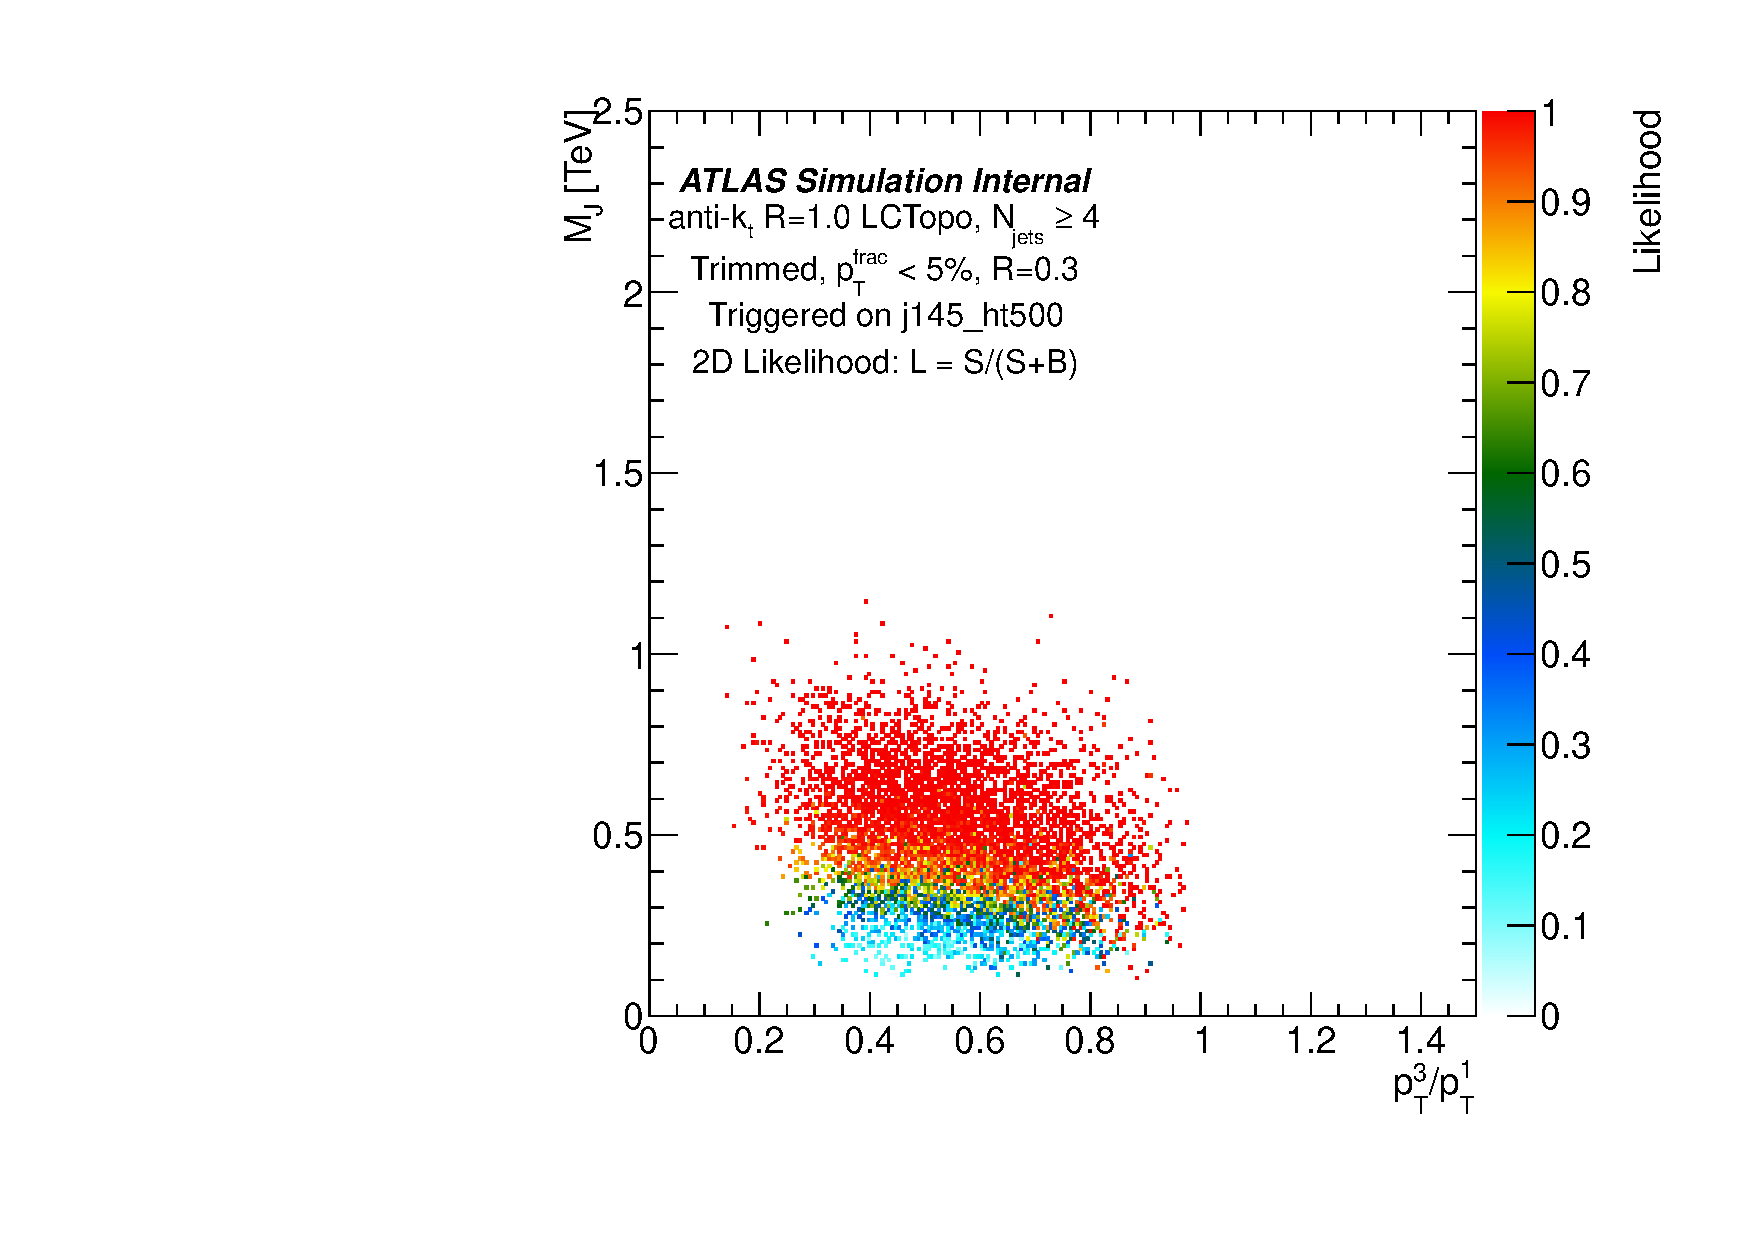
\includegraphics[width=0.5\textwidth]{INT/AntiKt10LCTopoTrimmedPtFrac5SmallR30_j145_ht500_NjetIncl_NFatJetMin4_MJ4_vs_PT31_SigPoint3_L_RPVGluino.pdf}
\label{fig:search:search:optimization:2D:PT31}
\caption{A likelihood for discrimination between a high $m_{\gluino}$ point and a \herwigpp di-jet background, using \MJ and $\pt^3/\pt^1$ as inputs.}
\end{figure}

%%%%%%%%%%%%%%%%  

Finally, Figure~\ref{fig:search:search:optimization:2D:DETA} shows the likelihood constructed with \Deta. Once again, the discrimination is improved by a diagonal cut, and even better, the correlation is significantly lower in these variables, at $<10\%$. Figure~\ref{fig:search:search:optimization:2D:DETAraw} shows the distribution in the \herwigpp di-jet sample: this evident very low level of correlation between the variables makes \Deta ideal to define signal and control regions, as will be discussed in Section~\ref{chapter:search:search:regions}. For this reason, the two variables used to define the analysis were chosen to be \MJ and \Deta.

%%%%%%%%%%%%%%%%

\begin{figure}
\centering
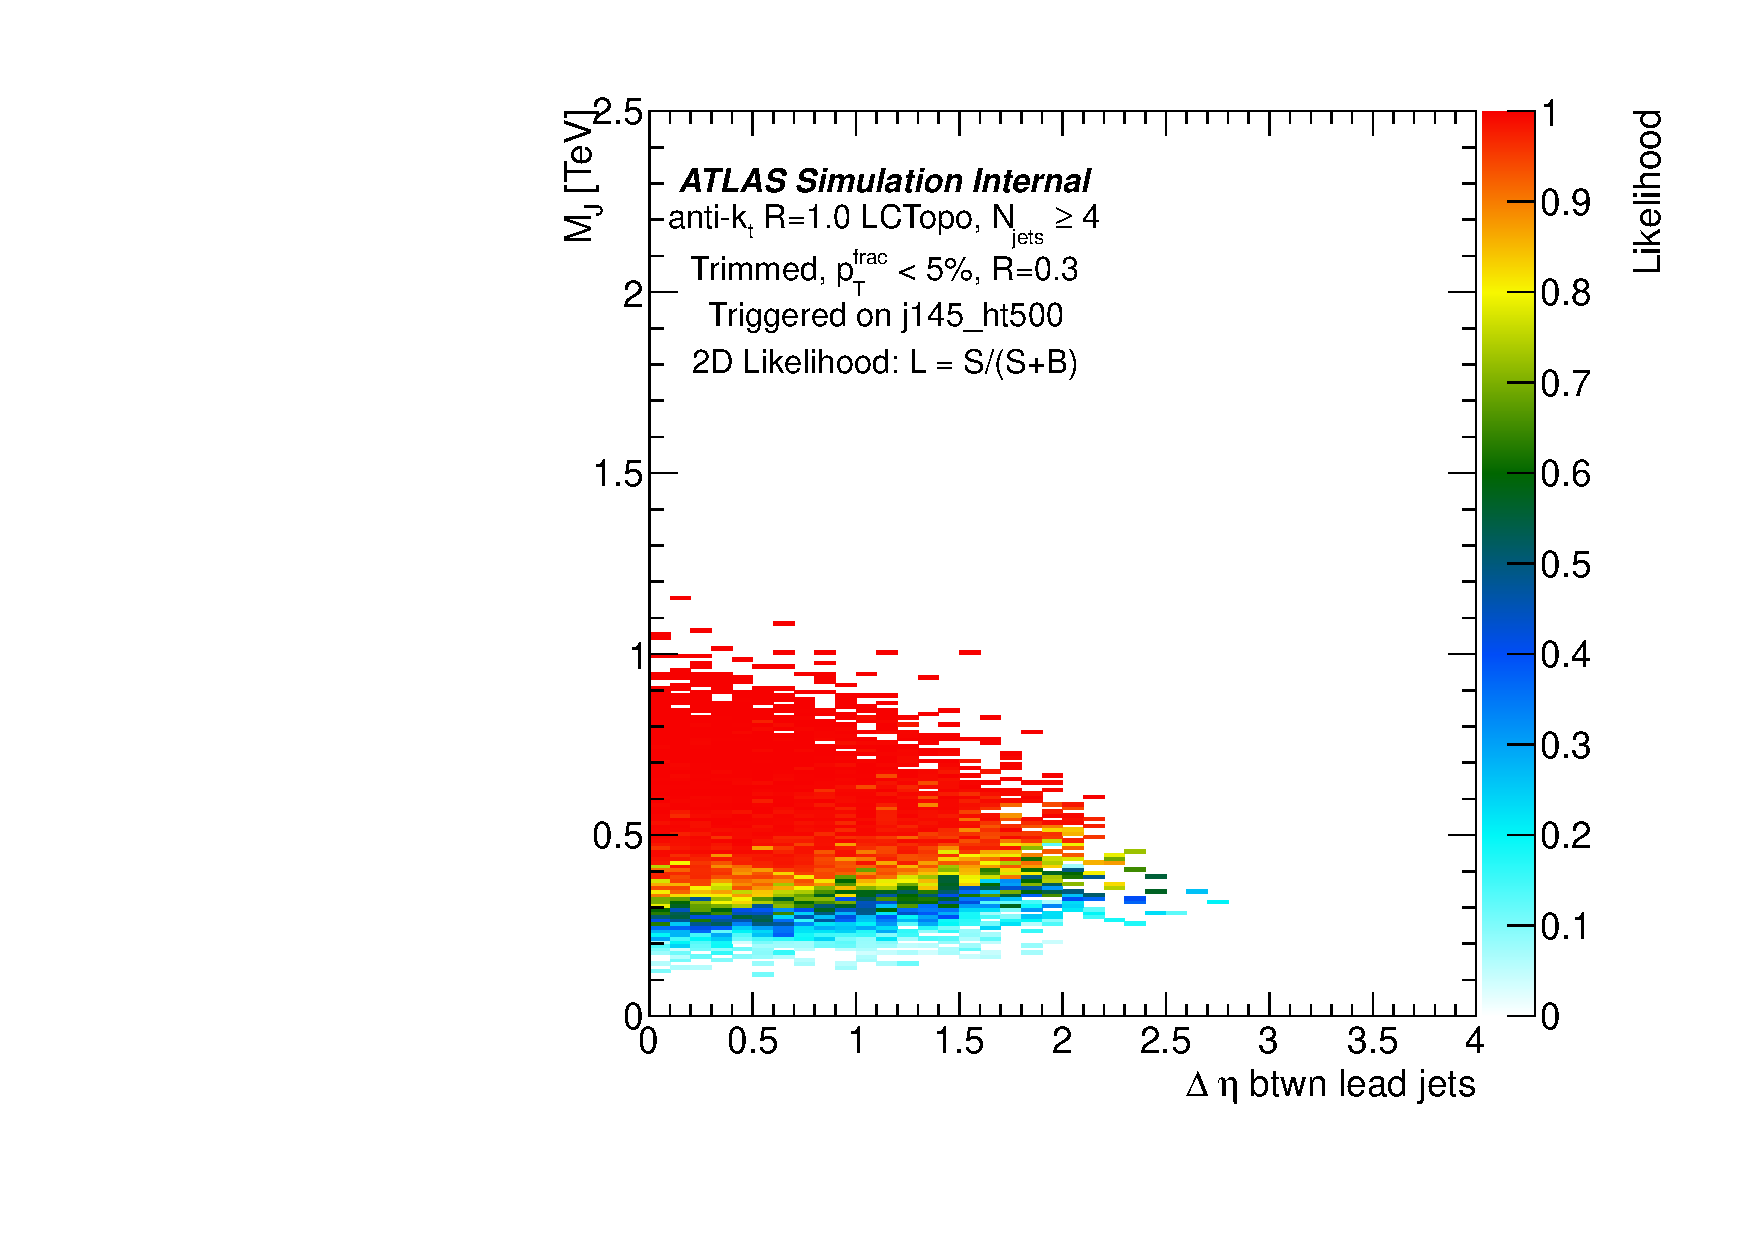
\includegraphics[width=0.5\textwidth]{INT/AntiKt10LCTopoTrimmedPtFrac5SmallR30_j145_ht500_NjetIncl_NFatJetMin4_MJ4_vs_DEta_SigPoint5_L_RPVGluino.pdf}
\label{fig:search:search:optimization:2D:DETA}
\caption{A likelihood for discrimination between a high $m_{\gluino}$ point and a \herwigpp di-jet background, using \MJ and $\Delta \eta$ as inputs.}
\end{figure}

%%%%%%%%%%%%%%%% 

%%%%%%%%%%%%%%%%

\begin{figure}
\centering
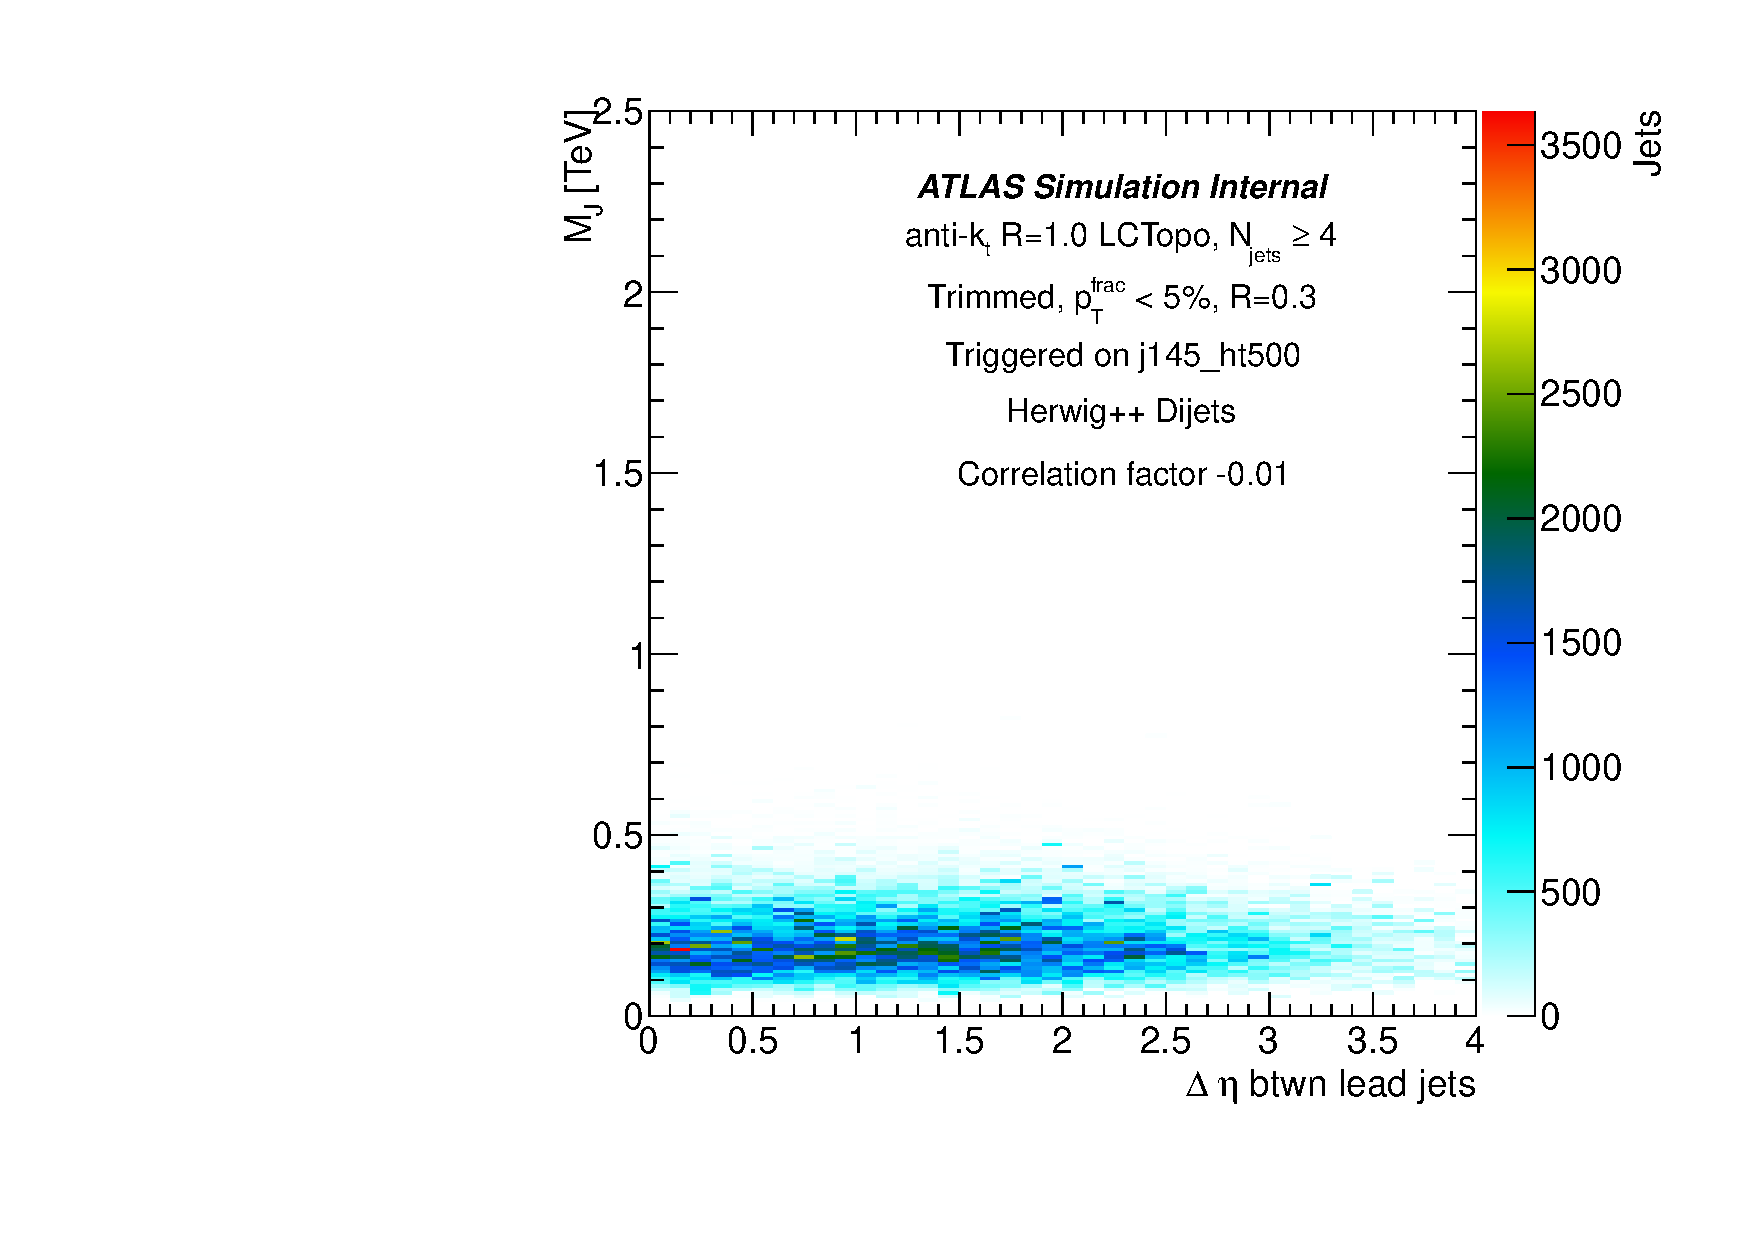
\includegraphics[width=0.5\textwidth]{INT/AntiKt10LCTopoTrimmedPtFrac5SmallR30_j145_ht500_NjetIncl_NFatJetMin4_MJ4_vs_DEta_SigPoint_RPVGluino.pdf}
\label{fig:search:search:optimization:2D:DETAraw}
\caption{A likelihood for discrimination between a high $m_{\gluino}$ point and a \herwigpp di-jet background, using \MJ and $\Delta \eta$ as inputs.}
\end{figure}

%%%%%%%%%%%%%%%% 


Note also that other combinations without \MJ were also considered: \Ht and $T_{32}$, for example, are subsantially less correlated because \Ht does not use substructure information. These pairings were all less effective than \MJ and \Deta combination. Additionally, pre-selection cuts on $T_{32}$ and $T_{21}$ were attempted, in combination with the \MJ and \Deta variables: adding the additional discrimination from the n-subjettiness variables did not significantly increase the discrimination.


\subsection{Event and Trigger Selections}

To perform the analysis in data, only events which pass a general quality selection and particular trigger configuration are used. The quality selection is rather generic to many ATLAS analyses:
%
\begin{enumerate}
\item Events are required to have not occurred during periods with limited detector operations.
\item Events are required to contain a primary vertex consistent with the LHC beamspot, reconstructed from at least 2 tracks with transverse momenta $\pt^{\mathrm{track}} > 400$~MeV
\item Jets reconstructed with the anti-kt algorithm using a size parameter of $R = 0.4$ and a measured $\pt^{\mathrm{jet}}$ > 25 GeV are required to satisfy the “looser” requirements, which are targetted at reducing background from photons and electrons (by requiring the EM fraction to be at least 5\%), as well as poorly functioning regions of the detector (by requiring that no jet be allowed to have more than 99\% of its energy in one layer)~\cite{jetquality}. Furthermore, jets with a majority of their energy in the HEC are required to have no problematic noise characteristics, and no more than 60 GeV of negative energy (both indications of read-out problems); jets enclosed in the ECal are required to have good pulse shapes in all layers. If any jet with $\pt^{\mathrm{jet}} > 25$~GeV is found to fail any of these criteria, the event is rejected.
\end{enumerate} 
%

A three-stage trigger system is used to select interesting events for the analysis. The Level-1 trigger... \editnote{Need to add L1 and L2 details!}


The high-\pt trigger at the event filter, \texttt{EF\_j360\_a10tcem}, has an online cut of $360$~GeV on the leading jet \pt, constructed using the \antikt $R=1.0$ algorithm from online EM-scale topo-clusters. Fluctuations due to jet energy resolution and differences between online and offline reconstruction (for example, the online jet has no trimming applied, and the clusters are only EM-scale instead of locally calibrated) mean that a jet with a given offline \pt may or may not have actually fired the trigger. As the modeling of the trigger in the simulation is somewhat unrelaible, we require the offline jet \pt to be fully efficient: i.e., that the \pt is so high that the trigger is guaranteed to have fired.

To measure the efficiency of the \texttt{j360} trigger, its measurements are compared to a \textit{reference} trigger. A reference trigger has a lower \pt threshold, but is pre-scaled to avoid taking data at too high a rate. A higher \pt threshold trigger is considered fully efficient if it fired on every event on which the lower \pt treshold trigger fired. The ratio of their efficiencies is called the \textit{turn-on} curve. In order to make the trigger fully efficient an offline \pt cut on the trimmed jet pT at $500$~GeV was used, as motivated by Figure~\ref{fig:search:search:trig:pt1}. 

%% pT1 and cum eff
\begin{figure}[!ht]
  \centering
  \subfigure[Leading $\ptjet$]{
    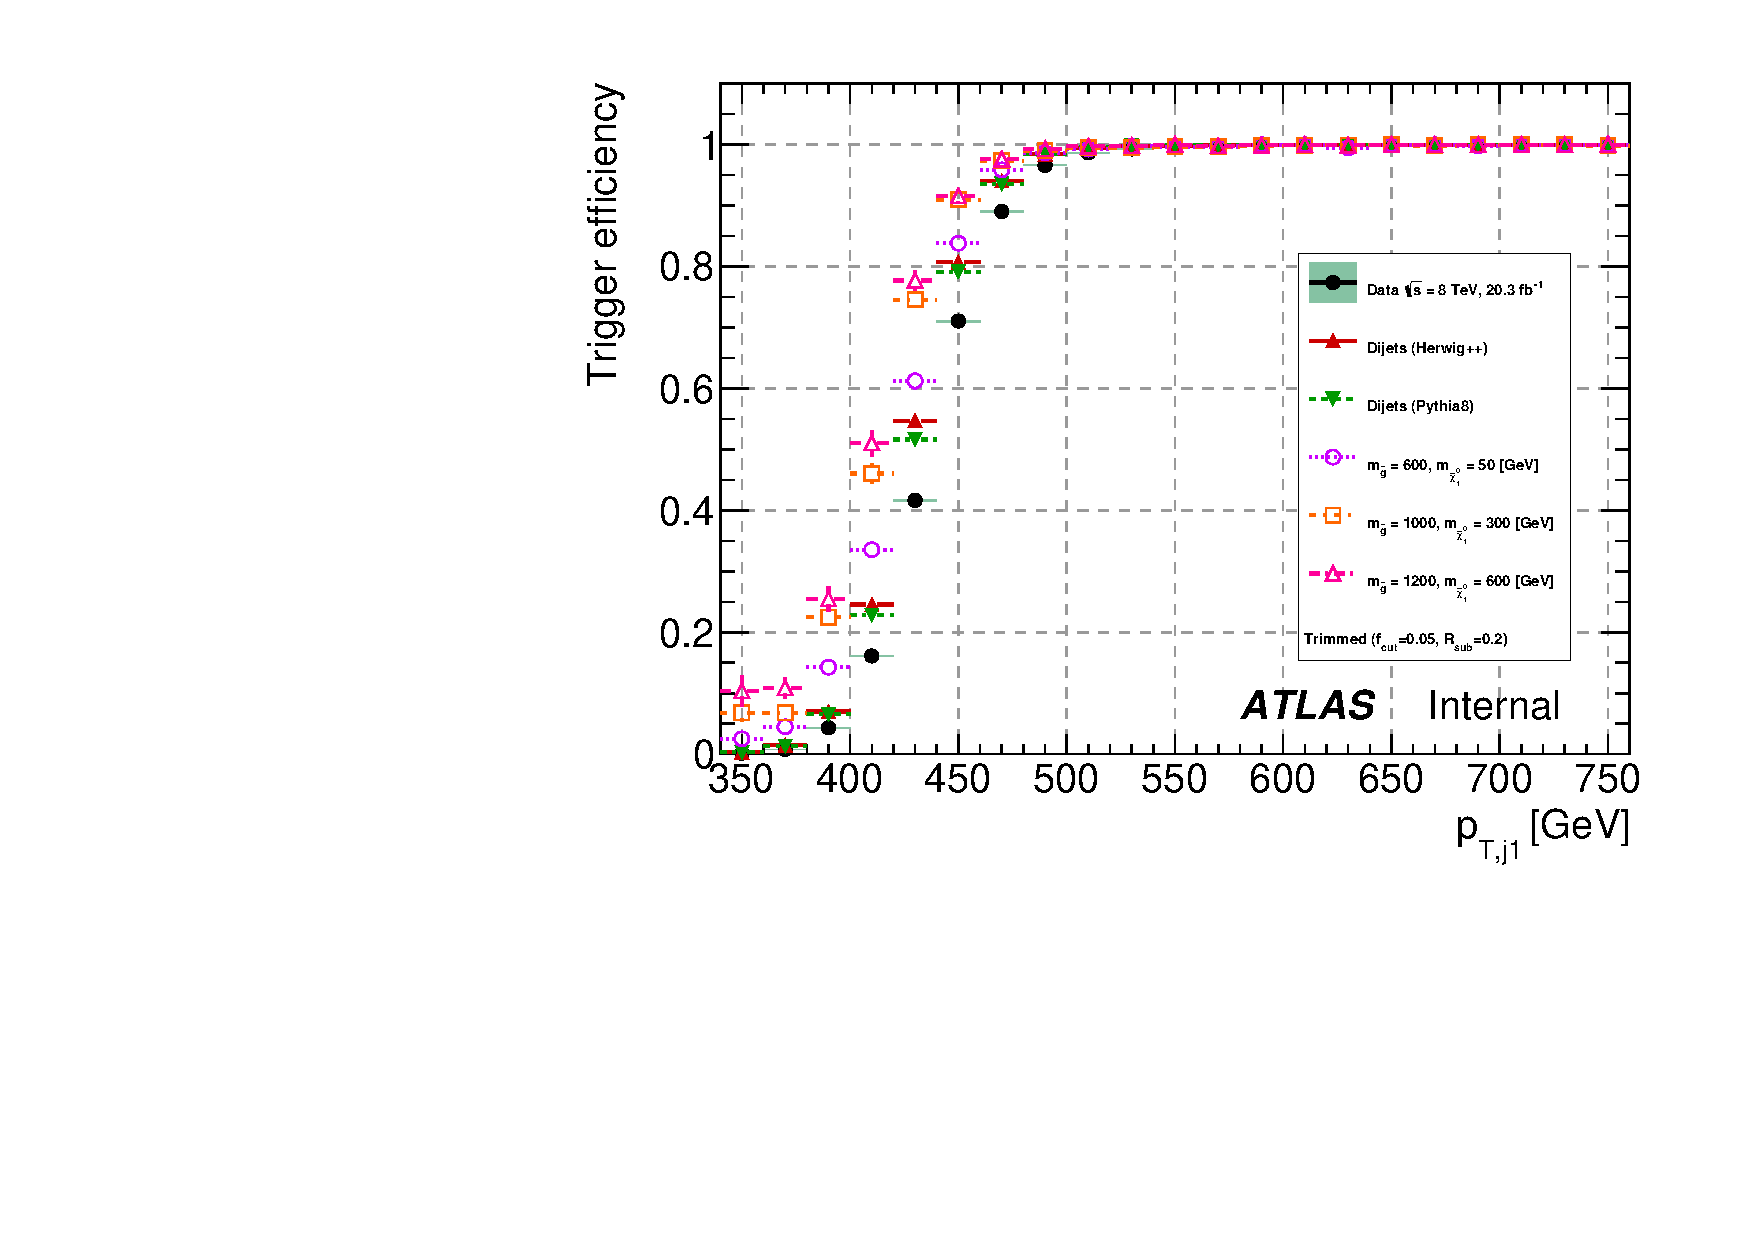
\includegraphics[width=0.48\columnwidth]{INT/Trigger/overlay_Eff_jet_pT1_Trig_10q_Incl_AntiKt10LCTopoTrimmedPtFrac5SmallR30.pdf}
    \label{fig:search:search:trig:pt1:eff}}
  \subfigure[Cumulative efficiency (leading $\ptjet>500$~GeV)]{
    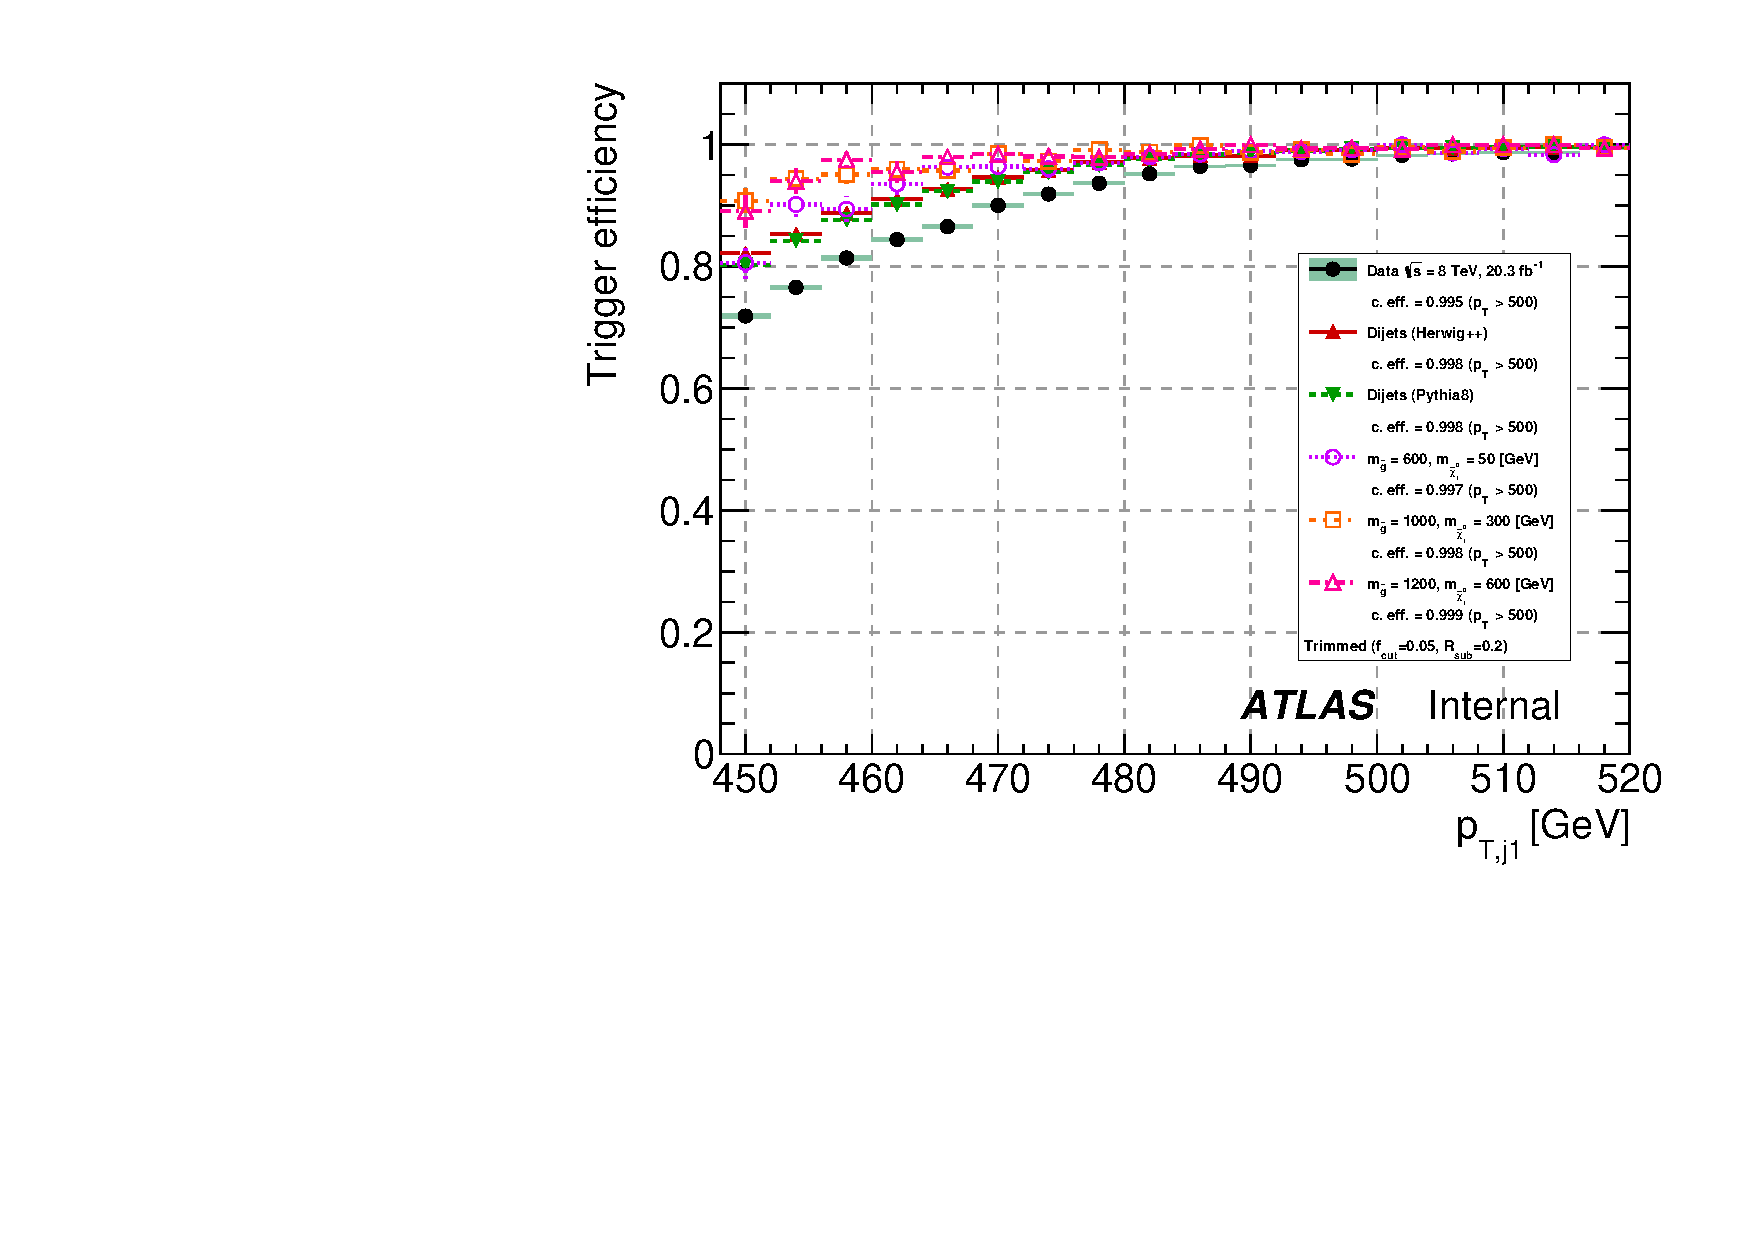
\includegraphics[width=0.48\columnwidth]{INT/Trigger/overlay_Eff_ZoomDetailed_CumEff500_jet_pT1_Trig_10q_Incl_AntiKt10LCTopoTrimmedPtFrac5SmallR30.pdf}
    \label{fig:search:search:trig:pt1:cumeff}}
    \caption{Efficiency for the \texttt{EF\_j360\_a10tcem} trigger as a function of leading $\ptjet$. The efficiency is calculated using \texttt{EF\_j240\_a10tcem} as the reference trigger. The cumulative efficiency (shown in the legend) is the ratio of the sum of the number of events passing the trigger \texttt{EF\_j360\_a10tcem} and the number of events passing the reference trigger \texttt{EF\_j240\_a10tcem}. }
  \label{fig:search:search:trig:pt1}
\end{figure}
%%------------------------------

The \texttt{j360} trigger is fully unprescaled, and the integrated luminosity collected by the trigger (and passing basic detector quality criteria) corresponds to the full 20.3 \ifb ATLAS dataset.

\subsection{Analysis Regions}
\label{chapter:search:search:regions}

Several basic requirements in the analysis have thus been defined: we require high quality events, we use events with several \largeR jets, and we require the leading such jet to have \ptjet > 500 GeV. Two classes of region are now defined: the exclusive 3-jet control region (referred to as the 3jCR) and the various $\geq 4$ jet regions (referred to with the prefix 4j). These are summarized in Figure~\ref{fig:search:search:regions}. 

The 3jCR is inclusive in all variables. This region is strongly enriched in the multi-jet background: a requirement of exactly 3-jets highly reduces the signal in this region (and moreover, the natural cross-section of a 3-jet region is an order of magnitude higher than that of the $\geq 4$ jet region). This makes the 3jCR a perfect candidate for the training sample of the substructure template background estimation technique.

As previously implied in \ref{chapter:search:search:optimization}, $\Deta$'s power is not very strong, but it is rather uncorrelated with \MJ. This means that a selection on $\Deta$ designed to select background-- i.e., a cut on $|\Deta|$ to be high-- can expose a region with high \MJ, but comparatively low expected signal. This allows for the assessment of the templates and the derivation of additional topology related uncertainties, even in the 4j regions. The 4jCR (control region) is defined with $\Deta > 1.4$; the 4jVR (validation region) is defined as $1.4 >\Deta > 1.0$. The two separate regions allow for the derivation of corrections and uncertainties in one, and then the assessment of these in an orthogonal region.

%%------------------------------
\begin{figure}[!ht]
  \centering
  \subfigure[3jCR]{
    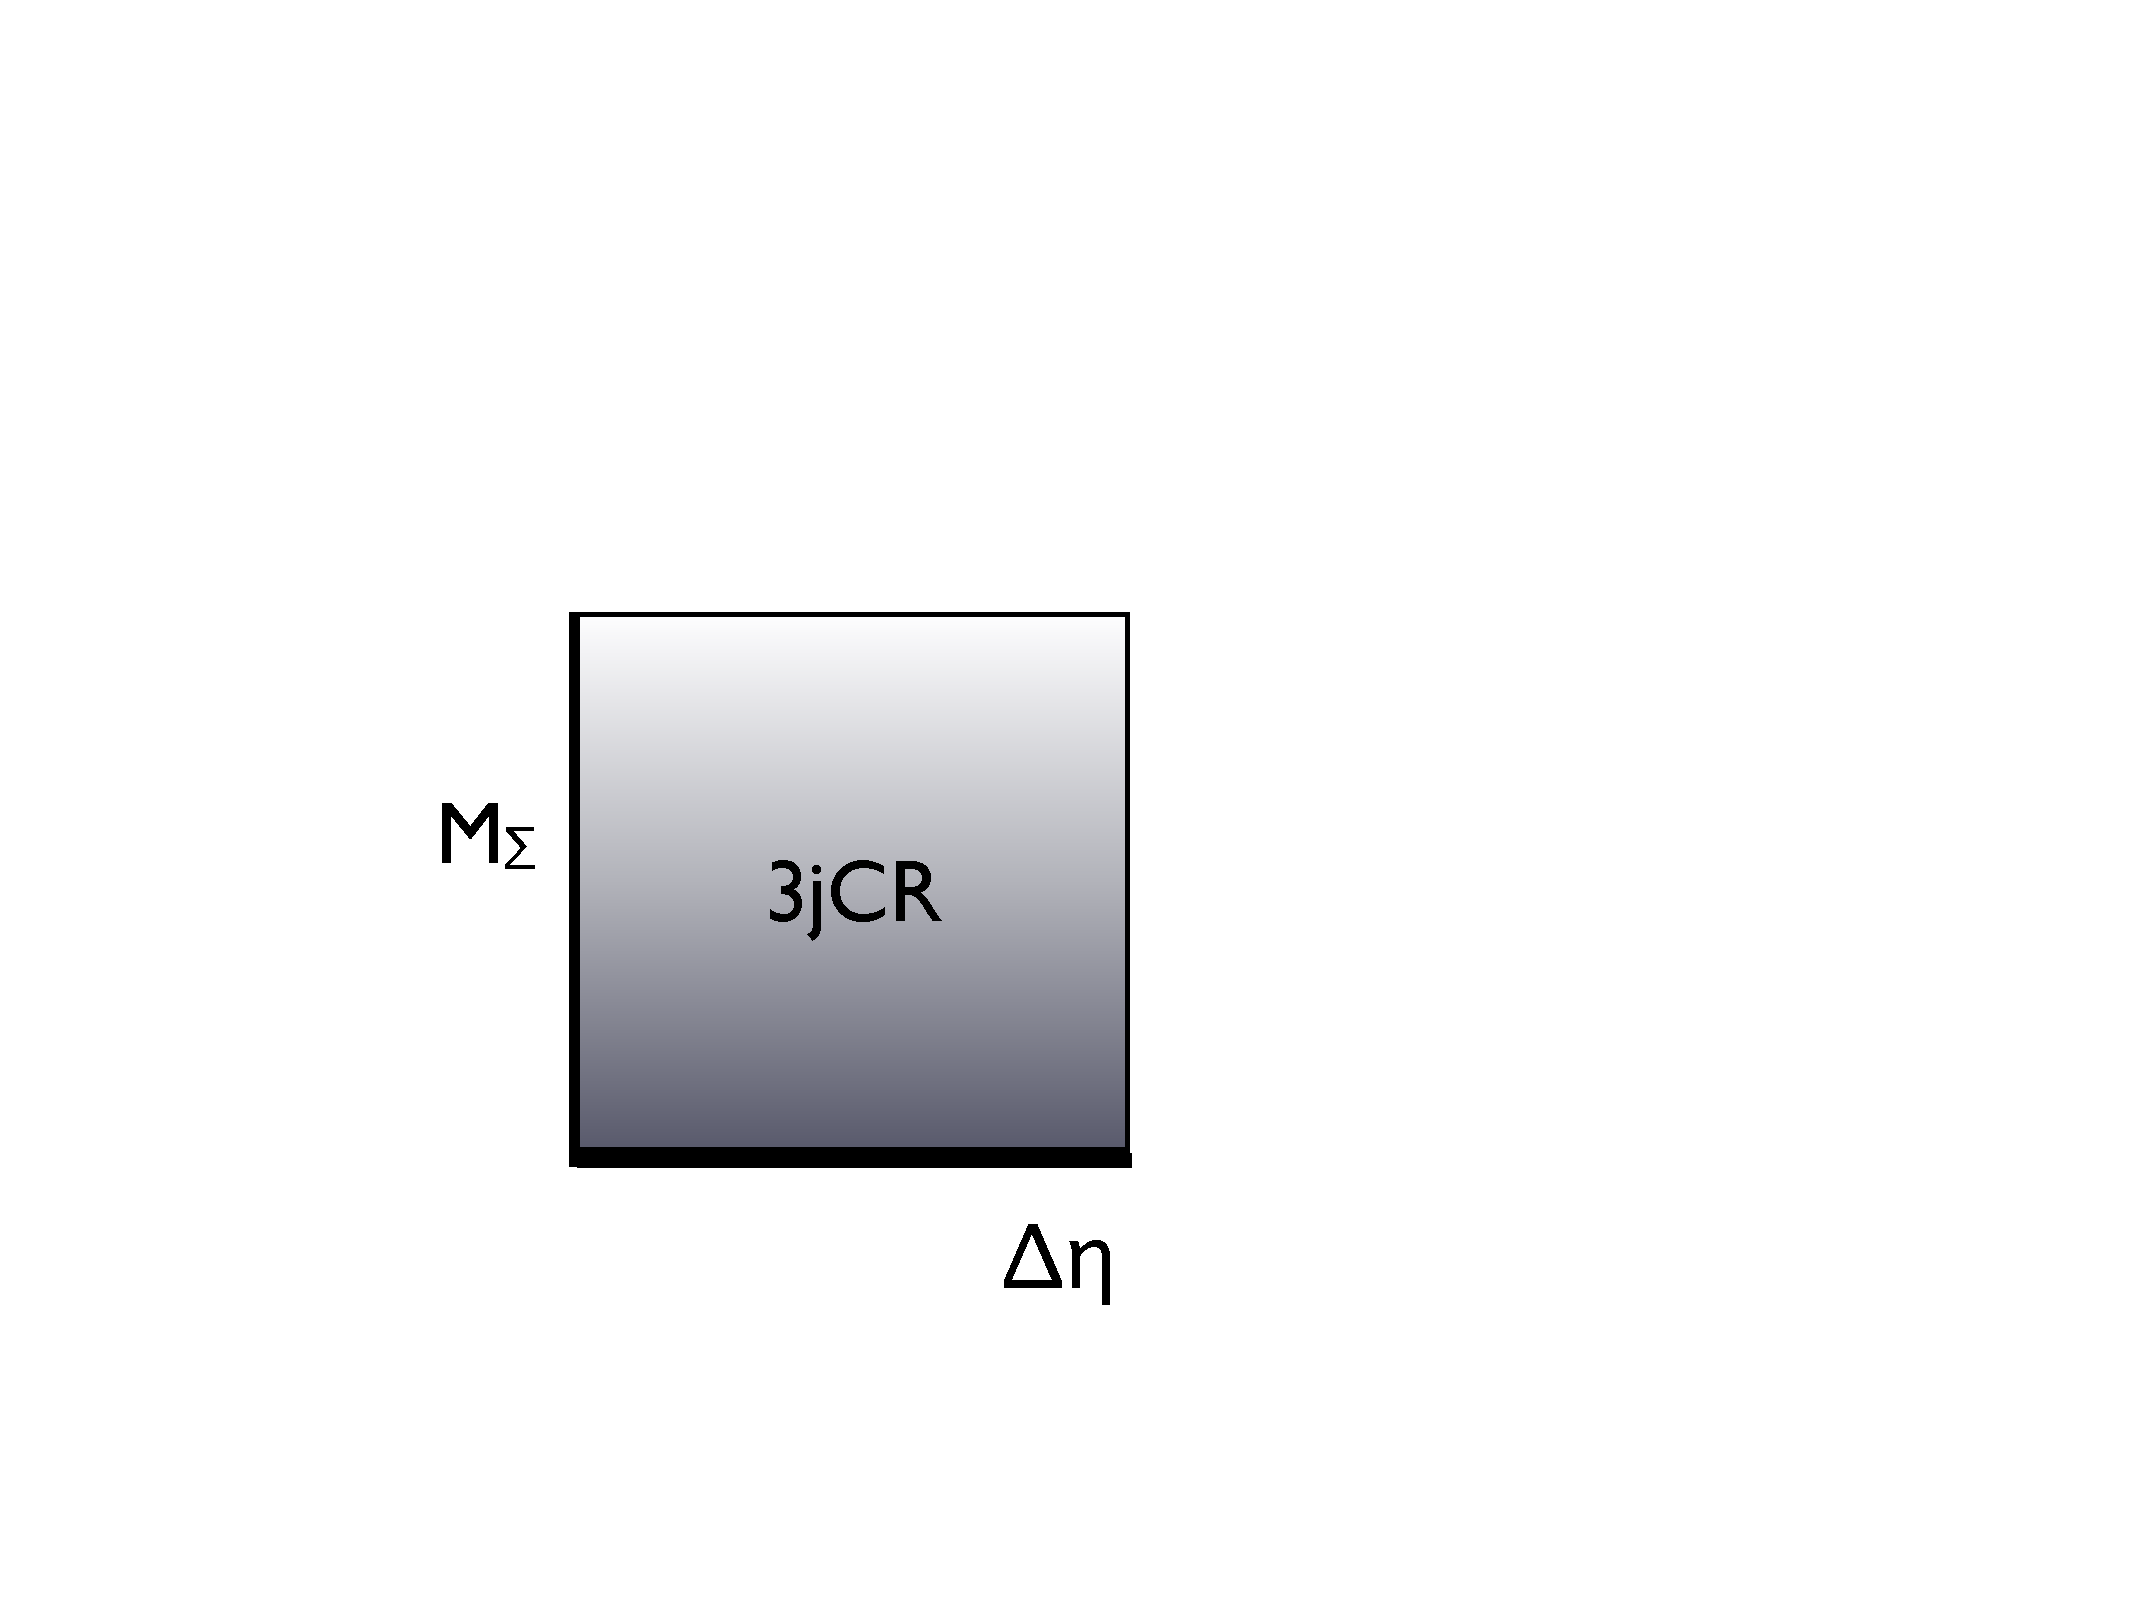
\includegraphics[width=0.48\columnwidth]{INT/3jetsketch}
    \label{fig:search:search:regions:3j}}
  \subfigure[4j regions]{
    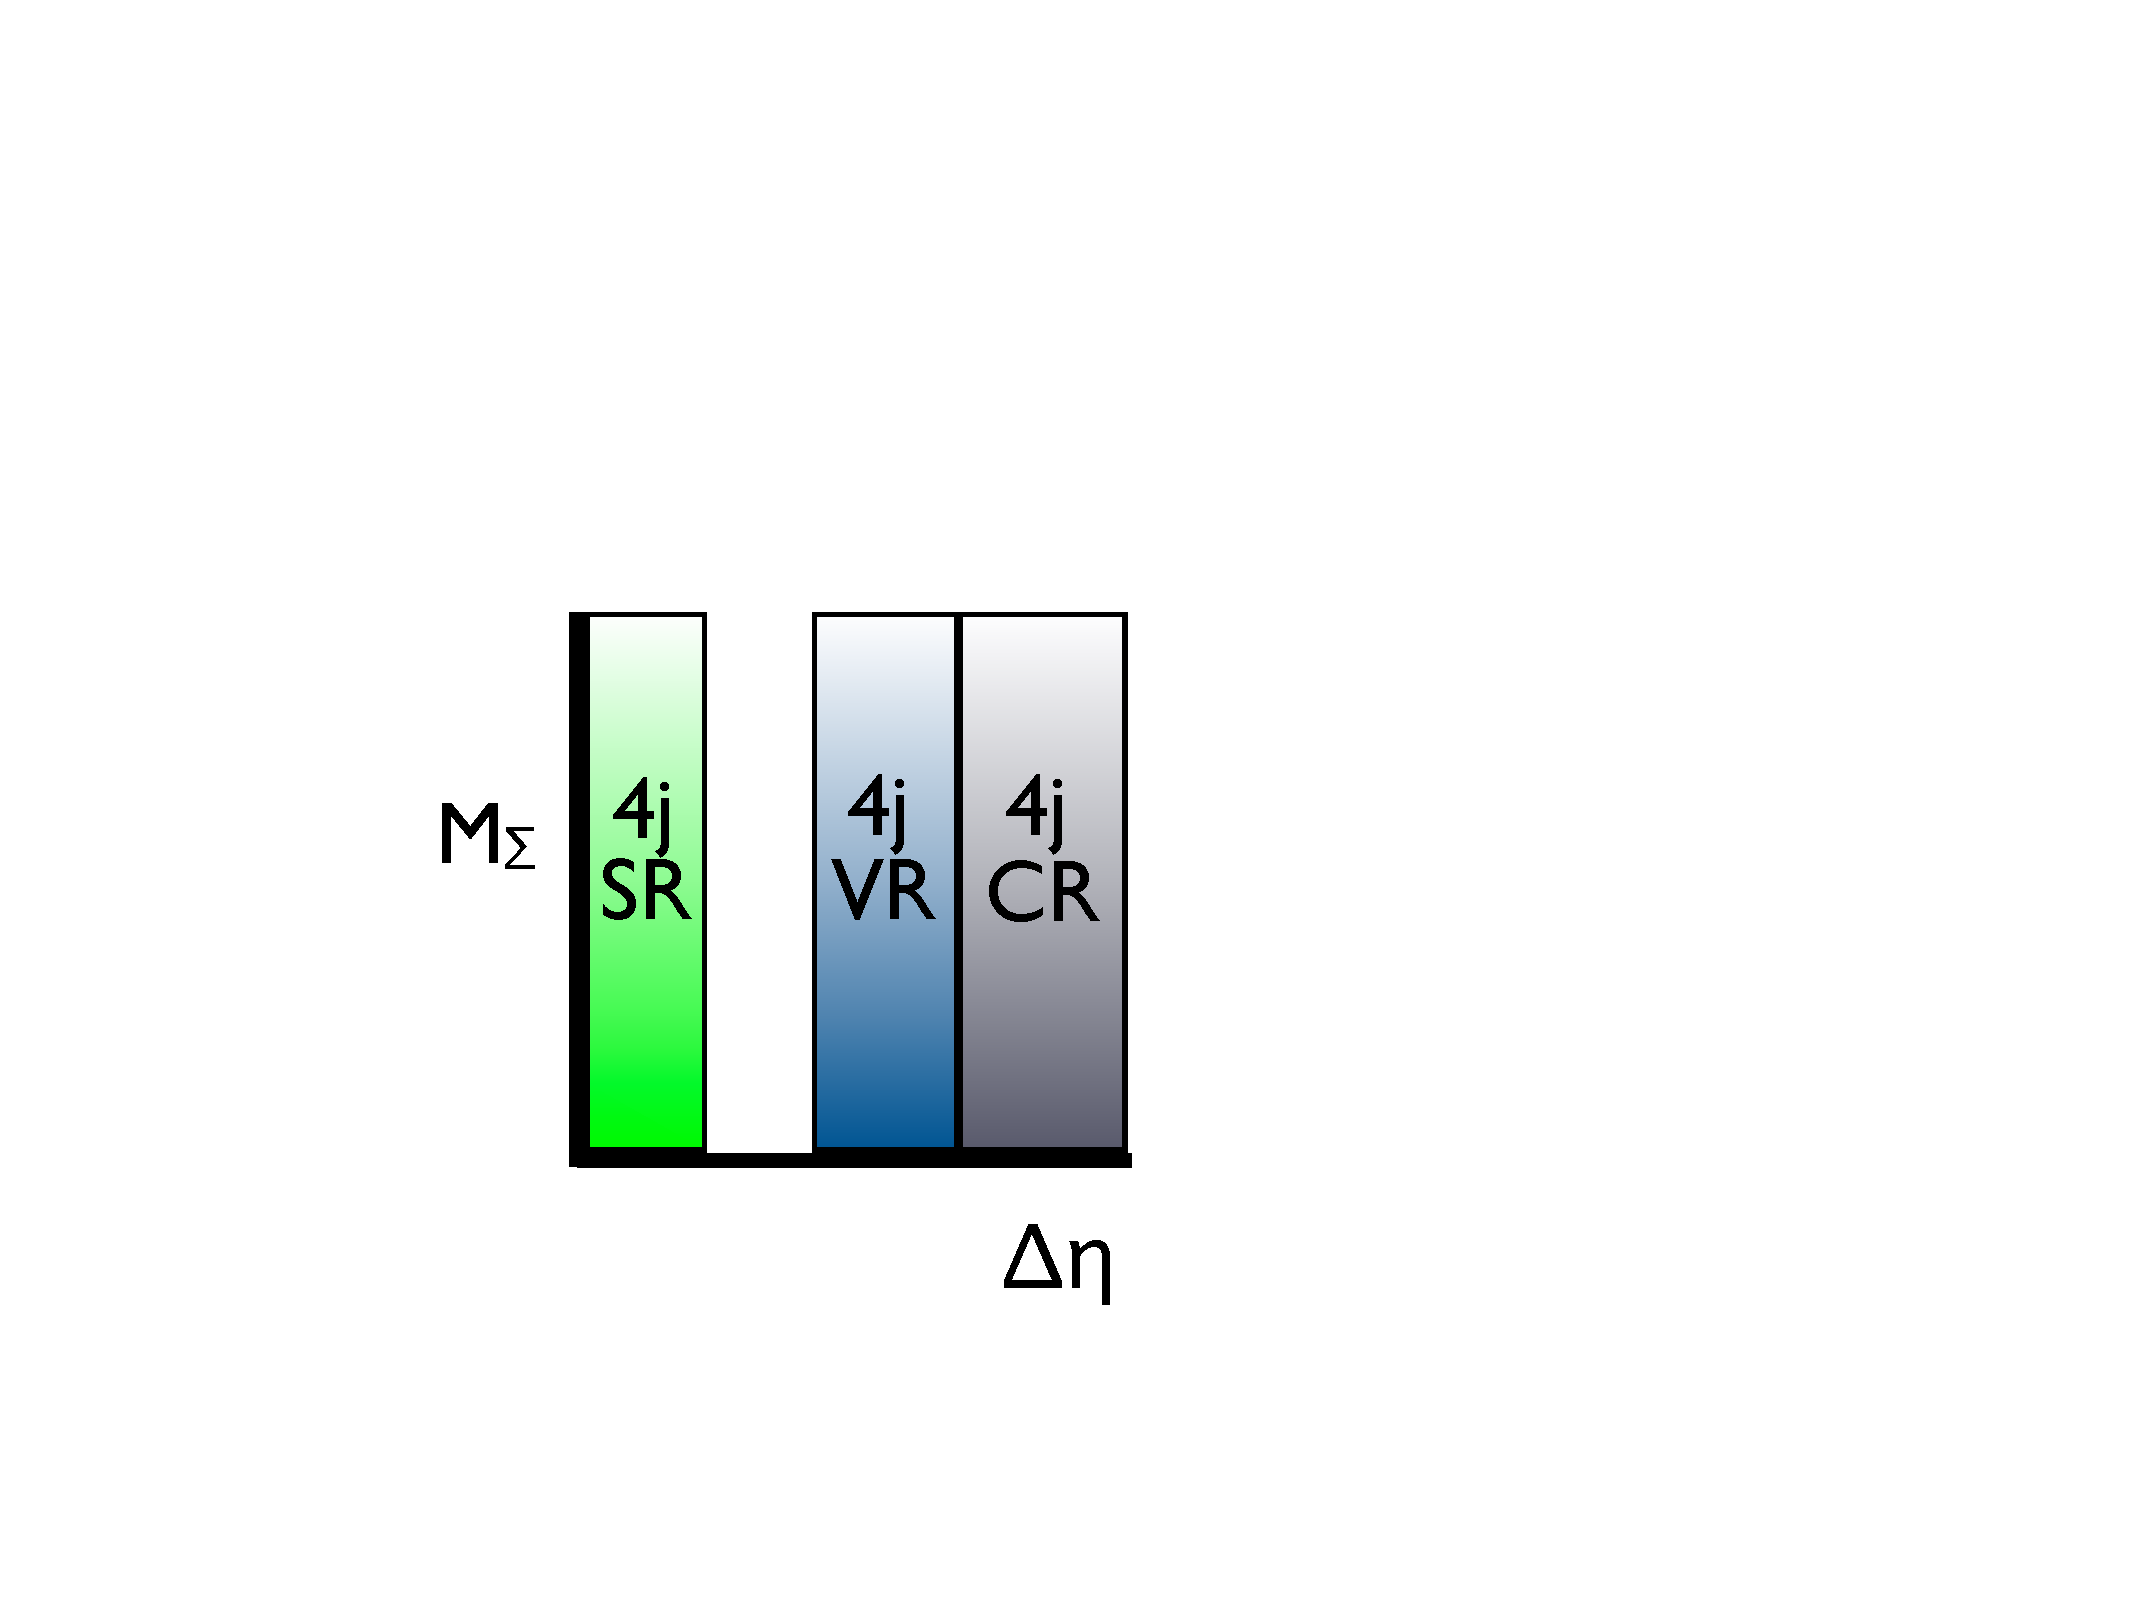
\includegraphics[width=0.48\columnwidth]{INT/4jetsketch.pdf}
    \label{fig:search:search:regions:4j}}
    \caption{Diagrams summarizing the 3j and 4j regions used in the analysis}
  \label{fig:search:search:regions}
\end{figure}
%%------------------------------

One additional set

	
	\subsection{Background Estimates}
	\label{chapter:search:search:background}
	\subsection{Limits}
	\subsection{Future Prospects}
		...